% T10 of the Transport Papers series (consolidated).
% Correction (2026-09-10, mechanical pass, per Leon): rule 23 misidentified T5 as the printed-version exception. T1 is the exception at Version 3.0; every other paper, T5 included, reads Version 1.0. \date corrected accordingly (was 1.1).
% v1.1 (2026-09-10, derivation session, Fable 5.1 subagent, per rule 20,
%   series-review repair pass against series_review_2026-09-09.md).
%   thm:wallfree Level sentence and Sec. Machine verification Part B: the
%     script coverage stated exactly: torsion-level counts, rank 12, symbols
%     and the single surviving component for all three types of dying
%     direction; the K (+) M split and the sigma_2' identity for the
%     Lorentzian and Riemannian types (Riemannian: cosmological term with the
%     opposite sign, sigma_2'(K) - sigma_2'(M) - 2 Lambda = 0); at the null
%     type the wall metric is degenerate and the free sector does not split.
%   thm:action(iii) given its level tag (proved, Stelle-West contraction of
%     Fact mm imported); levels list, assembly clause reworded to name the
%     Goldstone gauge-fixed functional, with (iii) recorded as proved.
%   rem:promotion: "restated accordingly" removed (timeless wording).
%   Part A wording: "a boost" for the SO(2,4) element, matching prop:goldstone.
%   Part C wording: the rho-slot check described as derived from eq:conn.
%   Part B wording: the quoted h_{i,1}, h_{i,2} coefficients now asserted.
%   Printed version 1.0 -> 1.1.
%   Script: verify_T10.py 90/90. Torsion-level checks (rank 18, 3 vacated,
%     rank 16, injectivity on 15, 3 conditions on 9) loop over the three
%     normal forms, the null form in the frame adapted to its dying direction
%     (rows and columns transformed by the null rotation Q); K/M symmetric
%     split, 6 + 6, sigma_2'(M) - sigma_2'(K) with no cross term loop over the
%     Lorentzian and Riemannian forms with D the dying index; the cosmological
%     coefficient checked at all three (-6, +6, and E_0 = +6 = -E_1 at the
%     null form); the rho-slot check now forms nabla_a I_g from eq:conn on a
%     Schouten tensor with rational-function entries in s (no hand derivative);
%     h_{i,2} = (-33/20, -3/40, -3/40) asserted in the Bianchi-series check;
%     docstring version -> printed version 1.1.
%   Compile: pdflatex x2, 36 pages, 0 errors, 0 undefined refs, 0 multiply defined, 0 overfull, no float overflow.
%   Addendum 2026-09-09 (coordinator, same review-repair session): the ButlerT7
%   bibitem subtitle brought up to T7's current title ("State, Continuum, Lift,
%   and the Finite-Ledger Seam"). Bibliography only; nothing else changed.
% 2026-09-09 addendum (interactive session with Leon, Opus 5). Two changes
%   per Leon: (1) the printed version is now 1.0 for every paper T0 to T17,
%   T5 alone at 3.0 (progress-doc rule 23); the development numbering is
%   retired from the title page and kept in this header. (2) Every reference
%   to the programme monograph is removed (rule 24), re-pointed to the series
%   where a sibling paper carries the result and otherwise restated to stand
%   alone. No mathematics, no labels and no numbering changed, so verify_T10.py
%   stands unchanged at 90/90 and was not re-run.
%   Here: the three assembly-level imports of Fact mm are declared by this
%   paper; the ninth refutation now cites the capstone's refutation table.
% v1.13 (2026-09-08, derivation session, Fable 5.1 subagent, per rule 20,
% review-repair pass against T10_review_v8.md; no blocking findings; all S
% items; also N2, N3, N4, N6, N9, N14 in part, N17, and the overfull box):
%   S1 script: family (sI, V/s, s^2 Lambda) built as RF vectors in formal s,
%     differentiated componentwise, evaluated at s = 1, compared with 2 Lambda x
%     the mode; constraints on the family as identities in s; by-construction
%     conjunct dropped (a sign mutation of the mode now fails). S2 script: the
%     two-instance check evaluates the RF Nsq itself. S3 rem:promotion and
%     successor (5): "a known class of modifications (HT; Brown-Teitelboim;
%     Kaloper-Padilla), of which HT is the one used here"; two bibitems added.
%   S4 "not (K)" is Fact 5.10 (fact:notkinematic, provenance T12 Prop 7.6(1)),
%     appended after Rem 5.9; levels list and Position paragraph (eight papers,
%     T12 included, no circularity) updated. S5 the Fact and Prop 5.8(ii)'s
%     proof carry "conformal class unchanged" and say what (K) is. S6 opening
%     of Section 5.1: T12 Prop 7.6 has four clauses, clause (3) has three
%     conditions, the rigidity import is T12 Fact 2.10 citing Prop 5.4 and
%     Prop 4.2(i). S7 fact:weightedlimit restated to T6 Thm 5.11 (all
%     admissible metrics, Def 5.5, fixed Hubble-normalised length) and Cor
%     5.12 (phi-lines, tau^{1/3}); fixed-coordinate-length disclaimer kept;
%     three locators added. S8 Part E paragraph in Section 8. S9 rem:dichotomy
%     sends the items to T11, T12, not sec:verdict. S10 loose-end "residue" ->
%     "open item" (5 sites); pole sense kept. N4: HT is Fact 5.11 (fact:ht).
%   Compile: pdflatex x2, 36pp, 0 errors, 0 undefined, 0 multiply-defined,
%     0 overfull, no float overflow. verify_T10.py 90/90 (unchanged: two checks
%     rebuilt, none added or removed). Numbering frozen: aux diff shows only
%     added labels: fact:notkinematic 5.10, fact:ht 5.11.
%   Knock-on: T6 Def 5.5 should state sum p_i^2 = 1 (Thm 5.11's proof uses
%     it); Fact 4.7 here now says the class requires it.
% v1.12 (2026-09-08, prose pass, Fable 5.1 subagent, per project rule 22: mannered
% prose replaced by literal statement, Leon's ruling to replace the recurring
% vocabulary too; body only, header and script untouched):
%   Compile: pdflatex x2, 35pp (34 before, prose length only), 0 errors, 0 undefined
%     refs, 0 multiply-defined. verify_T10.py 90/90 unchanged. Numbering unchanged
%     (aux diff empty). About 110 replacements.
%   Glossary: ledger -> boundary modes / mode space / boundary-mode bilinear (10);
%     ledger-sphere -> sphere theorem (5); ledger of levels -> levels of the
%     results; verdict -> conclusion (14; labels kept); owned/owns/custody -> shared
%     with / belongs to (4); owed -> still to be supplied; honest dropped; touchpoint
%     -> point of contact (2); joint(s), assembly sense -> step(s) (16; "joint
%     state/flow/action" kept); wing -> summand (4); weld -> matching (4); buys ->
%     yields (3); business -> task (2); kills -> removes/makes vanish; hard to kill ->
%     hard to refute; seam -> the ell_P^2/A corrections; frontier -> open problem;
%     pinned -> fixed; sits -> is; lives in -> lies in; debts -> prior work;
%     standing in -> working substitute; skeleton -> content.
%   Non-glossary: does not shake -> has no physical fluctuation (prop:goldstone);
%     grip (verb) -> couple, selective grip -> selective coupling (result names
%     kept); null ruler -> null vector; needs no ruler -> action needs no metric;
%     as mortal as -> degenerate exactly where (thm:twokinds); scar dropped; escape
%     -> way to avoid refutation; takes no comfort in -> does not rely on; trap ->
%     error to avoid; habitat -> setting; door -> residue; ceiling -> bound; price
%     -> consequence; story -> behaviour; banked -> recorded; blocked behind ->
%     cannot be addressed until; hinge -> depends on; touch -> change; sound in a
%     gas of correlations -> an acoustic mode of the correlations.
% v1.11 (2026-09-07, derivation session, Fable 5; gap-analysis fold-in of the
% four-programmes note's Section 4, per gap_merge_plan_2026-09-07.md):
%   Compile: 34pp, 0 errors, 0 warnings, 0 undefined refs, 0 multiply-defined,
%     0 overfull; verify_T10.py 90/90 (83 prior + 7 new, Part E). Frozen
%     numbering (rule 21) preserved: aux diff against v1.10 shows every
%     pre-existing label at its old number; the new material is a
%     subsection at the end of Section 5, after Asm 5.5.
%   (1) New Section 5.1 (subsec:fourth): Def 5.6 (four ways a conserved
%     number enters a theory: kinematic, dynamically fixed, parameter of the
%     laws, initial data); Prop 5.7 (the four are exhaustive and disjoint on
%     D/P/I, the three are not, so "not kinematic, not dynamical, therefore
%     initial data" needs (P) excluded); Prop 5.8 (under the action as
%     written N = M_P/H is a parameter of the laws: Lambda indexes the
%     theory, the norm cannot fluctuate by Prop 5.4's count, d(N^2)/dLambda
%     = -3 M_P^2/Lambda^2; with Lambda free the count is 13 - 3 = 10 against
%     a 9-dimensional gauge orbit, one norm mode (I/2Lambda, -V/2Lambda, 1),
%     the tangent of the rescaling family, with no equation of motion);
%     Rem 5.9 (the Henneaux-Teitelboim promotion reconciles (P) with T12's
%     initial-data reading and is a decision for the series, not a theorem;
%     left open, both branches stated: adopt and recompute the Goldstone
%     count with the norm mode and its conjugate time, or reject and
%     withdraw the dating observation from initial-data status).
%   (2) Contribution (3), the ledger's Proved and Readings paragraphs, the
%     Position paragraph on T12, and successor (5) (now "the smallness of
%     Lambda, and the promotion decision") updated; Section 8 says five
%     parts and ninety checks.
%   (3) Bibliography: HenneauxTeitelboim1989 added.
%   (4) script: Part E appended before the summary: d(N^2)/dLambda as an RF
%     identity; N^2 unequal at Lambda = 3, 12; free-Lambda rank 3 on 13;
%     gauge images rank 9 with a zero dLambda column; the norm mode
%     satisfies the free constraints and violates the fixed; images plus
%     the mode rank 10; the mode equals 1/(2 Lambda) times the s-derivative
%     of (sI, V/s, s^2 Lambda) at s = 1, the family constrained for three
%     rational s. Note: the script's cons_T rows omit the factors 2, so the
%     dLambda columns are -1/6 and -3/(2 Lambda^2). All 7 substantive.
%   Knock-on recorded, not applied: T12 prop:trichotomy gains the fourth
%     alternative and clause (3) rests on the promotion (T12 v1.6); T17
%     Table 4 row 8.
%   Not done here (rule 20): milestone ticks, Run log, tp_status, sync.
% v1.10 (2026-09-02, derivation session, Fable 5; T10_review_v6.md CLEARED the
% paper at v1.9 with a tidy list; this version applies items 1-9 of that list,
% none of which changes a conclusion):
%   1 duplicated clause in prop:w(ii) removed; 2 "vanishing interior
%   variation" at the three remaining sites (thm:action(2) proof, ledger,
%   "not checked" list); 3 "and tangential legs" deleted from Section 8;
%   4 counterterm proof names the terms with their prefactors 2 and Lambda/3
%   and their densities separately; 5 the dangling gloss in Section 8
%   re-attached to the I-perp facts; 6 inventory: rho-slot check listed in
%   Part C, the Lambda = 3 instance in Part A, the unit-boost check attributed
%   to kasnerwall(ii); 7 the prop:w checks now apply eq:conn to I_g with a
%   symbolic Schouten tensor (all three slots; the rho slot's algebraic part
%   computed, its derivative part (1/4) d_a J checked), Section 8 wording
%   matches; 8 the unit-boost check tests two independent vectors of the
%   complement; 9 asm:forcing's closing sentence cites joint 1.
%   Item 10 (the abstract's six-clause shape) is a decision for Leon and is
%   left as it stands; item 11 (downstream drift in T11, T14, T17) is the
%   standing knock-on for the mechanical pass, now to be scheduled.
%   Numbering unchanged. verify_T10.py: 83/83 (two prop:w checks rebuilt, one
%   removed as subsumed, one added). Compile: pdflatex x2, 0 errors,
%   0 undefined references, 0 em dashes.
% v1.9 (2026-09-02, derivation session, Fable 5; addresses T10_review_v5.md,
% the re-review of v1.8: all four new blocking findings and the non-blocking
% list):
%   NEW 1 thm:action(iii): the field space is the metric connections with
%   nabla I = 0 (those reducing to I-perp), which IS fact:mm's; carried to
%   itself by the gauge group since (g nabla g^-1)(gI) = g(nabla I); the
%   twenty extra components of an unconstrained connection are nabla I and
%   enter the Lorentz block quadratically via [I^u, I^v] = -<I,I> u^v
%   (script-checked, with eps(I,V,u^v,B) != 0). I declared a field with
%   <I,I> = Lambda/3 (NB 1).
%   NEW 2 verify_T10.py: the generic transgression connection now has legs
%   in all four directions (range(4)); docstring and check string corrected;
%   Section 8 says "legs in all four coordinate directions".
%   NEW 3 abstract: "at the Schwarzschild wall".
%   NEW 4 thm:action(1) cites kasnerwall "on the Kasner model, transported by
%   fact:weightedlimit"; the carve-out says "the Schwarzschild exponents
%   included"; kasnerwall's Level line routes Schwarzschild and SdS through
%   the Fact.
%   Non-blocking: AdS branch script-checked at Lambda = -3 (I-perp (2,3));
%   {I,V}-perp (1,3) checked on both branches; prop:w given a proof block
%   (the slot computation moved there) and the rho slot (1/4) d_a J checked on
%   a non-constant-J instance; "vanishing interior variation" at both sites;
%   Section 8 inventory (two lambdacorr parameter sets, the unit-boost
%   check, which now forms B_w^2 exactly rather than re-checking sum p^2);
%   check 58's string reduced to what it computes; "the statements of (i) and
%   (ii)" in the carve-out; normalising factors |<I,I>|^{1/2}, |<V,V>|^{1/2}
%   with product 1 on both branches; the (1,3) subtraction written for both
%   branches; whichwall(iv) in the (nabla, I, V) form; "not checked" list adds
%   the Einstein identity -4 Ric^2 + R^2 = 0 and the unused Fock clause.
%   KNOCK-ON for the mechanical pass / Leon: downstream drift in T11, T14,
%   T17 as flagged since v1.6, sharpened in T10_review_v5.md item 15.
%   Numbering unchanged. verify_T10.py: 83/83 (was 79: +AdS signature,
%   +{I,V}-perp signature, +field-space certificate, +rho slot).
%   Compile: pdflatex x2, 0 errors, 0 undefined references, 0 em dashes.
% v1.8 (2026-09-02, derivation session, Fable 5; addresses T10_review_v4.md,
% the re-review of v1.7: all seven new blocking findings and the non-blocking
% list; every item bookkeeping, no conclusion changed):
%   NEW 1 prop:w(ii): the rho slot of nabla I_g is (1/4) d_a J, not zero; the
%   clause now argues mu-slot iff Einstein, Einstein => R constant (contracted
%   Bianchi) => rho slot vanishes with it.
%   NEW 2 ledger: goldstone's invariance moved to "Proved"; the assembly
%   paragraph keeps only the identification with the MM functional.
%   NEW 3 prop:kasnerwall carve-out widened: (i), (ii) displays and the GB
%   density hold verbatim for the exact Kasner metric at Lambda = 0,
%   Schwarzschild included; Lambda != 0 needed only for the action's form.
%   NEW 4 thm:action(1) says "At the Schwarzschild wall"; ledger attributes
%   the SdS transport to fact:weightedlimit.
%   NEW 5 kasnerwall's Level line: sphere rates tau^{1/3} rotations,
%   tau^{2/3} boosts.
%   NEW 6 thm:action(i),(ii) carry both branches (SO(1,4)/(1,4) for
%   Lambda > 0, SO(2,3)/(2,3) for Lambda < 0), with {I,V}-perp (1,3) on both.
%   NEW 7 thm:action(iii) states the field space of nabla: the metric
%   connections of the ambient bundle (fact:mm's), eq:conn being the point at
%   which the canonical solution sits; generic gauge transformations do not
%   preserve the tractor shape, hence the whole space.
%   Non-blocking: ~ on both display lines; consequence (1)'s proof argues on
%   eps(I,V,F,F); "5 + 4" replaced by the fibration description; Kretschmann
%   named for the tau^{-4} rate; "second of the two answers"; verification
%   inventory lists the SO(2,4) invariance and the Milne point;
%   fact:weightedlimit states the SdS case (T6 Thm 5.9); "not checked" list
%   adds the GB variation and the C criterion; prop:nogo gets a Level line
%   and its (Q)-state derivation moved from statement to proof; psi_k named;
%   I_g reconnected to I; script docstring 1.7 -> current, boost comment
%   corrected, covariance check string in array symbols; dQ = eps R^R now
%   also checked on a generic connection with all six components (the quartic
%   step exercised).
%   KNOCK-ON for the mechanical pass / Leon: downstream drift in T11, T14,
%   T17 as flagged since v1.6.
%   Numbering unchanged. verify_T10.py: 79/79 (was 78). Compile: pdflatex x2,
%   0 errors, 0 undefined references, 0 em dashes.
% v1.7 (2026-09-02, derivation session, Fable 5; addresses T10_review_v3.md,
% the re-review of v1.6: all eight new blocking findings and the non-blocking
% list):
%   NEW A: thm:action(iii) now displays S[nabla, I, V] on one line and its
%   value at the canonical solution V = X - (3/Lambda) I on a second;
%   consequence (1) and thm:twokinds(2) say "I and V"; the contribution
%   list, the figure label and the caption advertise the nine-to-nine count
%   (the rank-5 check is fact:frozen's).
%   NEW B: prop:kasnerwall(ii)'s Ricci displays negated to T6's convention
%   (de Sitter Ric = +Lambda g, P = +(Lambda/6) g): tau^2 R_00 = S2 - S1,
%   tau^2 R_ii = -p_i (S1 - 1); the contraction Ric_{bd} = -R^a_{bad} stated
%   in the proof with the reason; the script's Ricci routine carries the
%   same sign and comment, and the non-Kasner check certifies the corrected
%   displays.
%   NEW C: hypothesis p1 p2 p3 != 0 added (excludes the Milne point (1,0,0));
%   "no chart" argued from the Euler density = sqrt|g| Kretschmann on an
%   Einstein metric (-4 Ric^2 + R^2 = 0); script runs (1,0,0) and confirms
%   every coefficient vanishes there.
%   NEW D: prop:lambdacorr's proof no longer places SdS in the Bianchi I
%   class; T6 Thm 5.9 cited for what it gives (shared residue and rates).
%   NEW E: ledger line for whichwall(iv) says "open" as the body does, with
%   the Bianchi I / SdS computation attributed correctly.
%   NEW F: C implemented at mode level (C psi_k C^-1 = psi^dag_{-k}); the
%   criterion n_{-k} = 1 - n_k proved from the two-point function; the
%   window/array dictionary stated in Part D and in the script.
%   NEW G: the diagonal charged check labelled an identity; the superposition
%   check carries the content; Part D prose claims necessity only.
%   NEW H: even-power system corrected to (2n+1) c_i + p_i sum c_j = 0,
%   n >= 0, with the three terms named.
%   Non-blocking: (b)'s proof notes de enters as a source; abstract and prior
%   art scoped "on the flat model ... exactly one scalar relation"; ledger
%   thm:wallfree line scoped; counterterm assumes Lambda != 0; sphere rate
%   tau^{1/3} in lambdacorr's statement; calP consistent; abstract 248 words;
%   withdrawn-claim count reworded (one withdrawn claim, two negative
%   controls); ledger flags fact:weightedlimit values-level and fact:cft's
%   Sugawara use; fact:walls drops the Thm 8.27 locator; front matter carries
%   the Indifference and (Q) conditions; T6's transport-level statement quoted
%   correctly (withheld along the phi lines only); "not checked" list
%   extended; prop:goldstone's covariance PROVED (SO-invariance of the
%   contraction) and script-checked on rational SO(2,4) elements, its Level
%   line upgraded, the invariance argument spelled out (gauge action on
%   nabla, F, I, V; isometry preserves the prefactor and constraints;
%   pointwise identity integrates); fact:mm states the AdS branch.
%   KNOCK-ON for the mechanical pass / Leon: T14:113 and T17:217 describe the
%   no-go as the I-sector closed at every door; now the (I,V)-sector with the
%   (Q) and Indifference conditions; T17's and T11's stale T10 rows as before.
%   Numbering unchanged. verify_T10.py: 78/78 (was 76: +(1,0,0) point,
%   +SO(2,4) invariance). Compile: pdflatex x2, 0 errors, 0 undefined
%   references, 0 em dashes.
% v1.6 (2026-09-02, derivation session, Fable 5; addresses T10_review_v2.md,
% the three-agent review of v1.5, all eleven blocking findings and the
% mechanical list):
%   BLOCK 1 prop:goldstone: rebuilt on the three-argument functional
%   S[nabla, I, V] with V an independent constrained field (the reviewer's
%   counterexample xi = I^V, acting on nabla and I with X fixed, changes the
%   integrand by minus itself, now recorded in the proof); constrained
%   fluctuation space 5 + 4 = 9, stabiliser of (I,V) = so(1,3) dim 6, broken
%   15 - 6 = 9, bijective: exact eating. The four-dimensional sentence removed
%   (that is asm:lift's). thm:action(iii) says the functional is written in
%   the scale I determines and that V is a constrained field in the
%   variational principle; the prefactor chain restated via <I,I><V,V> = -1
%   (both signs of Lambda). Script: rank 9, constraint independence, the
%   one-argument failure (4 checks).
%   BLOCK 2 thm:wallfree: concluding sentence, abstract and introduction
%   scoped to the flat model of (d); on a curved wall only (c) survives; the
%   curved-wall jet count posed as successor 2.
%   BLOCK 3 prop:kasnerwall: re-posed on the Bianchi I Einstein-Lambda family
%   of prop:lambdacorr (moved before it, now 4.8; kasnerwall 4.9), with the
%   exact Kasner metric as leading term; Lambda = 0 statements confined to the
%   bare Gauss-Bonnet integrand; "no chart" now argued from the Kretschmann
%   invariant; the schematic Lambda sentence replaced by a pointer.
%   BLOCK 4 lem:varexp: tangential sign corrected (omega^{ij} = log tau
%   [(d_i p_j) tau^{-p_i} e^j - (d_j p_i) tau^{-p_j} e^i], convention
%   omega^i_j = -omega^{ij} stated); script: torsion-free as an exterior-
%   algebra identity with placeholder coefficients, and the opposite sign
%   fails (2 checks).
%   BLOCK 5 T8 Indifference premise (Principle 5.4) attached in fact:walls,
%   asm:lift joint 4 re-headed conditional, ledger lines added.
%   BLOCK 6 fact:current carries T5's premise (Q) (Premise 8.1) for
%   thermality and the assembly flag + Pressley-Segal root for the charge-zero
%   Fock isomorphism; prop:nogo derives the C-invariance of the (Q) state from
%   n_{-k} = 1 - n_k at the sea level and is conditional on (Q) there.
%   BLOCK 7 fact:weightedlimit: rates O(tau^{2/3}) boosts, O(tau^{1/3})
%   rotations, values-level; asm:forcing joint 1 likewise.
%   BLOCK 8 the two tautological Part D checks replaced by the charged-case
%   overlap in the diagonal state (zero) and in a two-sector superposition
%   (nonzero); the "every check could fail" sentence replaced; twokinds checks
%   labelled identities.
%   BLOCK 9 prop:counterterm(iii): "interior" equations; the counterterm is
%   the boost block (extrinsic curvature), not the induced connection; frame
%   dependence of Q stated (defined relative to the exceptional frame).
%   BLOCK 10 prop:lambdacorr closing sentence restricted: regularity in
%   Bianchi I only; at Schwarzschild-de Sitter the Kantowski-Sachs sphere adds
%   O(tau^{2/3}) relative corrections; only the residue statement survives.
%   Constraint propagation (dC/dtau = 2S(Lambda - C)) and odd-powers argument
%   added.
%   BLOCK 11 monograph cited with locators (Thm 12.15, Thm 13.13) wherever
%   "the monograph" is invoked.
%   Mechanical: caption (3)->(2); orbit label U not X; "v1.0"/"earlier drafts"
%   removed from body and script strings; script docstring and prop:vacate
%   tags -> thm:wallfree(a); ledger lines for whichwall(iv) and goldstone's
%   assembly dependency; T1 in the Position section and named at the proof
%   standard; Position split into two paragraphs; fact:cft chapter locators
%   and clause 2 dropped; <k,k*> = 1/2 per T4 with the rescaling noted; Gover
%   attached to fact:frozen; asm:lift joint 3 (invertible region, LDG root);
%   T4 locator 7.3-7.4; grammar at the head of Section 5; prop:w(i) carries
%   the p = -rho line; twokinds(1) "one per simple factor"; the state in
%   prop:nogo renamed varphi, the four-plane calP, the charge Q_c; nogo's
%   "sector" made precise (C-even neutral subalgebra, larger than the T family
%   thermally). PressleySegal1986 bibitem added.
%   KNOCK-ON for the mechanical pass / Leon (review item 5): T17's ledger row
%   for T10 and T11's Fact still describe the v1.0 identification and "action
%   iff Lambda != 0"; page and check counts stale (29pp, 76 checks).
%   Numbering: Prop 4.2, Thm 4.3, Section 5 unchanged; lambdacorr is now 4.8
%   and kasnerwall 4.9 (neither cited elsewhere).
%   verify_T10.py: 76/76 (was 70). Compile: pdflatex x2, 0 errors,
%   0 undefined references, 0 em dashes.
% v1.5 (2026-09-02, derivation session, Fable 5, same day; discharges the
% three qualifications left by v1.4's asm:forcing):
%   prop:lambdacorr (proved): Bianchi I with Lambda has a unique formal
%   solution with residue p at the wall, H_i = p_i/tau + (Lambda/2)(1-p_i) tau
%   + odd higher orders, all coefficients determined by the evolution
%   equations with the constraint then identical (Bianchi): the residue is
%   Lambda-independent, corrections regular; applies to Schwarzschild-de
%   Sitter via T6 Thm 5.9. Script: series solved to tau^5 at the Schwarzschild
%   exponents, Lambda = 3, residuals zero through tau^4.
%   prop:counterterm (proved): the Chern-Simons primitive Q of eps R^R; on a
%   Kasner slice Q = 8 p1 p2 p3 eps^-2 d^3x (script: exact, both Kasner
%   points; dQ = eps R^R confirmed identically); adding (3/Lambda) int_wall Q
%   removes the divergence exactly, leaves the field equations untouched,
%   and leaves an O(Lambda) scheme constant as the only ambiguity; the
%   counterterm coefficient is sigma_3 of the residue.
%   lem:varexp (proved by hand, classical diagonal-metric formula): for
%   tau^{2 p_i(x)} metrics on the open Kasner circle the boost block is the
%   pointwise Kasner pole with no correction and the tangential block is
%   log(tau) tau^{-p_j} (dp): subleading (p_max < 1); all curvature corrections
%   are of relative order tau^{1-p_max} log^2: the leading equations are the
%   pointwise Kasner relations and the counterterm is pointwise. Momentum
%   constraints and the non-diagonal class stated as NOT done (rem:remains).
%   asm:forcing's closing paragraph, successor 1, ledger, introduction and
%   verification section updated. Numbering of Prop 4.2 / Thm 4.3 / Section 5
%   unchanged (new items are 4.10-4.13).
%   verify_T10.py: 70/70 (was 62). Compile: pdflatex x2, 0 errors,
%   0 undefined references, 0 em dashes.
% v1.4 (2026-09-02, derivation session, Fable 5, same day; answers the
% interface question posed in v1.3 for the Schwarzschild wall):
%   Reading T6's weighted-limit theorem (Lems 5.1-5.4, Thm 5.6, Thm 5.9) with
%   T4's weld (Thm 8.16, Prop 8.26, Thm 8.27) gives the answer: at the
%   Schwarzschild singularity the datum's connection has a SIMPLE POLE with
%   tangential legs and residue the Kasner boost. New Section 4.5:
%   fact:weightedlimit (imported); prop:kasnerwall (proved on the Kasner
%   model, exact): (i) in the exceptional (orthonormal) chart I, X, the
%   soldering form and both wings of the tractor connection are regular; the
%   only singular piece is the Levi-Civita block omega^{i0} = (p_i/tau) e^i, a
%   simple pole with residue sum p_i B_i (x) e^i, NOT a gauge pole (curvature
%   is a double pole with tangential legs); so the datum extends regularly in
%   NO chart. (ii) tau^2 R_00 = -(sum p^2 - sum p), tau^2 R_ii = p_i(sum p - 1):
%   the field equations at the wall are the Kasner relations, conditions on
%   the residue; sum p^2 = 1 says the residue bivector is a unit boost.
%   (iii) action densities on the Kasner approach: Gauss-Bonnet
%   -16 p1 p2 p3 tau^-3 (64/27 tau^-3 for Schwarzschild, non-integrable),
%   Einstein-Cartan O(Lambda tau), cosmological 24 tau: the curvature-squared
%   VALUE diverges through the exact topological term alone; the variational
%   principle and equations reach the wall. asm:forcing (assembly, joints
%   itemised): the pole is not removable, its residues are fixed by the
%   equations, and those residues are the completion's weights (T4 Thm 8.16):
%   the forcing half is answered in the residue sense for the constant-
%   exponent class: the equations neither permit nor demand the completion,
%   their singularity supplies its data. thm:action(1) qualified accordingly
%   (equations, not the number); prop:whichwall(iv) and rem:whichwall point to
%   the answer; successor 1 re-posed (variable exponents, Lambda corrections,
%   wall counterterm); abstract, introduction, contribution, ledger updated.
%   Numbering of Prop 4.2 / Thm 4.3 / Section 5 unchanged.
%   verify_T10.py: nine checks added (Kasner torsion-freeness, curvature,
%   Ricci, Gauss-Bonnet at two rational Kasner points via tau = s^N, the
%   non-Kasner Ricci identities, the 64/27 coefficient, the unit-boost
%   relation): 62/62 (was 53). Compile: pdflatex x2, 0 errors, 0 undefined
%   references, 0 em dashes; 25pp.
% v1.3 (2026-09-02, derivation session, Fable 5, same day; attempts successor
% 2 of v1.2, the identification of the wall's symmetric form M with the
% completion's sector, and finds the question was mis-posed):
%   FINDING: the sheaf paper's tame wall is a degeneration of the COMETRIC
%   (T4 Hyp 2.1; residue theorem T4 Thm 6.2: the physical metric has a simple
%   pole along k (x) k). In soldering variables the coframe therefore has a
%   half-power POLE, not a radical; the frame degenerates. Theorem 4.1's wall
%   (g_{mu nu} finite with a radical) is the DUAL degeneration and does not
%   apply to T4's wall. Fact 2.4's sprint-era clause "the soldering data
%   acquires the same radical" (v1.0-v1.2) was wrong and is withdrawn; Fact
%   2.4 now states T4's wall correctly (cometric radical, metric pole,
%   L^2 = N*Sigma, Witt partner k*).
%   New prop:whichwall (new Section 4.4, after rem:dichotomy so that Prop 4.2
%   and Thm 4.3 keep their numbers; proved): (i) not a
%   wall of the soldering form; (ii) in T4's weighted chart the coframe is
%   regular and the INTERNAL cometric acquires the radical, and the compatible
%   structure algebra is 7-dimensional (so(eta_3) + 3 null rotations +
%   dilation of the dying line): the wall opens exactly ONE new gauge
%   generator; (iii) in the ambient fibre that generator lifts uniquely to
%   k -> k, k* -> -k*: the so(1,1) boost of the ladder plane, i.e. the
%   rescaling k -> ck, k* -> k*/c of T4's residue theorem. The completion's
%   ladder pair enters the wall dynamics as GAUGE, not as a field. (iv) the
%   dichotomy: full-rank soldering -> nothing vacated; corank-one soldering ->
%   Theorem 4.1's M; at T4's wall the tractor-chart datum has a pole and the
%   question becomes whether (nabla, I, X) extends regularly in T4's ambient
%   chart with nabla X of full rank (T4 Sec. 7.3's open interface). If it
%   does, the completed equations are regular across the wall and the
%   completion is the chart, not a sector. rem:whichwall records what is
%   settled and what moves. Theorem 4.1 re-scoped to walls of the soldering
%   form (hypothesis stated; "sector supported on Sigma" reading removed).
%   Successors 1 and 2 re-posed accordingly; abstract, introduction,
%   contribution and ledger updated; the withdrawn-claims list extended.
%   verify_T10.py: six checks added for prop:whichwall (4D stabiliser dim 7,
%   ambient signature, so(2,4) stabiliser dim 8, restriction rank 7, the
%   lifted dilation as an exact matrix): 53/53 (was 47).
%   Compile: pdflatex x2, 0 errors, 0 undefined references, 0 em dashes.
% v1.2 (2026-09-02, derivation session, Fable 5, same day as v1.1; tackles
% successor problem 2 of v1.1, the freed sector at the wall):
%   prop:vacate (v1.1, Proposition 4.1) is superseded by thm:wallfree
%   (Theorem 4.1, same counter, all references updated). Beyond v1.1's torsion
%   count, now part (a), the theorem proves: (b) at the connection level the
%   wall frees exactly 12 of 24 components of omega, and they are two
%   symmetric tensors on the wall's tangent space, K_{ab} (the boost into the
%   dying frame direction, torsion-invisible) and M_{c mu} (the dualised
%   tangential connection, the image of the symmetric torsion via
%   t = (tr M) 1 - M); antisymmetric parts and all radial-leg components are
%   forced; (c) the frame equation contains NO derivative of symmetric M in any
%   direction, determines d_3 K (six) and imposes three tangential first-order
%   conditions on K per direction: M is never propagated across the wall;
%   (d) on the free sector the frame equation reduces to the single component
%   E_3(d_0,d_1,d_2) = sigma_2'(M) - sigma_2'(K) - 2 Lambda, the wall's
%   Hamiltonian constraint, with M as a second extrinsic curvature and no cross
%   term. Reading: the equations leave on Sigma a symmetric bilinear form,
%   constrained once, never read by the bulk: tangential support is what a
%   sector living on Sigma requires (v1.1's "not the naive expectation" is
%   withdrawn as a misreading). Hand proofs printed; verified for all three
%   types of dying direction (Lorentzian, Riemannian, null image).
%   Successor 2 re-posed: identify M with the completion's sector (candidates:
%   T4 Thm 6.2's residue and square-root twist; the rung's qubit). Abstract,
%   introduction, contribution, ledger and verification section updated.
%   verify_T10.py: Part B extended (connection-level rank, symbol ranks in all
%   four directions, the single-component reduction, the sigma_2' identity, the
%   cross term, the Lambda coefficient, all three normal forms): 47/47 (was 33).
%   Compile: pdflatex x2, 0 errors, 0 undefined references, 0 em dashes.
% v1.1 (2026-09-02, derivation session, Fable 5, addressing T10_review_v1.md;
% numbering of the results cited by T11/T12/T14 (Thm 3.1, Thm 4.3, Prop 4.2)
% preserved by placing the new lemma in Section 2):
%   (1) thm:action rebuilt. The v1.0 identification (frozen point = Stelle-West
%   vector) was wrong: the frozen point is parallel, the Stelle-West vector is
%   not (its derivative is the tetrad); the groups reduced differ (SO(2,4) ->
%   SO(1,4) against SO(1,4) -> SO(1,3)); the norms are reciprocal. The v1.0
%   functional eps_I<F^F> was not a scalar (one fibre slot left open). New
%   lem:sw (Section 2, proved): V := X - (3/Lambda) I, the canonical tractor
%   projected off I, has <V,I> = 0, <V,V> = -3/Lambda, nabla V = nabla X = Z
%   (the soldering form); the tractor connection in the scale is D + e^V/<V,V>;
%   bracket identity [e_a^W, e_b^W] = (Lambda/3) e_a^e_b fixes the sign of
%   the e^e term in F. thm:action now: the frozen point MAKES the Stelle-West
%   vector; S ~ (1/<I,I>) int eps(I,V,F,F) = (3/Lambda) int eps(I,X,F,F).
%   Old clause (1) moved into fact:mm. Clause on the existence boundary
%   re-scoped: the curvature-squared PRESENTATION exists iff Lambda != 0; the
%   Lambda -> 0 limit after subtracting the Gauss-Bonnet term is the
%   Einstein-Cartan functional (polynomial, valid at degenerate e). The v1.0
%   claim that gravity has an action principle only because Lambda != 0 is
%   withdrawn from the theorem, abstract, introduction, rem:whynonzero and
%   fig:arrow. fact:mm corrected (squared norm ell^2 = 3/Lambda, not
%   proportional to Lambda) and now states the expansion in Lambda and the
%   Einstein-Cartan equations.
%   (2) prop:vacate replaced. The v1.0 identity (radical components of the
%   frame equation vanish) is FALSE: contraction with the radical hits the
%   curvature legs. New prop:vacate is the exact count at a corank-one point:
%   the frame equation keeps rank 16; the connection (torsion) equation drops
%   from rank 24 to 18, three components become identities, six torsion
%   components are freed, all tangential to the wall; every radical-leg
%   component and the cokernel component are forced to vanish. Hand proof in
%   the normal form e = diag(1,1,1,0) printed; the script confirms both ranks,
%   the vacated count, and the v1.0 counterexample. Whether the freed sector is
%   the completion's sector is now stated as OPEN (successor 2).
%   (3) prop:w: rigidity proved on the Einstein region only; for a general
%   metric <I_g,I_g> = R/12, not constant on a matter cosmology; the
%   identification clause is CONDITIONAL on a definition of the frozen point
%   off the vacuum region (successor 3); the registration is kept, with the
%   condition named in the same breath as the exposure.
%   (4) thm:twokinds: (1) rescoped to the two routes named; (2) conformal-level
%   (the two-form star needs the conformal class, not the scale); (3) cites
%   T4 Thm 3.1 for the degeneration of the class at the wall.
%   (5) prop:nogo: plane-vacuum conformal orthogonality does not hold in the
%   thermal state Fact fact:current describes (<T>_beta != 0; energy-charge
%   covariance at nonzero chemical potential). Restated as symmetry
%   orthogonality: for a state invariant under U(1), charge conjugation and
%   the flow, every charged or C-odd probe has zero overlap with T; the
%   surviving sector is the C-even neutral one, generated by the current
%   bilinears. The "unique operator" claim is withdrawn. Script: the covariance
%   check that fails at nonzero chemical potential and passes in the neutral
%   state.
%   (6) prop:lift and prop:verdict moved to a new assembly environment (T7
%   precedent), labels asm:lift, asm:verdict, counters unchanged; the lift's
%   upgrade argued by su(2) covariance (dimension does not separate bilinears
%   from T); Weinberg softened to leading order. prop:goldstone: radial
%   rigidity from the constraint, "in unitary gauge" added.
%   (7) Position in the series section added (rules 15/18). Ledger of levels
%   and successor problems rewritten. Bibliography: Wise 2010 added; DESI DR2
%   arXiv locator added; script entry retitled; T12 entry in rule-17 form;
%   T0, T11, T14 and T17 entries added for the Position section; the T9
%   entry dropped (no longer cited).
%   Compile: pdflatex x2, 0 errors, 0 undefined references, 0 em dashes;
%   18pp (was 13pp). verify_T10.py: 33/33.
%   verify_T10.py rebuilt: v1.0's Parts B and C (tautological) replaced by
%   checks that can fail; 33/33 pass (was 14/14).
%   Knock-on for the mechanical pass / Leon: T11's introduction and Fact
%   describe Thm 3.1 as identifying the Stelle-West vector WITH the frozen
%   point; that wording is now stale (the theorem makes the vector from the
%   frozen point). T11's locator "Thm 3.1" itself remains correct.
% 2026-08-24: renumbered (was T14) and retitled per Leon; content unchanged.
% v1.0 (sprint 2, 2026-08-21): M6: assembly pass; final abstract (202 words);
% one rule-13 figure (fig:arrow, the existence boundary); AWAITING REVIEW.
% v0.5 (sprint 2, 2026-08-21): M5: Machine verification section written;
% verify_T10.py 14/14 exact checks.
% v0.4 (sprint 2, 2026-08-21): M1-M4: Sections 1-6 (setting, the action,
% vacate + dark energy + two kinds, the acoustic no-go, verdict + scope).
% House rules: no em dashes; short abstract; standard series disclaimer;
% physics touchpoints kept (rule 10); proof standard per rule 11 (Fact
% (imported) discipline); verification imports GA.py (rule 12); diagrams
% per rule 13.
\documentclass[11pt]{article}
\usepackage[margin=1.1in]{geometry}
\usepackage{amsmath,amssymb,amsthm,mathtools}
\usepackage{booktabs}
\usepackage[dvipsnames]{xcolor}
\usepackage{tikz}
\usepackage[colorlinks=true,linkcolor=MidnightBlue,citecolor=MidnightBlue,urlcolor=MidnightBlue]{hyperref}

\newtheorem{theorem}{Theorem}[section]
\newtheorem{proposition}[theorem]{Proposition}
\newtheorem{lemma}[theorem]{Lemma}
\newtheorem{corollary}[theorem]{Corollary}
\theoremstyle{definition}
\newtheorem{definition}[theorem]{Definition}
\newtheorem{remark}[theorem]{Remark}
\newtheorem{example}[theorem]{Example}
\newtheorem{conjecture}[theorem]{Conjecture}
\newtheorem{fact}[theorem]{Fact}
\newtheorem{assembly}[theorem]{Assembly}
\newtheorem{question}[theorem]{Question}

\newcommand{\Cl}{\mathrm{Cl}}
\newcommand{\R}{\mathbb{R}}
\newcommand{\C}{\mathbb{C}}
\newcommand{\Mat}{\mathrm{M}}
\newcommand{\End}{\operatorname{End}}
\newcommand{\tr}{\operatorname{tr}}
\newcommand{\id}{\mathrm{id}}
\newcommand{\ip}[2]{\langle #1, #2\rangle}
\renewcommand{\TH}{T_{\mathrm{H}}} % \renewcommand: \TH is LaTeX's thorn glyph

\title{\bfseries Dark Energy and the Action of Gravity\\[4pt]
  \large\itshape MacDowell-Mansouri, the Frozen Point, and One Way to Grip}
\author{Leon Butler\\ \normalsize\href{mailto:lbutler.math@gmail.com}{\texttt{lbutler.math@gmail.com}}\\ \normalsize ORCID: \href{https://orcid.org/0009-0006-4449-5617}{0009-0006-4449-5617}}
\date{Version 1.0, September 2026 \textperiodcentered{} Transport Papers, T10}

\begin{document}
\maketitle

\begin{abstract}
\normalsize
Gravity's MacDowell-Mansouri action needs a fixed-norm internal vector whose covariant derivative is the tetrad, and the framework supplies it from the frozen point, the parallel scale tractor of the geometry paper whose squared norm is the cosmological constant. The frozen point is parallel, so it is not the Stelle-West vector; it makes that vector: the canonical tractor projected orthogonally to it has squared norm $-3/\Lambda$ and covariant derivative exactly the soldering form; the action is the curvature squared of the ambient connection contracted with the two vectors, with the frozen point's inverse norm as prefactor. Consequences, at declared levels: the functional is polynomial and defined across the singular locus; its curvature-squared presentation exists precisely when $\Lambda \neq 0$, the $\Lambda \to 0$ limit being the Einstein-Cartan functional after a topological subtraction; at a wall of the soldering form the equations never propagate a symmetric form on the wall, which on the flat model they constrain by exactly one scalar relation, while at the Schwarzschild wall the datum's connection has a simple pole whose residues, fixed by the field equations, are the weights the completion is built from; dark energy cannot evolve on the vacuum region ($w = -1$), registered against DESI and conditional off it; the forces are conformal-level while gravity alone is pre-metric; and in the neutral thermal sector of the s-wave current algebra nothing couples to the metric-forming correlations at first order except the stress-energy sector, with the $(I,V)$-sector pure gauge. Exact-arithmetic checks accompany it.
\end{abstract}

\medskip
\noindent\textbf{MSC 2020.} Primary 83D05, 53C80; Secondary 81T12, 83C45, 83F05.\\
\textbf{Keywords.} MacDowell-Mansouri action; Stelle-West mechanism; scale tractor; cosmological constant; dark energy; equation of state; Sugawara construction; gravitational engineering; Gertsenshtein effect.

\newpage
\textbf{Authorship and disclosure. }The founding idea of the series is the author's: that division by zero in a Clifford algebra should be read not as a prohibition but as a transport into a higher-dimensional algebra, and that the transported division need not be accompanied by an inverse operation. The direction of investigation and the critical review of the results are likewise the author's. The mathematical development and the drafting of the text were carried out in extended collaboration with Claude Fable 5 (Anthropic), an AI system.

\newpage
\section{Introduction}\label{sec:intro}

The geometry paper of this series proves that the vacuum field equations are exactly the covariant constancy of a distinguished section of the completion's ambient bundle, the \emph{frozen point}, null for $\Lambda = 0$ and of squared norm $\Lambda/3$ otherwise \cite{ButlerT6}. That was kinematics: the equations restated. This paper is dynamics: what is gravity's action principle, in the framework's terms, and what does it permit one to do?

The answers arrange themselves around one construction. MacDowell and Mansouri showed in 1977 that gravity's action can be written as the curvature-squared functional of an (anti-)de Sitter gauge connection \cite{MacDowellMansouri1977}, broken to Lorentz symmetry, in Stelle and West's form \cite{StelleWest1980}, by an internal vector of fixed norm whose covariant derivative is the tetrad; the geometric identity of that vector has remained an interpretive puzzle for fifty years. The framework supplies the identity in two steps, and the frozen point is the first step, not the vector itself. The frozen point is parallel: that is what the vacuum equations say. So it cannot be the Stelle-West vector, whose derivative is the tetrad. What the frozen point does is reduce the ambient $SO(2,4)$-structure to the de Sitter group $SO(1,4)$, the group MacDowell and Mansouri gauge, and then, inside the de Sitter fibre, select the Stelle-West vector canonically: the canonical tractor projected orthogonally to the frozen point (Lemma \ref{lem:sw}, Theorem \ref{thm:action}). The projected vector has squared norm $-3/\Lambda$, the square of the de Sitter radius with the sign of its fibre direction, and its covariant derivative is exactly the soldering form. Gravity's dynamical principle then reads: extremise the square of the curvature as seen from the point at infinity, the frozen point supplying the reduction and the prefactor, the point at infinity's own tractor supplying the Stelle-West slot.

Five consequences, at declared levels, organise the paper. \emph{Polynomiality} (Section \ref{sec:action}): the functional contains no inverse metric, so it is defined wherever the ambient bundle and connection are, in particular across the singular locus where the sheaf paper's structure continues; and its curvature-squared presentation degenerates as $\Lambda \to 0$, because the prefactor is the inverse norm of the frozen point, so the presentation exists precisely because $\Lambda \neq 0$. What survives the limit, after a topological subtraction, is the Einstein-Cartan functional: the boundary is a boundary of the presentation, not of gravity's action principle, and the paper says so. \emph{Vacating} (Section \ref{sec:vacate}): at a corank-one wall of the soldering form the field equations, which polynomiality keeps meaningful there, are strictly weaker than on the invertible region, and the paper computes exactly how much weaker, at the level of the torsion, the connection and the propagation: the equations determine the connection up to one symmetric bilinear form on the wall's tangent space, which they never propagate across the wall and which, on the flat model, they constrain by a single scalar relation (the wall's Hamiltonian constraint, with the form entering as a second extrinsic curvature); the curved-wall count is posed. The sheaf paper's wall turns out to be the dual degeneration, a cometric with a radical, at which the soldering form has a pole rather than a radical; there the wall opens exactly one new gauge generator, and that generator is the boost of the completion's ladder pair. At the Schwarzschild wall the paper then computes what the frozen-point datum does: its connection has a simple pole with the Kasner residue, the field equations reach the wall as the Kasner relations on that residue, the residues are exactly the weights the sheaf paper's completion is built from, and the curvature-squared value of the action diverges through its topological term alone, a divergence a local wall counterterm removes without touching the equations; the cosmological constant leaves the residue unchanged, and the statement holds pointwise for variable exponents. The equations do not permit or demand the completion; their singularity supplies its data. \emph{Dark energy} (Section \ref{sec:vacate}): on the vacuum region the frozen point is parallel and its norm cannot evolve, $w = -1$ exactly, a maximally rigid stance registered against the DESI record; off the vacuum region the identification needs a definition the paper does not yet have, and the registration is conditional on it. \emph{Two kinds of action} (Section \ref{sec:vacate}): the MacDowell-Mansouri mechanism does not extend to the internal factors by either of its two natural routes (the ninth refutation, shared with the Standard-Model paper): the internal forces are conformal-level, gravity alone is pre-metric, and what crosses the singularity is gravity and the $\theta$-terms. \emph{One way to grip} (Sections \ref{sec:grip}-\ref{sec:verdict}): in the neutral thermal sector of the s-wave current algebra of T5, the graviton mode is the Sugawara stress tensor and nothing outside the stress-energy sector couples to it at first order; the $(I,V)$-sector is pure gauge (the point at infinity has no physical fluctuation); the four-dimensional lift inherits the orthogonality at assembly level, the sphere's operators being boundary-mode bilinears by the counting paper's theorem, conditional on that paper's Indifference premise; and the engineering conclusion holds on either reading of the graviton's ontology, by derivation inside the framework and, at leading order, by Weinberg's soft theorem outside it.

\subsection*{Prior art}

The prior work is acknowledged once. The curvature-squared form of gravity is MacDowell-Mansouri \cite{MacDowellMansouri1977}; the symmetry-breaking internal vector is Stelle-West \cite{StelleWest1980}; the Cartan-geometric reading of both, including the contraction $\Lambda \to 0$, is Wise's \cite{Wise2010}; the almost-Einstein and scale-tractor technology is Gover's \cite{Gover2010}, and its use to read the vacuum equations is the geometry paper's \cite{ButlerT6}. The graviton-photon conversion process is Gertsenshtein's \cite{Gertsenshtein1962}. The soft-theorem universality of massless spin two is Weinberg's \cite{Weinberg1964}. The Sugawara construction and the conformal orthogonality of unequal-dimension quasi-primaries are textbook two-dimensional field theory \cite{DiFrancesco1997}. The evolving-dark-energy preference is the DESI collaboration's second data release \cite{DESI2025}, with the literature's contest recorded where it is used. What this paper claims as new is the construction of the Stelle-West vector from the frozen point and the canonical tractor, with the norm and the soldering identity proved; the across-the-locus validity of the functional; the reading of the $\Lambda \neq 0$ boundary as a boundary of the curvature-squared presentation; the exact identification of what the field equations release at a corank-one wall of the soldering form, a symmetric form on the wall that is never propagated and, on the flat model, constrained by one relation; the registered rigidity of $w$ with its condition named; the pre-metric versus conformal-level dichotomy; and the acoustic no-go stated for the thermal state in which the boundary modes lie under the singularity paper's premise (Q).

\subsection*{Contribution}

(1) The Stelle-West lemma and the action theorem: the frozen point makes the Stelle-West vector, with the functional written as a scalar and its consequences itemised, each clause carrying its level (Sections \ref{sec:setting}-\ref{sec:action}). (2) The wall's free sector: the exact torsion, connection and propagation counts, with the freed sector identified as a symmetric form on the wall and the wall's Hamiltonian constraint written out; the sheaf paper's wall placed in soldering variables, with its one new gauge generator identified as the ladder pair's boost; and the frozen-point datum at the Schwarzschild wall, its pole, its residue equations, and the forcing half answered in the residue sense; the $w = -1$ registration with its condition; and the two-kinds-of-action theorem (Section \ref{sec:vacate}). (3) The acoustic no-go as symmetry orthogonality in the thermal state, with its two closures: the Goldstone proposition (proved outright, the nine-to-nine counting for the pair $(I,V)$ exact) and the lift inheritance (assembly, the sphere step conditional on the entropy paper's Indifference premise and then argued by $\mathfrak{su}(2)$ covariance); and, read off the same functional, the fourth alternative for the norm: kinematic, dynamical, initial-data is not exhaustive, and under the action as written $N = M_P/H$ is a parameter of the laws, with the Henneaux-Teitelboim promotion that would make it initial data recorded as a decision, not a theorem (Section \ref{sec:grip}, Propositions \ref{prop:exhaustive} and \ref{prop:parameter}). (4) The ontology-independent engineering conclusion at its level, and the named successors (Section \ref{sec:verdict}). (5) Machine verification of the computational identities in exact arithmetic, including a check that the withdrawn radical-vanishing claim fails \cite{ButlerVerifyT10}.

\section{Setting and imports}\label{sec:setting}

Notation follows the geometry paper \cite{ButlerT6}: the ambient (tractor) bundle $\mathcal{T}$ of rank six with fibre metric of signature $(2,4)$, structure algebra $\mathfrak{so}(2,4)$ acting through the bivectors of the fibre $\Cl(2,4)$, the scale tractor $I_g = (1, 0, \Lambda/6)$ in a scale, and units $G = c = 1$. A tractor is written in the slots $(\sigma, \mu_b, \rho)$ of a scale $g$, with the fibre metric
\begin{equation}\label{eq:tractormetric}
\ip{(\sigma,\mu,\rho)}{(\sigma',\mu',\rho')} \;=\; g(\mu,\mu') + \sigma\rho' + \rho\sigma' ,
\end{equation}
and a bivector $u\wedge v$ acts on the fibre by $(u\wedge v)w = \ip{v}{w}\,u - \ip{u}{w}\,v$.

\begin{fact}[Imported: the frozen point and its geometry]\label{fact:frozen}
On the invertible region: the vacuum equations are exactly the covariant constancy of the null scale tractor; for the Einstein condition with $\Lambda \neq 0$ the parallel tractor has squared norm $\ip{I}{I} = \Lambda/3$, its stabiliser is the reductive de Sitter group $SO(1,4)$ (for $\Lambda > 0$; anti-de Sitter for $\Lambda < 0$), and the parabolic-to-reductive rotation of the stabiliser is proved with the sign fixed internally. The stabiliser of a non-null fibre vector has dimension ten, with the orthogonal complement of the vector carrying the induced form of signature $(1,4)$ or $(2,3)$. In the scale $g$ the tractor connection is
\begin{equation}\label{eq:conn}
\nabla_a(\sigma, \mu_b, \rho) \;=\; \bigl(\nabla_a\sigma - \mu_a,\;\; \nabla_a\mu_b + g_{ab}\,\rho - P_{ab}\,\sigma,\;\; \nabla_a\rho + P_a{}^{b}\mu_b\bigr),
\end{equation}
with $P_{ab}$ the Schouten tensor, $P_{ab} = (\Lambda/6)\,g_{ab}$ on the Einstein region, and it preserves \eqref{eq:tractormetric}. \emph{Provenance:} \cite[Fact~4.1, Thms.~4.5, 4.7, Props.~4.4, 4.10, Lem.~4.8]{ButlerT6}; the tractor connection and the almost-Einstein scale tractor are Gover's technology \cite{Gover2010}, as the geometry paper's Fact 4.1 records.
\end{fact}

\begin{fact}[Imported: the MacDowell-Mansouri theorem, Stelle-West form]\label{fact:mm}
Let $A$ be a connection for the de Sitter group $SO(1,4)$ on a rank-five bundle with fibre metric of signature $(1,4)$, $F$ its curvature, and $V$ a section of fixed squared norm $\ip{V}{V} = -\ell^2$, with $\ell$ the de Sitter radius, $\ell^2 = 3/\Lambda$; the stabiliser of $V$ is the Lorentz group of $V^\perp$. In the gauge where $V$ is constant the connection splits as $A = \omega + e$, with $\omega$ the Lorentz connection on $V^\perp$ and the soldering form $e$ the covariant derivative of $V$, and the curvature splits into a Lorentz block $F^{ab} = R^{ab} + \ell^{-2}\,e^a\wedge e^b$ and a translational block proportional to the torsion $T^a = D e^a$. The functional
\[
\begin{aligned}
S_{\mathrm{MM}}[A, V] \;&\sim\; \ell^{2}\int \epsilon_{abcd}\,F^{ab}\wedge F^{cd}\\
&=\; \ell^{2}\!\int \epsilon_{abcd}R^{ab}\wedge R^{cd} \;+\; 2\!\int \epsilon_{abcd}\, e^a\wedge e^b\wedge R^{cd} \;+\; \ell^{-2}\!\int \epsilon_{abcd}\, e^a\wedge e^b\wedge e^c\wedge e^d ,
\end{aligned}
\]
where $\epsilon_{abcd}$ is the fibre volume form of the rank-five bundle contracted with the unit vector $V/\ell$, decomposes as displayed into the Gauss-Bonnet term, the Einstein-Cartan term and the cosmological term. Its Euler-Lagrange equations, from varying $\omega$ and $e$, are the Einstein-Cartan equations
\begin{equation}\label{eq:ec}
\epsilon_{abcd}\, e^{c}\wedge T^{d} \;=\; 0, \qquad \epsilon_{abcd}\, e^{b}\wedge\bigl(R^{cd} + \ell^{-2} e^{c}\wedge e^{d}\bigr) \;=\; 0 ,
\end{equation}
which on the invertible region are equivalent to vanishing torsion together with the Einstein equations with cosmological constant $\Lambda$. The anti-de Sitter branch, $\Lambda < 0$, reads identically with the group $SO(2,3)$ on a fibre of signature $(2,3)$, $\ip{V}{V} = -3/\Lambda > 0$, and the Lorentz group as the stabiliser of $V$; the identity $\ip{I}{I}\ip{V}{V} = -1$ is what the reduction uses, and it is sign-independent. \emph{Provenance:} \cite{MacDowellMansouri1977, StelleWest1980}; the Cartan-geometric form and the contraction $\ell \to \infty$ are \cite{Wise2010}; the variational identity is used at assembly level, and is declared as such here. The sign of the $\ell^{-2}e\wedge e$ term in these conventions is fixed by Lemma \ref{lem:sw}(iv).
\end{fact}

\begin{fact}[Imported: the s-wave current algebra]\label{fact:current}
On the window of the boundary mode space the number-conserving bilinears satisfy the free-boson current algebra exactly in the completed limit (with the finite-window deviation an explicit difference of edge operators), and the current sector is modular-invariant. Under the singularity paper's premise (Q) (\cite[Premise~8.1]{ButlerT5}: the joint state of the mode array is the gauge-invariant quasi-free state with the marginals its premises (P) and (R) fix, with the linear s-wave weights $\omega_k = \kappa k$ and the sea level at $k = 0$), the induced state is KMS, thermal at $\TH$-analogue temperature, for the joint modular flow; without (Q) only the marginals are thermal. The charge-zero sector is canonically the bosonic Fock space, an assembly-level identification the singularity paper bases on the boson-fermion correspondence \cite{PressleySegal1986}. \emph{Provenance:} \cite[\S 8, Premise~8.1]{ButlerT5}; the finite-window quantification \cite[\S 6]{ButlerT7}.
\end{fact}

\begin{fact}[Imported: walls, and the sphere theorem]\label{fact:walls}
At a tame corank-one wall the cometric on covectors acquires a one-dimensional radical $\mathcal{L}$, the Clifford sheaf continues across the wall, the physical metric has a simple pole along $\mathcal{L}\otimes\mathcal{L}$ with $\mathcal{L}^{\otimes 2} \cong N^*\Sigma$, and the completion adjoins the Witt partner $k^*$ of the radical covector $k$ exactly there, with $kk^* + k^*k = 1$, that is $\ip{k}{k^*} = \tfrac12$ (the ambient basis of Proposition \ref{prop:whichwall}(iii) rescales $k^*$ to $\ip{k}{k^*} = 1$, which changes nothing); the transverse sphere is carried by the bilinear matrix algebra of the boundary modes through the principal embedding, so that every angular operator of the lift is a boundary-mode bilinear under the adjoint $\mathfrak{su}(2)$; this last clause, the sphere theorem, is derived in the entropy paper under its Indifference principle (\cite[Principle~5.4]{ButlerT8}: a construction may not carry distinctions that nothing in the framework determines), which that paper declares a premise and not a theorem, and it is conditional on that premise wherever it is used here. \emph{Provenance:} \cite[Thm.~3.1, Cor.~4.5, Thm.~6.2]{ButlerT4}; \cite[Prop.~5.2, Principle~5.4, Thm.~5.5, Prop.~5.6]{ButlerT8}. (The degeneration of the soldering form used in Theorem \ref{thm:wallfree} is the dual type, a metric on tangent vectors with a radical; Proposition \ref{prop:whichwall} states the relation.)
\end{fact}

One lemma is proved here rather than imported, because Section \ref{sec:action} depends on it and it is elementary.

\begin{lemma}[The Stelle-West vector of the frozen point]\label{lem:sw}
On the Einstein region with $\Lambda \neq 0$, work in the scale $g$ determined by the frozen point, so that $I = (1, 0, \Lambda/6)$ and $\nabla I = 0$ (Fact \ref{fact:frozen}). Let $X := (0, 0, 1)$ be the canonical tractor, and define
\[
V \;:=\; X - \frac{\ip{X}{I}}{\ip{I}{I}}\, I \;=\; X - \frac{3}{\Lambda}\, I \;=\; \Bigl(-\frac{3}{\Lambda},\; 0,\; \frac12\Bigr),
\qquad
W \;:=\; \frac{V}{\ip{V}{V}} \;=\; \Bigl(1,\; 0,\; -\frac{\Lambda}{6}\Bigr).
\]
Write $e_a$ for the tractor $(0, g_{ab}, 0)$, the unit vector of the $\mu_a$ slot. Then:
\begin{enumerate}
\item[(i)] $\ip{X}{X} = 0$, $\ip{X}{I} = 1$, $\ip{V}{I} = 0$, and $\ip{V}{V} = -3/\Lambda = -\ell^2$.
\item[(ii)] $\nabla_a X = e_a$, the soldering form, and $\nabla_a V = e_a$ as well; $\ip{e_a}{I} = 0$.
\item[(iii)] On a tractor with no $\mu$-component the connection \eqref{eq:conn} acts as $\nabla_a = \partial_a + e_a\wedge W$; on a general tractor it is the Levi-Civita connection on the $\mu$-slot plus the same bivector: $\nabla_a = D_a + e_a\wedge V/\ip{V}{V}$.
\item[(iv)] $[\,e_a\wedge W,\; e_b\wedge W\,] = -\ip{W}{W}\; e_a\wedge e_b = (\Lambda/3)\, e_a\wedge e_b$.
\end{enumerate}
\end{lemma}

\begin{proof}
(i) From \eqref{eq:tractormetric}: $\ip{X}{X} = 2\cdot 0\cdot 1 = 0$; $\ip{X}{I} = 0\cdot(\Lambda/6) + 1\cdot 1 = 1$; $\ip{V}{I} = \ip{X}{I} - (3/\Lambda)\ip{I}{I} = 1 - (3/\Lambda)(\Lambda/3) = 0$; $\ip{V}{V} = \ip{X}{X} - 2(3/\Lambda)\ip{X}{I} + (9/\Lambda^2)\ip{I}{I} = 0 - 6/\Lambda + 3/\Lambda = -3/\Lambda$. The formula for $W$ is then $V\cdot(-\Lambda/3) = (1, 0, -\Lambda/6)$.
(ii) Put $(\sigma,\mu,\rho) = (0,0,1)$ in \eqref{eq:conn}: $\nabla_a X = (0 - 0,\; 0 + g_{ab}\cdot 1 - P_{ab}\cdot 0,\; 0 + 0) = (0, g_{ab}, 0) = e_a$, whatever $P_{ab}$ is. In the scale, $\ip{X}{I} = 1$ and $\ip{I}{I} = \Lambda/3$ are constants and $\nabla I = 0$, so $\nabla_a V = \nabla_a X = e_a$. Finally $\ip{e_a}{I} = g_{ab}\,\mu_I^b = 0$ because $\mu_I = 0$.
(iii) For $u = (\sigma,\mu,\rho)$: $\ip{W}{u} = \rho - (\Lambda/6)\sigma$ and $\ip{e_a}{u} = \mu_a$, so
$(e_a\wedge W)u = \ip{W}{u}\,e_a - \ip{e_a}{u}\,W = \bigl(-\mu_a,\; (\rho - (\Lambda/6)\sigma)\,g_{ab},\; (\Lambda/6)\,\mu_a\bigr)$,
which is exactly the non-derivative part of \eqref{eq:conn} with $P_{ab} = (\Lambda/6)g_{ab}$; the derivative part is $\partial_a$ on the $\sigma$ and $\rho$ slots and the Levi-Civita $D_a$ on the $\mu$ slot. Since $W = V/\ip{V}{V}$ the bivector is $e_a\wedge V/\ip{V}{V}$.
(iv) For any four fibre vectors, the action convention gives $[a\wedge b, c\wedge d] = \ip{b}{c}\,a\wedge d - \ip{b}{d}\,a\wedge c - \ip{a}{c}\,b\wedge d + \ip{a}{d}\,b\wedge c$, by expanding both products on a test vector $w$ and collecting the four terms. With $a = e_a$, $b = d = W$, $c = e_b$, and $\ip{e_a}{W} = \ip{e_b}{W} = 0$, $W\wedge W = 0$, only the second term survives: $-\ip{W}{W}\,e_a\wedge e_b$, and $\ip{W}{W} = 2\cdot 1\cdot(-\Lambda/6) = -\Lambda/3$. The script confirms (i), (ii) and (iv) in exact arithmetic, and (iii) by comparing the two sides of \eqref{eq:conn} on a basis.
\end{proof}

\section{The action of the frozen point}\label{sec:action}

\begin{theorem}[The frozen point makes the Stelle-West vector]\label{thm:action}
On the Einstein region with $\Lambda \neq 0$, in the notation of Lemma \ref{lem:sw}:
\begin{enumerate}
\item[(i)] \emph{(Reduction; proved.)} Parallelism of $I$ reduces the ambient $SO(2,4)$-structure to the stabiliser of $I$, the de Sitter group $SO(1,4)$ for $\Lambda > 0$ and the anti-de Sitter group $SO(2,3)$ for $\Lambda < 0$, and the tractor connection to a metric connection on the rank-five bundle $I^\perp$, of signature $(1,4)$ or $(2,3)$ respectively; the ambient curvature takes values in $\Lambda^2 I^\perp$. (The de Sitter names are used below; the anti-de Sitter branch reads identically with these substitutions, and every statement that follows uses only $\{I,V\}^\perp$, whose signature is $(1,3)$ on both branches.)
\item[(ii)] \emph{(The Stelle-West datum; proved.)} $V$ is a section of $I^\perp$ of fixed squared norm $-3/\Lambda = -\ell^2$, its stabiliser in $SO(1,4)$ (or $SO(2,3)$) is the Lorentz group of $\{I, V\}^\perp$, of signature $(1,3)$, its covariant derivative is the soldering form, and the reduced connection is $D + e\wedge V/\ip{V}{V}$, with Lorentz curvature block $R + \ell^{-2}\,e\wedge e$. The pair (reduced connection, $V$) is exactly the datum of Fact \ref{fact:mm}. The Stelle-West vector is therefore not the frozen point, which is parallel; it is made from the frozen point and the canonical tractor, $V = X - (3/\Lambda)\,I$.
\item[(iii)] \emph{(The action; proved, with the Stelle-West contraction of Fact \ref{fact:mm} as the imported input.)} The MacDowell-Mansouri functional of that datum is
\[
\begin{aligned}
S[\nabla, I, V] \;&\sim\; \frac{1}{\ip{I}{I}} \int \epsilon(I, V, F, F), \\
S[\nabla, I, X - \tfrac{3}{\Lambda}I] \;&\sim\; \frac{3}{\Lambda}\int \epsilon(I, X, F, F) \quad\text{(value at the canonical solution),}
\end{aligned}
\]
where $\epsilon(I, V, F, F)$ denotes the fibre volume form of $\mathcal{T}$ contracted with $I$, with $V$, and with the two bivector legs of $F\wedge F$, the first line being the functional and the second its value at the canonical Stelle-West vector of Lemma \ref{lem:sw}, written in the scale the frozen point determines (the canonical tractor $X$ carries a conformal weight): \emph{extremise the square of the curvature as seen from the point at infinity}, the frozen point supplying the reduction and the prefactor, the canonical tractor the Stelle-West slot. In the variational principle $\nabla$ ranges over the metric connections of the ambient bundle that preserve $I$, $\nabla I = 0$, equivalently those that reduce to $I^\perp$, which is the field space of Fact \ref{fact:mm} (the twenty further components per point of an unconstrained ambient connection are exactly $\nabla I$, which enter the integrand quadratically through $[I\wedge u, I\wedge v] = -\ip{I}{I}\,u\wedge v$ and would spoil the identification with the Einstein-Cartan equations); this space is carried to itself by the ambient gauge group acting on $\nabla$, $I$ and $V$ together, since $(g\nabla g^{-1})(gI) = g(\nabla I)$, and the tractor connection \eqref{eq:conn} is the point of it occupied by the canonical solution of Lemma \ref{lem:sw}, generic gauge transformations moving it within the space without preserving the tractor shape. $I$ is a field subject to $\ip{I}{I} = \Lambda/3$, and $V$ an independent field subject to $\ip{V}{I} = 0$, $\ip{V}{V} = -3/\Lambda$, of which Lemma \ref{lem:sw} exhibits the canonical solution; the identity $\ip{I}{I}\ip{V}{V} = -1$ holds for either sign of $\Lambda$.
\end{enumerate}
Two consequences, each at its level:
\begin{enumerate}
\item \emph{(Proved.)} $S$ is polynomial in the connection, $I$ and $V$, with no inverse metric anywhere: its integrand is defined wherever the ambient bundle and its connection are regular. At the Schwarzschild wall the connection is not regular (Proposition \ref{prop:kasnerwall} on the Kasner model, transported by Fact \ref{fact:weightedlimit}: a simple pole with the Kasner residue), and there the integrand's topological term diverges while its variational principle and field equations reach the wall as conditions on the residue; what the polynomial form yields at $\Sigma$ is the equations, not the number. Section \ref{sec:vacate} makes this precise.
\item \emph{(Proved; the limit at the level of Fact \ref{fact:mm}.)} The prefactor $1/\ip{I}{I} = 3/\Lambda$ has a simple pole at $\Lambda = 0$ and the integrand $\epsilon(I, X, F, F)$ is polynomial in $\Lambda$: the curvature-squared presentation exists precisely when $\Lambda \neq 0$, that is, precisely when the frozen point is off the null cone. This is a boundary of the presentation, not of the action principle. By the expansion of Fact \ref{fact:mm},
\[
S \;\sim\; \frac{3}{\Lambda}\int \epsilon_{abcd}R^{ab}\wedge R^{cd} \;+\; 2\int \epsilon_{abcd}\,e^a\wedge e^b\wedge R^{cd} \;+\; \frac{\Lambda}{3}\int \epsilon_{abcd}\,e^a\wedge e^b\wedge e^c\wedge e^d ,
\]
the first term is topological with vanishing interior variation (a boundary term only), and after its subtraction the limit $\Lambda \to 0$ is the Einstein-Cartan functional $2\int\epsilon_{abcd}\,e^a\wedge e^b\wedge R^{cd}$: polynomial, defined at degenerate $e$, and no longer of curvature-squared form.
\end{enumerate}
\end{theorem}

\begin{proof}
(i) The curvature acts on $I$ by $F_{ab}\,I = [\nabla_a, \nabla_b]\,I = 0$, so at each point $F_{ab}$ lies in the stabiliser algebra of $I$. Since $\ip{I}{I} \neq 0$ the fibre splits as $\R I \oplus I^\perp$, and a bivector annihilating $I$ is a bivector of $I^\perp$ (write it in a basis adapted to the splitting: every term with an $I$ leg moves $I$). Parallel transport fixes $I$, hence preserves $I^\perp$ and the induced form on it, whose signature is $(1,4)$ or $(2,3)$ according to the sign of $\Lambda$ by Fact \ref{fact:frozen}; so the holonomy lies in $SO(1,4)$ or $SO(2,3)$ and $\nabla$ restricts to a metric connection on $I^\perp$.
(ii) Lemma \ref{lem:sw}(i) gives $\ip{V}{I} = 0$ and $\ip{V}{V} = -3/\Lambda$; the subgroup of $SO(2,4)$ fixing both $I$ and $V$ acts on $\{I,V\}^\perp$, of signature $(2,4) - (1,0) - (0,1) = (1,3)$ for $\Lambda > 0$, where $I$ is positive and $V$ negative, and $(2,4) - (0,1) - (1,0) = (1,3)$ for $\Lambda < 0$, where they swap, and is its orthogonal group. Lemma \ref{lem:sw}(ii) gives $\nabla V = e$, Lemma \ref{lem:sw}(iii) gives the decomposition $D + e\wedge V/\ip{V}{V}$, and Lemma \ref{lem:sw}(iv) gives the quadratic term of the curvature: the bracket of the translational part with itself is $\tfrac12\cdot 2\cdot(\Lambda/3)\,e\wedge e$ in the Lorentz block, that is $\ell^{-2}e\wedge e$ with $\ell^2 = 3/\Lambda$, up to the normalisation of the bracket, while the mixed terms $[D, e\wedge V]$ carry the torsion $De$ into the translational block. This is the datum of Fact \ref{fact:mm} term by term.
(iii) On $I^\perp$ the fibre volume form is the six-dimensional volume form of $\mathcal{T}$ contracted with the unit normal $I/|I|$, and the Stelle-West contraction $\epsilon_{abcd}$ of Fact \ref{fact:mm} is that form contracted further with $V/\ell$; so $\epsilon_{abcd}F^{ab}F^{cd} = \epsilon(I, V, F, F)/(|I|\,\ell)$. Normalise with $|\ip{I}{I}|^{1/2}$ and $|\ip{V}{V}|^{1/2}$; since $\ip{I}{I}\ip{V}{V} = (\Lambda/3)(-3/\Lambda) = -1$ for either sign of $\Lambda$, the product of the two normalising factors is $1$ on both branches, and the Stelle-West prefactor $\ell^2 = 3/\Lambda = 1/\ip{I}{I}$ is all that remains, up to the fixed constant of the functional. The second form follows from $V = X - (3/\Lambda)I$ and the antisymmetry of $\epsilon$ in its first two slots. Slot count: six slots, two filled by $I$ and $V$, four by the two bivectors; the integrand is a scalar, which is why two vectors are needed and one is not enough.
(1) is inspection: every ingredient of $\epsilon(I, V, F, F)$, and of its value $\epsilon(I, X, F, F)$ at the canonical solution, is a section of the ambient bundle or its associated bundles, $F$ is polynomial in the connection, and no metric inverse occurs; the locators for the continuation of the bundle and the connection across the wall are those of Fact \ref{fact:walls}.
(2) The pole is the rational-function statement $1/\ip{I}{I} = 3/\Lambda$, checked by the script; polynomiality of the integrand in $\Lambda$ holds because $I = (1, 0, \Lambda/6)$ and the connection \eqref{eq:conn} are polynomial in $\Lambda$. The expansion is Fact \ref{fact:mm} with $\ell^2 = 3/\Lambda$. The interior variation of the Gauss-Bonnet term vanishes: $\delta\int\epsilon_{abcd}R^{ab}\wedge R^{cd} = 2\int\epsilon_{abcd}\,D\delta\omega^{ab}\wedge R^{cd} = 2\int d\bigl(\epsilon_{abcd}\,\delta\omega^{ab}\wedge R^{cd}\bigr) - 2\int \epsilon_{abcd}\,\delta\omega^{ab}\wedge DR^{cd}$, the first a boundary term and the second zero by the Bianchi identity $DR = 0$. The remaining two terms are polynomial in $\Lambda$, and at $\Lambda = 0$ the cosmological term vanishes, leaving the Einstein-Cartan functional, whose only ingredients are $e$, $R$ and $\epsilon_{abcd}$: no inverse of $e$ is taken, so it is defined at degenerate $e$.
\end{proof}

\begin{remark}[Point of contact: why the form, not the value]\label{rem:whynonzero}
Per the series' practice the meeting point with the cosmological-constant problem is stated where it occurs, with its limits. Theorem \ref{thm:action}(2) answers a narrower question than the one usually asked: not what value $\Lambda$ takes, and not why it is nonzero, but what its being nonzero yields. When $\Lambda \neq 0$ the frozen point has length, the ambient structure reduces to a reductive group, and gravity's action is a single curvature-squared invariant seen from the point at infinity. When $\Lambda = 0$ the frozen point is null, the prefactor $3/\ip{I}{I}$ poles, and what remains is the Einstein-Cartan functional: an action principle still, but one that no longer reads as a curvature squared and no longer sees the point at infinity. The delimiters: this is a statement about the form of the action, not about its existence; it gives no value and no smallness, and the smallness problem is not addressed and is declared so in Section \ref{sec:verdict}. That the boundary of the curvature-squared form is itself a division by zero (normalisation by a null vector, $1/\ip{I}{I}$) is, given this series' founding subject, worth recording; whether it is more than a coincidence is not something this paper can decide.
\end{remark}

\begin{figure}[ht]
\centering
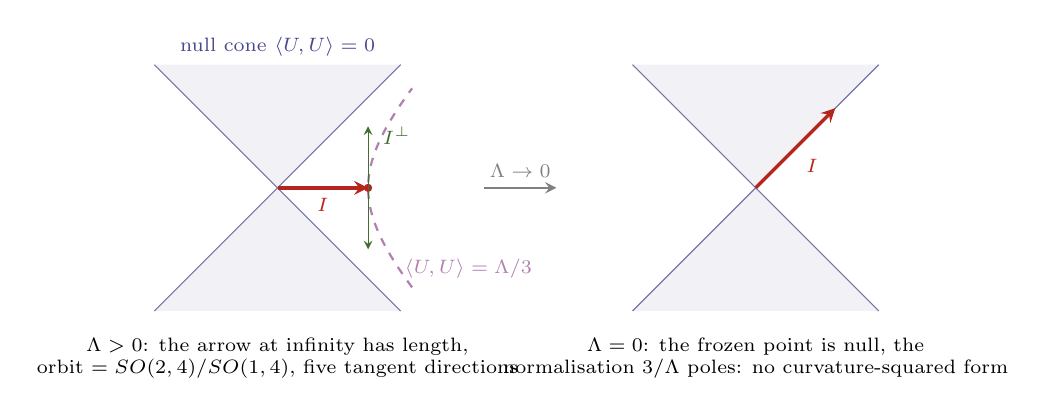
\begin{tikzpicture}[scale=0.92, >=stealth]
% left panel: Lambda > 0
\begin{scope}
  \fill[MidnightBlue!6] (-1.7,1.7) -- (0,0) -- (1.7,1.7) -- cycle;
  \fill[MidnightBlue!6] (-1.7,-1.7) -- (0,0) -- (1.7,-1.7) -- cycle;
  \draw[MidnightBlue!60] (-1.7,-1.7) -- (1.7,1.7);
  \draw[MidnightBlue!60] (-1.7,1.7) -- (1.7,-1.7);
  \node[MidnightBlue!80, font=\scriptsize] at (0,1.95) {null cone $\ip{U}{U} = 0$};
  % the orbit hyperbola through the tip of I
  \draw[dashed, thick, Plum!80!black, domain=-0.95:0.95, samples=60]
    plot ({1.25*cosh(\x)}, {1.25*sinh(\x)});
  \node[Plum!80!black, font=\scriptsize, anchor=west] at (1.62,-1.12)
    {$\ip{U}{U} = \Lambda/3$};
  % the frozen point
  \draw[very thick, ->, BrickRed] (0,0) -- (1.25,0) node[midway, below, font=\scriptsize] {$I$};
  \fill[BrickRed] (1.25,0) circle (1.6pt);
  % Goldstone tangent directions
  \draw[->, OliveGreen!80!black] (1.25,0) -- (1.25,0.85);
  \draw[->, OliveGreen!80!black] (1.25,0) -- (1.25,-0.85);
  \node[OliveGreen!80!black, font=\scriptsize, anchor=west] at (1.32,0.72) {$I^{\perp}$};
  \node[font=\scriptsize, align=center] at (0,-2.35)
    {$\Lambda > 0$: the arrow at infinity has length,\\
     orbit $= SO(2,4)/SO(1,4)$, five tangent directions};
\end{scope}
% arrow between panels
\draw[->, thick, gray] (2.85,0) -- (3.85,0) node[midway, above, font=\scriptsize] {$\Lambda \to 0$};
% right panel: Lambda = 0
\begin{scope}[xshift=6.6cm]
  \fill[MidnightBlue!6] (-1.7,1.7) -- (0,0) -- (1.7,1.7) -- cycle;
  \fill[MidnightBlue!6] (-1.7,-1.7) -- (0,0) -- (1.7,-1.7) -- cycle;
  \draw[MidnightBlue!60] (-1.7,-1.7) -- (1.7,1.7);
  \draw[MidnightBlue!60] (-1.7,1.7) -- (1.7,-1.7);
  % I fallen onto the cone
  \draw[very thick, ->, BrickRed] (0,0) -- (1.1,1.1) node[midway, below right, font=\scriptsize] {$I$};
  \node[font=\scriptsize, align=center] at (0,-2.35)
    {$\Lambda = 0$: the frozen point is null, the\\
     normalisation $3/\Lambda$ poles: no curvature-squared form};
\end{scope}
\end{tikzpicture}
\caption{The existence boundary of Theorem \ref{thm:action}(2) in one fibre of the ambient bundle. Left: for $\Lambda > 0$ the frozen point $I$ lies off the null cone on the orbit $\ip{U}{U} = \Lambda/3$ of fibre vectors $U$; its stabiliser is $SO(1,4)$, and the five tangent directions $I^{\perp}$ are the $I$-half of the nine Goldstone modes of Proposition \ref{prop:goldstone}, all eaten. Right: as $\Lambda \to 0$ the arrow falls onto the null cone and the normalisation $1/\ip{I}{I} = 3/\Lambda$ develops its pole: a null vector cannot normalise the curvature-squared form of the action. The picture is exact, not schematic: the script verifies the norm identity, the pole, and the five-dimensional tangent space in exact arithmetic.}
\label{fig:arrow}
\end{figure}

% === Section 4 (M2): vacate, dark energy, two kinds ===
\section{What the equations vacate, and what cannot evolve}\label{sec:vacate}

\subsection{The equations vacate what the completion fills}\label{subsec:vacate}

\begin{theorem}[The wall's free sector]\label{thm:wallfree}
Let $e$ be a soldering form of corank one at a point, a regular map $TM \to \mathbb{R}^{1,3}$ with a one-dimensional radical $r$ ($e^a(r) = 0$ for every $a$) and cokernel direction $n$ ($n_a e^a = 0$), so that $g_{\mu\nu} = \eta_{ab}e^a_\mu e^b_\nu$ is finite and degenerate (this is the degeneration dual to the sheaf paper's; see Proposition \ref{prop:whichwall}); the image $e(T_xM)$ is a three-dimensional subspace of the frame space, the wall's tangent space, and it may be of any type (Lorentzian, Riemannian, or null). The Einstein-Cartan equations \eqref{eq:ec} are polynomial in $e$, $\omega$ and their derivatives, so polynomiality (Theorem \ref{thm:action}(1)) keeps them meaningful at the point. Choose the normal form $e^a = dx^a$ for $a = 0,1,2$, $e^3 = 0$, so that $r = \partial_3$, $n = \delta^3$, and the wall's tangent space carries the frame indices $0,1,2$; write $K^{a}{}_{b} := \omega^{a}{}_{3\,b}$ and $M_{c\mu} := \tfrac12\,\epsilon_{cab}\,\omega^{ab}{}_{\mu}$ for $a, b, c, \mu \in \{0,1,2\}$, the boost components into the dying frame direction and the dualised tangential connection, and lower and raise their indices with the wall metric $\eta_{ab}$. Then:
\begin{enumerate}
\item[(a)] \emph{(Torsion.)} Regarded as linear conditions on the $24$ components of the torsion, the connection equation has rank $24$ on the invertible region and rank $18$ at the point: three of its components are identities $0 = 0$ and six torsion components are freed, all tangential to the wall (every component with a leg along $r$, and the cokernel component $n_dT^d$, are forced to vanish). Regarded as conditions on the $36$ components of the curvature, the frame equation has rank $16$ in both cases: no curvature condition is lost, and the components of the frame equation along the radical do \emph{not} vanish identically.
\item[(b)] \emph{(Connection.)} Regarded as conditions on the $24$ components of $\omega$, the connection equation has rank $12$ at the point. The free sector is exactly two symmetric tensors on the wall's tangent space: $K_{ab}$ symmetric (six components), which is invisible to the torsion because it multiplies $e^3 = 0$, and $M_{c\mu}$ symmetric (six components), which is the connection image of the freed torsion of (a), $t = (\operatorname{tr}M)\,\mathbf{1} - M$. Forced to their Levi-Civita values are the antisymmetric parts of $K$ and $M$ and every component $\omega^{ab}{}_{3}$ along the radical leg.
\item[(c)] \emph{(Propagation.)} The frame equation contains no derivative of the symmetric part of $M$ in any direction. Its principal symbol in the radical direction determines the radial derivatives $\partial_3 K_{ab}$ of all six components of $K$, and its tangential symbols impose first-order conditions on $K$ along the wall. The field equations therefore cannot propagate $M$ across the wall.
\item[(d)] \emph{(The wall's Hamiltonian constraint.)} In the normal form with $de = 0$, on the free sector $K \oplus M$ the frame equation reduces to a single component, $E_3$ evaluated on $(\partial_0, \partial_1, \partial_2)$, which reads
\[
\sigma_2'(M) \;-\; \sigma_2'(K) \;-\; 2\Lambda \;=\; 0, \qquad \sigma_2'(A) := (\operatorname{tr}A)^2 - \operatorname{tr}(A^2),
\]
with traces taken on the mixed tensors $M^{c}{}_{\mu}$, $K^{a}{}_{b}$: $K$ and $M$ enter only there, only quadratically, and with no cross term; the other fifteen components of the frame equation vanish identically on the free sector. On a curved wall the Levi-Civita part of $\omega$ adds the wall's intrinsic curvature to this component and algebraic cross terms with $M$ and $K$ to the others.
\end{enumerate}
Consequently, on the flat model of (d), the field equations at a corank-one wall of the soldering form determine the connection up to a symmetric bilinear form $M$ on the wall's tangent space which they constrain by one scalar relation and never propagate: data on the wall that the bulk equations do not determine. On a curved wall the statement that survives is (c): $M$ is never propagated; how much of $M$ the fifteen other components then fix algebraically, through their cross terms with the Levi-Civita part and with the first derivatives of the connection, is a jet computation not done here (successor problem (2)). \emph{Level:} proved, for the equations as imported in Fact \ref{fact:mm}; the ranks and symbol ranks are invariant under the changes of frame and coordinates that preserve the normal form. The script confirms in exact arithmetic the counts of (a) to (c) and the single surviving component of (d) for all three types of dying direction, and the $K \oplus M$ description of (b) with the identity of (d) for the Lorentzian and Riemannian types, whose wall metric is nondegenerate; at the Riemannian type, where the boost is into a timelike direction, the cosmological term enters (d) with the opposite sign, $\sigma_2'(K) - \sigma_2'(M) - 2\Lambda = 0$. At the null type the dying direction lies in the wall, the wall metric is degenerate, and the twelve-dimensional free sector does not split as $K \oplus M$; (b) and (d) are stated for the Lorentzian normal form only. Which walls are of this type, and in particular that the sheaf paper's wall is not, is Proposition \ref{prop:whichwall}.
\end{theorem}

\begin{proof}
\emph{Normal form.} Both equations are built from $\epsilon_{abcd}$, $e$, $\omega$ and $d$, without the metric. Under $GL(4)$ on the coordinates and the Lorentz group on the frame, $\epsilon_{abcd}$ is invariant up to $\det$, so ranks and symbol ranks are invariant; a corank-one $e$ may be brought to $e^a = dx^a$ ($a = 0,1,2$), $e^3 = 0$ by a coordinate change and a Lorentz rotation whenever the image is Lorentzian, to $e^0 = 0$ when it is Riemannian, and to $e^0 = e^1 = dx^0$, $e^2 = dx^2$, $e^3 = dx^3$ when it is null; the script runs all three, with identical counts, and the argument below is written for the first. Throughout, a three-form in four variables has four components, one for each omitted coordinate.

\emph{(a) Torsion, pairs not containing $3$.} For $(a,b) \in \{01, 02, 12\}$ the only nonzero terms of $\epsilon_{abcd}\,e^c\wedge T^d$ have $d = 3$, since $e^3 = 0$ removes the terms with $c = 3$; with $c$ the remaining index the equation reads $dx^c\wedge T^3 = 0$. So $T^3\wedge dx^0 = T^3\wedge dx^1 = T^3\wedge dx^2 = 0$. A two-form divisible by $dx^0$ and by $dx^1$ is a multiple of $dx^0\wedge dx^1$, and divisibility by $dx^2$ then forces it to vanish: $T^3 = 0$, six independent conditions. Each of the three equations has one component that is identically zero, the one omitting $c$: three vacated components. \emph{Pairs containing $3$.} For $(a, 3)$ with $\{b, c\} = \{0,1,2\}\setminus\{a\}$ the equation reads $dx^b\wedge T^c = dx^c\wedge T^b$. Split $T^b = \theta^b\wedge dx^3 + \tau^b$ with $\theta^b$ a one-form and $\tau^b$ a two-form in $dx^0, dx^1, dx^2$. The $dx^3$ parts give $dx^b\wedge\theta^c = dx^c\wedge\theta^b$ for all three pairs: writing $\theta^b = \theta^b_\mu dx^\mu$ and $\mu$ for the index other than $b, c$, the components are $\theta^c_\mu = 0$, $\theta^b_\mu = 0$ and $\theta^b_b + \theta^c_c = 0$; over the three pairs every off-diagonal component vanishes and $\theta^0_0 + \theta^1_1 = \theta^0_0 + \theta^2_2 = \theta^1_1 + \theta^2_2 = 0$, so $\theta = 0$: nine conditions, every radical-leg component gone. The $dx^3$-free parts give $dx^b\wedge\tau^c = dx^c\wedge\tau^b$, one condition per pair, three in all, on the nine components of $\tau$: six free, all tangential. Total rank $6 + 9 + 3 = 18$; on the invertible region the same argument with all four $dx^a$ present is the classical one and gives $T = 0$, rank $24$. \emph{Frame equation.} With $e^3 = 0$,
\[
\begin{aligned}
E_3 &= \epsilon_{3bcd}\,dx^b\wedge F^{cd} \qquad (b,c,d \in \{0,1,2\}),\\
E_a &= 2\sum_{b,c}\epsilon_{abc3}\,dx^b\wedge F^{c3} \qquad (a \in \{0,1,2\};\ b, c \in \{0,1,2\}\setminus\{a\}).
\end{aligned}
\]
The unknowns separate: $F^{01}, F^{02}, F^{12}$ enter only $E_3$, and $F^{03}, F^{13}, F^{23}$ enter only $E_0, E_1, E_2$. For $E_3$, the four choices $F^{12} = dx^1\wedge dx^2$, $dx^1\wedge dx^3$, $dx^2\wedge dx^3$ and $F^{02} = dx^2\wedge dx^3$ produce, one each, the four components of a three-form: rank $4$. For $E_0, E_1, E_2$ split $F^{c3} = \phi^c\wedge dx^3 + \psi^c$. The $dx^3$-leg components are $\epsilon_{abc}\,dx^b\wedge\phi^c$, nine from nine, and this map is the $\theta$ system above with the roles renamed, hence bijective; the $dx^3$-free components, one per $E_a$, are hit independently by $\psi^2_{02}$, $\psi^0_{01}$ and $\psi^1_{12}$. Rank $4 + 9 + 3 = 16$, the full target; on the invertible region rank can only be at least as large and the target is sixteen-dimensional. For the radical components, $\iota_r E_a = -\epsilon_{abcd}\,e^b\wedge\iota_r F^{cd}$ is not zero for generic $F$; the script exhibits an integer instance.

\emph{(b) Connection.} An inhomogeneous $de^a$ enters the connection equation only as a source term, which leaves the rank of the linear map $\omega \mapsto \epsilon\,e\wedge T(\omega)$ unchanged, so take $de = 0$: $T^a = \omega^{a}{}_{b}\wedge e^b$. The dying direction: $T^3 = \sum_{b<3}\omega^{3}{}_{b\mu}\,dx^\mu\wedge dx^b$, whose tangential components are the antisymmetric part of $\omega^{3}{}_{b\mu}$ in $(b,\mu)$ and whose radial-leg components are $\omega^{3}{}_{b3}$; $T^3 = 0$ therefore forces the antisymmetric part of $K$ and the three components $\omega^{a3}{}_{3}$ to vanish and leaves the symmetric part of $K$ free, six components; $K$ never enters $T^a$ for $a < 3$, because there it multiplies $e^3 = 0$. The tangential connection: for $a < 3$, $T^a = \omega^{a}{}_{b}\wedge dx^b$ over $b < 3$, so $T^a_{\,3n} = \omega^{a}{}_{n3}$ and the radical-leg condition $\theta = 0$ of (a) forces $\omega^{ab}{}_{3} = 0$, three components; and $T^a_{\,mn} = \omega^{a}{}_{nm} - \omega^{a}{}_{mn}$ for $m,n < 3$ is the classical three-dimensional torsion-contortion map, a bijection of nine-dimensional spaces. Dualising with $\omega^{ab}{}_{\mu} = \epsilon^{abc}M_{c\mu}$ and $t^{a}{}_{d} = \tfrac12\epsilon_{d}{}^{mn}T^a_{\,mn}$, the contraction $\epsilon_{dmn}\epsilon^{amc} = \delta^a_d\delta^c_n - \delta^c_d\delta^a_n$ gives $t = (\operatorname{tr}M)\mathbf{1} - M$, so $t$ is symmetric exactly when $M$ is: the three conditions of (a) are the vanishing of the antisymmetric part of $M$, and the free sector is the symmetric part, six components. Forced: three from each of the antisymmetric part of $K$, the radial-leg $\omega^{a3}{}_{3}$, the radial-leg $\omega^{ab}{}_{3}$ and the antisymmetric part of $M$: rank $12$, free $12$, as claimed.

\emph{(c) Propagation.} The derivative terms of the frame equation are $\epsilon_{abcd}\,e^b\wedge d\omega^{cd}$. For $a = 3$ and $b < 3$ the pair $(c,d)$ is the complement of $b$ in $\{0,1,2\}$, so $\omega^{cd}$ is $\pm M_{b\mu}$: the components of $E_3$ with a $dx^3$ leg are $\partial_3(M_{bx} - M_{xb})$ up to sign, the antisymmetric part only, and the component without a $dx^3$ leg is $\epsilon^{bmn}\partial_m M_{bn}$ up to sign, which vanishes on symmetric $M$. So no derivative of symmetric $M$ appears in $E_3$, and none appears in $E_a$ for $a < 3$, where only $\omega^{c3}$, that is $K$ and its forced complement, occurs. For $K$: the $dx^3$-leg components of $E_a$ ($a < 3$) are $\partial_3 K_{c y}$ with $c$ the index other than $a, b$ and $y \neq b$, which over the two choices of $b$ and the allowed $y$ reach all six components of symmetric $K$; the remaining components carry tangential derivatives of $K$. The script confirms the symbol ranks: $0$ on $M$ in every direction, $6$ on $K$ in the radial direction and $3$ in each tangential direction.

\emph{(d) The Hamiltonian component.} With $de = 0$ and the forced sector at its Levi-Civita value zero, $R^{cd} = \omega^{c}{}_{f}\wedge\omega^{fd}$ and the frame equation is quadratic in $(K, M)$. For $a < 3$ every term of $E_a$ carries $\omega^{c3}$ against $\omega^{3d}$ or a tangential $\omega$, and the $dx^3$-free components need three tangential legs from two one-forms and $dx^b$, which is impossible with $b$ fixed by $a$; the script confirms that all twelve components of $E_a$, $a<3$, vanish identically on the free sector. For $E_3$ on $(\partial_0,\partial_1,\partial_2)$: the $f = 3$ terms give $\epsilon_{3bcd}\,dx^b\wedge\omega^{c}{}_{3}\wedge\omega^{3d} = -\epsilon_{bcd}\,\epsilon^{bxy}K^{c}{}_{x}K^{d}{}_{y} = -\bigl(\delta^x_c\delta^y_d - \delta^x_d\delta^y_c\bigr)K^{c}{}_{x}K^{d}{}_{y} = -\sigma_2'(K)$, and the $f < 3$ terms give, after dualising both factors with $\omega^{cd} = \epsilon^{cdg}M_{g\mu}$, the same contraction on $M$ with the opposite sign, $+\sigma_2'(M)$; cross terms vanish because $\omega^{c}{}_{3}\wedge\omega^{3d}$ and $\omega^{c}{}_{f}\wedge\omega^{fd}$ ($f<3$) lie in different terms. The cosmological term $\ell^{-2}\epsilon_{3bcd}\,e^b\wedge e^c\wedge e^d$ contributes $-6\ell^{-2} = -2\Lambda$ on $(\partial_0,\partial_1,\partial_2)$. The script confirms the identity $E_3(\partial_0,\partial_1,\partial_2) = \sigma_2'(M) - \sigma_2'(K)$ on random elements of the free sector, the vanishing of the cross term, and the coefficient $-6$.
\end{proof}

\subsection{Dark energy cannot evolve: the second registered stance}\label{subsec:w}

\begin{proposition}[$w = -1$ on the vacuum region; the registration, and its condition]\label{prop:w}
Three clauses, at three levels.
\begin{enumerate}
\item[(i)] \emph{(Proved.)} On the Einstein region the frozen point is parallel (Fact \ref{fact:frozen}) and the tractor connection preserves the fibre metric, so $\partial_a\ip{I}{I} = 2\ip{\nabla_a I}{I} = 0$: the norm $\Lambda/3$ cannot vary in space or time. A constant $\Lambda$ enters the Einstein equations as the stress-energy $T^{\Lambda}_{ab} = -(\Lambda/8\pi G)\,g_{ab}$, whose pressure and energy density satisfy $p = -\rho$ identically: $w = -1$.
\item[(ii)] \emph{(Proved.)} Off the Einstein region write $I_g$ again for the scale tractor of a general metric $g$ in its own scale, $I_g = (1, 0, J/4)$ (the object written $I$ above is its Einstein case, $J/4 = \Lambda/6$), with $J = P_a{}^a$ the trace of the Schouten tensor, the slot that makes $I_g$ parallel exactly when $g$ is Einstein (proved below); by \eqref{eq:tractormetric}, $\ip{I_g}{I_g} = J/2 = R/12$, which equals $\Lambda/3$ precisely when $R = 4\Lambda$. On a matter-dominated cosmology $R$ is not constant, so the naive extension of the identification to the epochs at which $w$ is measured does not give a constant.
\item[(iii)] \emph{(Registered, conditional.)} If dark energy is the norm of the frozen point (Theorem \ref{thm:action}), and if the frozen point admits a definition on a matter-filled region that keeps it parallel (successor problem (3) of Section \ref{sec:verdict}), then $w = -1$ exactly, at every epoch, with no evolution and no quintessence. This is a maximally rigid stance in a field of flexible proposals: most dark-energy models add freedom to $\Lambda$CDM, this one removes it. \emph{The confrontation, recorded as of 2026:} the second data release of the Dark Energy Spectroscopic Instrument \cite{DESI2025}, combining baryon-acoustic-oscillation, cosmic-microwave-background and supernova data, reports a preference for an evolving equation of state at roughly three to four standard deviations, with significance depending on the supernova compilation. The preference is contested on three grounds (it concentrates in the derivative of $w$ rather than any mean offset from $-1$; it is prior-sensitive; the driving dataset combinations exhibit internal tensions), so it is not a detection. The framework does not rely on the dispute and states its exposure plainly: a confirmed detection of $w \neq -1$ at any epoch refutes the frozen-point reading of dark energy, with no parameter available to absorb the result. The condition in (iii) is the one way the reading could avoid such a refutation, and the paper names it rather than uses it: a definition of the frozen point off the vacuum region that made the norm track $R/12$ would be refuted already.
\end{enumerate}
\end{proposition}

\begin{proof}
(i) is the displayed computation. (ii): by \eqref{eq:conn}, for $I_g = (1, 0, J/4)$ the $\sigma$ slot of $\nabla_a I_g$ is $0 - 0 = 0$, the $\rho$ slot is $\tfrac14\partial_a J + P_a{}^b\cdot 0 = \tfrac14\partial_a J$, and the $\mu$ slot is $0 + (J/4)g_{ab} - P_{ab}$, minus the trace-free Schouten tensor. The $\mu$ slot vanishes if and only if $P_{ab}$ is pure trace, that is if and only if $g$ is Einstein; and an Einstein four-metric has constant scalar curvature by the contracted Bianchi identity, hence constant $J$, so the $\rho$ slot vanishes with it. Thus $\nabla I_g = 0$ exactly when $g$ is Einstein. The norm is \eqref{eq:tractormetric}: $\ip{I_g}{I_g} = 2\cdot 1\cdot J/4 = J/2$, and $J = R/6$ in four dimensions. The script confirms the $\mu$ slot on an exact non-Einstein instance and on an Einstein one, and the $\rho$ slot $\tfrac14\partial_a J$ on an instance with non-constant $J$. (iii) is a registration, not a computation.
\end{proof}

\subsection{Two kinds of action: the ninth refutation}\label{subsec:twokinds}

\begin{theorem}[Gravity is pre-metric; the forces degenerate exactly where the conformal class does]\label{thm:twokinds}
(Shared with the Standard-Model paper \cite{ButlerT12}, which uses it from the internal side.)
\begin{enumerate}
\item Neither of the two routes by which the MacDowell-Mansouri mechanism could extend to an internal factor is open. Contraction with the frozen point produces nothing there: $I$ is a singlet for the internal group and an internal field strength carries no tractor index, so no invariant of the form $\epsilon(I, \cdot, F_i, F_i)$ exists. And the star-free quadratic invariants of an internal field strength, $\int\tr(F_i\wedge F_i)$ for each simple factor, are topological: a boundary term with vanishing interior variation and no field equations. The natural conjecture, that the forces are gauged polynomially as gravity is, fails along both routes: the ninth refutation in the series' record \cite[Table~1, row 9]{ButlerT17}. (Whether some polynomial functional of a different shape could serve is not decided here.)
\item What exists instead are the Yang-Mills functionals $S_i = (1/2g_i^2)\int \tr(F_i \wedge {*}F_i)$, and the Hodge star on two-forms in four dimensions depends on exactly one piece of metric data, the conformal class $[g]$, and is independent of the scale. The internal forces are therefore \emph{conformal-level} objects, defined exactly where the conformal class is nondegenerate, while gravity's action alone is \emph{pre-metric}: polynomial in the connection, the frozen point and the Stelle-West vector, defined across the singular locus (Theorem \ref{thm:action}(1)).
\item Corollary: at a tame corank-one wall the cometric acquires a radical and the metric a pole (Fact \ref{fact:walls}), so the conformal class degenerates and the star on two-forms, built from two inverse metrics and the volume form, is no longer a nondegenerate map there; the internal actions degenerate with the metric, what crosses is gravity together with the topological $\theta$-terms, the part of each force that survives the singularity.
\end{enumerate}
\end{theorem}

\begin{proof}
(1) Internal invariance of $I$ is structural: $I$ is a section of the tractor factor and the internal groups act on the internal factor, and $F_i$ is a two-form with values in the internal Lie algebra, with no tractor slot for $\epsilon$ or $I$ to contract. Topologicality: $d\,\tr(F\wedge F) = \tr(DF\wedge F) + \tr(F\wedge DF) = 2\tr(DF\wedge F) = 0$ by the Bianchi identity $DF = 0$, using that two-forms commute under the wedge and the trace is cyclic; locally $\tr(F\wedge F) = d(\mathrm{CS}(A))$, and the variation $\delta\int\tr(F\wedge F) = 2\int\tr(D\delta A\wedge F) = 2\int d\,\tr(\delta A\wedge F) - 2\int\tr(\delta A\wedge DF)$ is a boundary term plus zero: no field equations. (2) The star on two-forms in four dimensions is $*\alpha_{ab} = \tfrac12\sqrt{|g|}\,\epsilon_{abcd}\,g^{ce}g^{df}\alpha_{ef}$; under $g \mapsto \Omega^2 g$ the factor $\sqrt{|g|}$ scales by $\Omega^4$ and the two inverse metrics by $\Omega^{-4}$, so $*$ is invariant: it depends on $[g]$ only, and not on the scale that the frozen point fixes. It does depend on $[g]$: with $g$ degenerate, $g^{-1}$ does not exist. (3) is (2) read at a corank-one wall, where the cometric $g^{ce}$ has a one-dimensional radical and $\sqrt{|g|}$ a half-power pole (Fact \ref{fact:walls}), for every representative of the conformal class alike, so $*$ on two-forms is not a nondegenerate map there; the $\theta$-terms $\theta\int\tr(F\wedge F)$ are star-free, hence cross. The trace identities used in (1) are confirmed by the script on exact instances; they are the only computational content.
\end{proof}

\begin{remark}[Point of contact: what the dichotomy explains]\label{rem:dichotomy}
The theorem answers questions it was not asked, and the series keeps them in view per its practice: why gravity is universal (it is the one force whose action needs no metric); why it alone resists quantisation-as-a-force (it was never a force in the sense the others are: its action is pre-metric while theirs are conformal-level); and what survives the singularity (gravity, and the strong-CP parameter, which crosses). What the dichotomy does not determine, and what this paper does not supply: the three coupling normalisations $g_i$, the condensation data, and the chirality of the weak coupling, which are the task of the matter papers, the mass paper T11 \cite{ButlerT11} and the standard-model paper T12 \cite{ButlerT12}.
\end{remark}

\subsection{Which wall: the soldering form against the sheaf paper's degeneration}\label{subsec:whichwall}

Theorem \ref{thm:wallfree} is a theorem about a soldering form with a radical: $g_{\mu\nu} = \eta_{ab}e^a_\mu e^b_\nu$ degenerate, the metric on tangent vectors acquiring a null direction. The sheaf paper's tame wall is a degeneration of the \emph{cometric}, the form on covectors, and the two are not the same degeneration. The following proposition records exactly how they differ, what the sheaf paper's wall looks like in soldering variables, and which piece of the completion the wall's extra freedom is.

\begin{proposition}[The sheaf paper's wall in soldering variables]\label{prop:whichwall}
Let $\Sigma$ be a tame corank-one wall of the sheaf paper \cite[Hyp.~2.1, Thm.~3.1]{ButlerT4}: the cometric $G$ on $T^*M$ has a one-dimensional radical $\mathcal{L}$ spanned by a covector $k$, with transversality datum $\delta$, and the physical metric has the residue $\lim_{\tau\to 0}\tau\, G^{-1} = k\otimes k/T$ of \cite[Thm.~6.2]{ButlerT4}, $T \neq 0$. Then:
\begin{enumerate}
\item[(i)] \emph{(Not a wall of the soldering form.)} Any coframe $e^a$ with $\eta_{ab}e^a e^b = G^{-1}$ has a component of order $\tau^{-1/2}$ along $k$: the soldering form does not acquire a radical at $\Sigma$, it acquires a half-power pole, and it is the frame, the map $\mathbb{R}^{1,3} \to TM$, that degenerates. Theorem \ref{thm:wallfree} does not apply to $\Sigma$ in the physical chart.
\item[(ii)] \emph{(The weighted chart.)} In the sheaf paper's weighted module, where $k$ is rescaled to a regular section, the coframe is regular and of full rank and it is the internal cometric of the frame, $\eta^{ab}(\tau) = G(e^a, e^b)$, that acquires the radical: $\eta^{ab}(0) = \mathrm{diag}(0, \eta_3)$ with $\eta_3$ the nondegenerate form of the three surviving directions. The Lie algebra of frame transformations compatible with the degenerate internal cometric, $\{A \in \mathfrak{gl}(4) : A\eta + \eta A^{\mathsf T} = 0\}$, has dimension seven: the three-dimensional orthogonal algebra of the surviving directions, the three null rotations $m_i \mapsto m_i + v_i k$, and the dilation of the dying line $k \mapsto \alpha k$. Compared with the six-dimensional Lorentz algebra of the invertible region, the wall opens exactly one new gauge generator per point, the dilation of $\mathcal{L}$.
\item[(iii)] \emph{(The dilation is the ladder pair's boost.)} In the ambient fibre $\mathbb{R}^{2,4}$ of the completion, with the four-plane $\mathcal{P} = T^*_x M$ carrying the degenerate form, the radical $k \in \mathcal{P}$, and the Witt partner $k^*$ of \cite[Cor.~4.5]{ButlerT4} ($\ip{k}{k^*} = 1$, $k^*$ null, $k^* \perp \mathcal{P}$ except for $k$), the subalgebra of $\mathfrak{so}(2,4)$ preserving $\mathcal{P}$ has dimension eight and restricts onto the full seven-dimensional algebra of (ii). The dilation of $\mathcal{L}$ lifts to the element $k \mapsto \alpha k$, $k^* \mapsto -\alpha k^*$, fixing the surviving directions: the $\mathfrak{so}(1,1)$ boost of the ladder plane $\mathrm{span}(k, k^*)$, which is the rescaling $k \mapsto ck$, $k^* \mapsto k^*/c$ that the sheaf paper's residue theorem identifies as the freedom of the partner line. The one gauge generator the wall opens is the one-parameter group of the ladder pair.
\item[(iv)] \emph{(Dichotomy for the dynamics.)} Wherever the MacDowell-Mansouri datum of Theorem \ref{thm:action} is regular and its soldering form $e = \nabla V$ has full rank, the Einstein-Cartan equations have full rank (Theorem \ref{thm:wallfree}(a) on the invertible region): nothing is vacated. Wherever $e$ is regular of corank one, Theorem \ref{thm:wallfree} applies and the free sector is the symmetric form $M$. At the sheaf paper's wall, in the tractor chart $e$ has a pole and neither case applies; in the sheaf paper's own ambient chart the question is whether the datum $(\nabla, I, V)$, $V = X - (3/\Lambda)I$, extends regularly across $\Sigma$ with $\nabla X$ of full rank, which is the interface the sheaf paper itself flags in its tractor dictionary and poses among its successor problems \cite[\S 7.3-7.4]{ButlerT4}. For the Schwarzschild wall the answer is now known, and it is the second of the two answers just named, in a precise form: the datum has a simple pole whose residues are the completion's weights (Proposition \ref{prop:kasnerwall}, Assembly \ref{asm:forcing}).
\end{enumerate}
\emph{Level:} (i)-(iii) proved, on the imported residue theorem and Witt partner; (iv) is a statement of cases, each case proved, with the case that obtains at the sheaf paper's wall open.
\end{proposition}

\begin{proof}
(i) Write $r$ for a tangent vector with $k(r) = 1$. By the residue, $G^{-1}(r, r) = \tau^{-1}/T + O(1)$, so $\eta_{ab}\,e^a(r)\,e^b(r) = \tau^{-1}/T + O(1)$, and at least one $e^a(r)$ is of order $\tau^{-1/2}$. The frame $E_a$ dual to $e^a$ then has $k(E_a) = O(\tau^{1/2})$ for that $a$: its image collapses into $\ker k$ at $\tau = 0$. A soldering form with a radical would have $g_{\mu\nu}$ finite and degenerate; here $g_{\mu\nu}$ is infinite in one direction. (ii) In the weighted module the Gram of the coframe is the matrix $G(\tau)$ of \cite[proof of Thm.~6.2]{ButlerT4}, $\begin{psmallmatrix}\lambda & b^{\mathsf T}\\ b & G_1\end{psmallmatrix}$ with $\lambda(0) = b(0) = 0$ and $G_1(0)$ invertible: that is $\eta^{ab}(0) = \mathrm{diag}(0, \eta_3)$. For the stabiliser write $A = \begin{psmallmatrix}\alpha & u^{\mathsf T}\\ v & B\end{psmallmatrix}$; then $A\eta + \eta A^{\mathsf T} = \begin{psmallmatrix} 0 & u^{\mathsf T}\eta_3\\ \eta_3 u & B\eta_3 + \eta_3 B^{\mathsf T}\end{psmallmatrix}$, which vanishes if and only if $u = 0$ and $B \in \mathfrak{so}(\eta_3)$, with $\alpha$ and $v$ free: $1 + 3 + 3 = 7$. (iii) Take the ambient basis $(k, m_1, m_2, m_3, k^*, w)$ with $\ip{k}{k^*} = 1$, $\ip{m_i}{m_j} = (\eta_3)_{ij}$, $\ip{w}{w} = +1$ and all other products zero, which has signature $(2,4)$ for $\eta_3$ negative definite. An element of $\mathfrak{so}(2,4)$ preserving $\mathcal{P} = \mathrm{span}(k, m_i)$ preserves $\mathcal{P}^\perp = \mathrm{span}(k, w)$; solving the linear conditions gives an eight-dimensional algebra whose restriction to $\mathcal{P}$ is the seven-dimensional algebra of (ii) (the one-dimensional kernel acts on $\mathrm{span}(k^*, w)$ alone). The element restricting to $\mathrm{diag}(\alpha, 0, 0, 0)$ on $\mathcal{P}$ is forced by $\ip{k}{k^*} = 1$ to send $k^* \mapsto -\alpha k^*$ and, by orthogonality, to fix $w$: it is the boost of the hyperbolic plane $\mathrm{span}(k, k^*)$. The script verifies both dimensions, the surjectivity of the restriction, and the lift of the dilation as exact matrices. (iv) The first case is Theorem \ref{thm:wallfree}(a) on the invertible region (rank $24$ and $16$); the second is Theorem \ref{thm:wallfree}; the third is (i) together with the identification $e = \nabla X$ of Lemma \ref{lem:sw}, whose Gram in the tractor chart is the physical metric $g_{\mu\nu}$, which has the pole.
\end{proof}

\begin{remark}[What this settles, and what it reformulates]\label{rem:whichwall}
Two things are settled. The symmetric form $M$ of Theorem \ref{thm:wallfree} is the free sector of a wall of the soldering form, the degeneration dual to the sheaf paper's, and it is not the completion's sector at the sheaf paper's wall; the claim that the sheaf paper's wall is a wall of the soldering form is withdrawn. And the completion's ladder pair does appear in the dynamics at the sheaf paper's wall, but as gauge, not as a field: the wall opens exactly one new gauge generator per point, the dilation of the dying line, and that generator is the boost of the ladder plane $\mathrm{span}(k, k^*)$. The half-power weight that the sheaf paper's residue theorem assigns to $k$ ($\mathcal{L}^{\otimes 2} \cong N^*\Sigma$) is a particular gauge choice for this generator, the one that makes the exceptional algebra nondegenerate. What is reformulated is the dynamical question: whether the equations demand the completion becomes, at the sheaf paper's wall, the question of how the MacDowell-Mansouri datum fails to extend, and Section \ref{subsec:kasner} answers it for the Schwarzschild wall: the datum's connection has a simple pole, and the residues of that pole are the weights from which the completion is built.
\end{remark}

\subsection{The interface at the Schwarzschild wall: the datum has a pole, and its residue is the completion's weight}\label{subsec:kasner}

Proposition \ref{prop:whichwall}(iv) left one question: whether the MacDowell-Mansouri datum $(\nabla, I, X)$ extends regularly across the sheaf paper's wall. For the Schwarzschild singularity the geometry and sheaf papers between them already contain the answer, and this subsection extracts it and computes what it does to the action.

\begin{fact}[Imported: the weighted limit at the Schwarzschild singularity, and its matching]\label{fact:weightedlimit}
In the Schwarzschild interior in synchronous time $\tau$ (with $\tau = 0$ the singularity), and equally in the Schwarzschild-de Sitter interior, whose metric functions differ by relative $O(\Lambda\tau^2)$ and for which the same limit holds with the same exponents and rates \cite[Thm.~5.9]{ButlerT6}, the orthonormal frame adapted to the Killing and sphere directions is parallel along $\partial_\tau$, and its connection is Kasner at leading order: the Hubble-normalised connection $\tau\,\omega$ tends to $\sum_i p_i\, B_i \otimes \hat\theta^i$ with $B_i$ the boosts, $\hat\theta^i$ the normalised coframe, and exponents $(p_1, p_2, p_3) = (-\tfrac13, \tfrac23, \tfrac23)$, with explicit rates: $O(\tau^{2/3})$ in the boost block and $O(\tau^{1/3})$ in the rotation block, the latter being the sphere's own connection, which is outside the Kasner comparison; the limit is a values-level statement (the algebra generated by the limiting connection values); the transport-level statement, convergence of the transport to the Kasner model's transport, holds along every tangential curve of fixed Hubble-normalised length, for every admissible metric of the geometry paper's class \cite[Def.~5.5]{ButlerT6}, whose exponents satisfy $\sum_i p_i^2 = 1$ \cite[Thm.~5.11]{ButlerT6}, and along the Schwarzschild $\varphi$-lines exactly, at rate $\tau^{1/3}$ \cite[Cor.~5.12]{ButlerT6}; what the geometry paper disclaims is the comparison over segments of fixed coordinate length, whose Hubble-normalised length diverges, and about which no claim is made here either. This coframe consists of sections of the sheaf paper's exceptional module, the weights of the sheaf paper's completion are forced to equal the exponents, and the total residue bivector $B_w = \sum_i p_i\, \hat e_0\wedge\hat e_i$ is a unit boost of the exceptional algebra. \emph{Provenance:} \cite[Lems.~5.1-5.4, Def.~5.5, Thm.~5.6, Thm.~5.9, Thm.~5.11, Cor.~5.12]{ButlerT6}; \cite[Thm.~8.16, Prop.~8.26, Thm.~8.27]{ButlerT4}.
\end{fact}

\begin{proposition}[The cosmological constant does not change the residue]\label{prop:lambdacorr}
Let $g = d\tau^2 - \sum_i a_i(\tau)^2(dx^i)^2$ be a diagonal Bianchi I metric with Hubble rates $H_i = \dot a_i/a_i$, so that the Levi-Civita connection is $\omega^{i0} = H_i\,e^i$, and impose the Einstein equations with cosmological constant, $\mathrm{Ric} = \Lambda g$:
\[
\dot H_i + H_i\sum_j H_j = \Lambda \quad (i = 1,2,3), \qquad \sum_{i<j}H_iH_j = \Lambda .
\]
Then for every Kasner point $(p_1, p_2, p_3)$ there is a unique formal solution with a simple pole of residue $p$ at $\tau = 0$, and it is odd in $\tau$ with regular corrections:
\[
H_i \;=\; \frac{p_i}{\tau} \;+\; \frac{\Lambda}{2}\,(1 - p_i)\,\tau \;+\; \sum_{n \geq 2} h_{i,n}\,\tau^{2n-1},
\]
every $h_{i,n}$ a polynomial in $\Lambda$ and $p$ determined by the evolution equations alone, the constraint then holding identically. In the Bianchi I class the first correction to the connection is therefore $O(\Lambda\tau)$ and regular. At a Schwarzschild-de Sitter wall, whose slices are Kantowski-Sachs rather than flat, the sphere's intrinsic curvature adds corrections of relative order $\tau^{1/3}$ in the rotation block and $\tau^{2/3}$ in the boost block (Fact \ref{fact:weightedlimit}), larger than $\Lambda\tau^2$ and singular in absolute terms; what this proposition establishes there is only that the residue, the coefficient of $\tau^{-1}$, is the Kasner boost of the $\Lambda = 0$ approach and that the field equations at the wall remain the Kasner relations.
\end{proposition}

\begin{proof}
Substitute $H_i = p_i/\tau + \sum_{n\geq 1}h_{i,n}\tau^{2n-1}$. At order $\tau^{-2}$ the evolution equations give $-p_i + p_i\sum_j p_j = 0$ and the constraint gives $\sum_{i<j}p_ip_j = 0$: the Kasner relations. At order $\tau^{2n-2}$, $n \geq 1$, the evolution equation for $i$ reads $(2n-1)h_{i,n} + h_{i,n}\sum_j p_j + p_i\sum_j h_{j,n} = \Lambda\,\delta_{n,1} - K_{i,n}$, where $K_{i,n}$ collects the products of coefficients already determined; with $\sum p = 1$ this is $2n\,h_{i,n} + p_i\,\mathcal{H}_n = \Lambda\delta_{n,1} - K_{i,n}$ with $\mathcal{H}_n := \sum_j h_{j,n}$. Summing over $i$ gives $(2n+1)\mathcal{H}_n = 3\Lambda\delta_{n,1} - \sum_iK_{i,n}$, which determines $\mathcal{H}_n$ and then each $h_{i,n}$ uniquely. For $n = 1$, $K_{i,1} = 0$, so $\mathcal{H}_1 = \Lambda$ and $h_{i,1} = (\Lambda - p_i\Lambda)/2$. Odd powers only: no even power of $\tau$ is sourced, since the equations are quadratic in $H$ with the pole at odd order and $\Lambda$ at order zero. The constraint is preserved by the evolution: with $S := \sum_iH_i$ and $C := \sum_{i<j}H_iH_j$ the evolution equations give $\dot C = 2S(\Lambda - C)$, so $C - \Lambda$ obeys a linear homogeneous equation whose solutions near $\tau = 0$ behave as $\tau^{-2}$, and the Kasner relation $\sum_{i<j}p_ip_j = 0$ sets that mode's coefficient to zero; the constraint therefore holds to all orders once it holds at the pole. Odd powers only is likewise forced: an even power $c_i\tau^{2n}$ in $H_i$, $n \geq 0$, would enter the evolution equations at order $\tau^{2n-1}$, where nothing sources it, through three terms, $2n\,c_i$ from $\dot H_i$, $c_i\sum_jp_j = c_i$ from $c_i\tau^{2n}$ against the pole of $\sum_jH_j$, and $p_i\sum_jc_j$ from the pole of $H_i$ against $\sum_jc_j\tau^{2n}$; the system $(2n+1)c_i + p_i\sum_jc_j = 0$ sums to $(2n+2)\sum_jc_j = 0$, hence $\sum_jc_j = 0$ and $c_i = 0$; the script confirms this by direct substitution to order $\tau^4$ at the Schwarzschild exponents with $\Lambda = 3$, where $h_{i,1} = (2, \tfrac12, \tfrac12)$, $h_{i,2} = (-\tfrac{33}{20}, -\tfrac{3}{40}, -\tfrac{3}{40})$, and both residuals vanish identically through the order computed. The Schwarzschild-de Sitter interior is not in this class (its slices are Kantowski-Sachs); what the geometry paper's Theorem 5.9 \cite[Thm.~5.9]{ButlerT6} gives is that it shares the residue and the exponents of the Schwarzschild approach, with the same weighted limit and rates, which is all the statement claims for it.
\end{proof}

\begin{proposition}[The frozen-point datum at a Kasner wall]\label{prop:kasnerwall}
Let $g = d\tau^2 - \sum_i a_i(\tau)^2(dx^i)^2$ be a solution of the Einstein equations with cosmological constant $\Lambda \neq 0$ in the diagonal Bianchi I class of Proposition \ref{prop:lambdacorr}, with residue $(p_1,p_2,p_3)$ at $\tau = 0$ and $p_1p_2p_3 \neq 0$ (which excludes exactly the permutations of $(1,0,0)$, the flat Milne point, where every curvature below vanishes and the pole is a coordinate horizon), so that $a_i = \tau^{p_i}(1 + O(\Lambda\tau^2))$ and the Kasner metric $d\tau^2 - \sum_i\tau^{2p_i}(dx^i)^2$ is its leading term; let $e^0 = d\tau$, $e^i = a_i\,dx^i$ be the orthonormal coframe, and let the ambient datum be that of Theorem \ref{thm:action}: $I = (1, 0, \Lambda/6)$, $X = (0,0,1)$, and $\nabla$ the tractor connection \eqref{eq:conn} of $g$, whose Schouten tensor is $P_{ab} = (\Lambda/6)g_{ab}$ because $g$ is Einstein. (An exact Kasner metric is Ricci-flat and carries the null frozen point of $\Lambda = 0$. The statements of (i) and (ii) and the Gauss-Bonnet density of (iii) are computed on the leading Kasner term, with $\Lambda$ entering only through the Schouten summand, and hold verbatim for the exact Kasner metric at $\Lambda = 0$, the Schwarzschild exponents included; $\Lambda \neq 0$ is needed only for the statements about the curvature-squared form of the action, which are made on the Einstein family.) Then, in the orthonormal frame, which for the Schwarzschild-de Sitter interior is the sheaf paper's exceptional chart (Fact \ref{fact:weightedlimit} with Proposition \ref{prop:lambdacorr}), at leading order in $\tau$:
\begin{enumerate}
\item[(i)] \emph{(What is regular, and what is not.)} $I$ and $X$ are constant sections of constant norm, the soldering form $\nabla_a X = e_a$ is regular of full rank, and the soldering and Schouten summands of $\nabla$ are the constant matrices $\eta_{ab}$ and $(\Lambda/6)\eta_{ab}$. The only singular part of the datum is the Levi-Civita block, and its leading term is a simple pole:
\[
\omega^{i0} \;=\; \frac{p_i}{\tau}\, e^i, \qquad \omega^{ij} = 0 ,
\]
with residue the bivector-valued one-form $\sum_i p_i\,B_i\otimes \hat e^i$, $B_i = e_0\wedge e_i$, whose legs are tangential to the wall. It is not a gauge pole: its curvature is a double pole,
\[
R^{i0} \;=\; \frac{p_i(p_i - 1)}{\tau^2}\, e^0\wedge e^i, \qquad R^{ij} \;=\; -\frac{p_i p_j}{\tau^2}\, e^i\wedge e^j .
\]
The datum therefore does not extend regularly across the wall in this chart, and in no chart: the Euler density of (iii) equals $\sqrt{|g|}$ times the Kretschmann scalar on an Einstein metric, because $-4R_{ab}R^{ab} + R^2 = -16\Lambda^2 + 16\Lambda^2 = 0$, so the Kretschmann scalar is $-16p_1p_2p_3\tau^{-4}$ at leading order, divergent when $p_1p_2p_3 \neq 0$, and a curvature scalar is chart-independent.
\item[(ii)] \emph{(The field equations at the wall are conditions on the residue.)} In the curvature convention of the geometry paper, in which de Sitter has $\mathrm{Ric}_{ab} = \Lambda g_{ab}$ and $P_{ab} = (\Lambda/6)g_{ab}$ (the convention that makes $I$ parallel), the Ricci tensor in the frame is diagonal with
\[
\tau^2 R_{00} = \sum_i p_i^2 - \sum_i p_i, \qquad \tau^2 R_{ii} = -\,p_i\Bigl(\sum_j p_j - 1\Bigr) ,
\]
so the vacuum equations at leading order are exactly the Kasner relations $\sum_i p_i = 1 = \sum_i p_i^2$; the second says that the residue bivector $B_w = \sum_i p_i B_i$ is a unit boost. With $\Lambda$ the Einstein-$\Lambda$ system of Proposition \ref{prop:lambdacorr} replaces Ricci-flatness at relative order $\Lambda\tau^2$ and does not affect the residue.
\item[(iii)] \emph{(The action at the wall.)} On the Kasner approach the three terms of Theorem \ref{thm:action}(2) have densities
\[
\begin{aligned}
\epsilon_{abcd}R^{ab}\wedge R^{cd} &= -16\,p_1p_2p_3\;\tau^{-3}\, d\tau\wedge d^3x, \\
\epsilon_{abcd}\,e^a e^b R^{cd} &= O(\Lambda\,\tau)\, d\tau\wedge d^3x, \qquad
\epsilon_{abcd}\,e^ae^be^ce^d = 24\,\tau\, d\tau\wedge d^3x .
\end{aligned}
\]
For the Schwarzschild-de Sitter exponents $p_1p_2p_3 = -4/27$ and the first density is $\tfrac{64}{27}\tau^{-3}$ (for Schwarzschild itself, $\Lambda = 0$, this is the divergence of the bare Gauss-Bonnet integrand, $\sqrt{|g|}$ times the Kretschmann scalar $64/(27\tau^4)$): the curvature-squared form of the action diverges at the wall as $\tau^{-2}$, through the topological term alone, which is exact and contributes nothing to the field equations; the Einstein-Cartan and cosmological terms are finite. The value of the frozen-point action is not defined at the singularity; its variational principle is, and its equations reach the wall as the residue conditions of (ii).
\end{enumerate}
\emph{Level:} (i)-(iii) proved by the displayed computations on the leading Kasner term, which the script confirms in exact arithmetic at two rational Kasner points and one non-Kasner point (where the Ricci tensor is confirmed nonzero), with the $\Lambda$-corrections controlled by Proposition \ref{prop:lambdacorr}; the script also runs the excluded point $(1,0,0)$ and confirms that every curvature coefficient and the Gauss-Bonnet density vanish there, so the hypothesis $p_1p_2p_3 \neq 0$ is needed. The application to the Schwarzschild and Schwarzschild-de Sitter interiors is through Fact \ref{fact:weightedlimit}; the Kantowski-Sachs sphere adds its own relative corrections, $O(\tau^{1/3})$ in the rotation block and $O(\tau^{2/3})$ in the boost block, which do not reach the residue.
\end{proposition}

\begin{proof}
(i) $de^i = p_i\tau^{p_i-1}d\tau\wedge dx^i = (p_i/\tau)\,e^0\wedge e^i$ and $de^0 = 0$. With $\omega^{i0} = (p_i/\tau)e^i$ and $\omega^{ij} = 0$: $de^i + \omega^{i}{}_{0}\wedge e^0 = (p_i/\tau)(e^0\wedge e^i + e^i\wedge e^0) = 0$ and $de^0 + \omega^{0}{}_{i}\wedge e^i = \sum_i (p_i/\tau)\, e^i\wedge e^i = 0$, so this is the Levi-Civita connection. The tractor connection \eqref{eq:conn} adds the soldering summand, $\mu_b \mapsto g_{ab}\rho$, and the Schouten summand, $\mu_b \mapsto -P_{ab}\sigma$, both constant in the orthonormal frame on the Einstein region, and acts on $I$ and $X$ through them: $\nabla_a X = e_a$ and $\nabla I = 0$, regular. Curvature: $R^{i0} = d\omega^{i0} + \omega^{i}{}_{j}\wedge\omega^{j0} = d\bigl(p_i\tau^{p_i-1}dx^i\bigr) = p_i(p_i-1)\tau^{p_i-2}\,d\tau\wedge dx^i$, and $R^{ij} = \omega^{i}{}_{0}\wedge\omega^{0j} = (p_i/\tau)e^i\wedge(-(p_j/\tau)e^j)$. A gauge pole $D\,d\tau/\tau$ has $d(d\tau/\tau) = 0$ and contributes to the curvature only through $(d\tau/\tau)\wedge[D, \omega_{\mathrm{reg}}]$, a simple pole at most; a double pole with tangential legs is not of that form. (ii) With $R^{ab}{}_{cd}$ read off from (i), the contraction $\mathrm{Ric}_{bd} = -R^{a}{}_{bad}$, which is the one that gives de Sitter $\mathrm{Ric} = +\Lambda g$ in the mostly-minus signature, yields $R_{00} = \sum_i p_i(p_i-1)/\tau^2$ and $R_{ii} = -\bigl(p_i(p_i-1) + p_i\sum_{j\neq i}p_j\bigr)/\tau^2 = -p_i(\sum_j p_j - 1)/\tau^2$, off-diagonal terms vanishing because every $R^{ab}$ is a multiple of $e^a\wedge e^b$. (The opposite contraction negates both displays and would give de Sitter $\mathrm{Ric} = -\Lambda g$, inconsistent with $P_{ab} = (\Lambda/6)g_{ab}$ and with the system of Proposition \ref{prop:lambdacorr}, whose de Sitter limit is $3H^2 = \Lambda$.) Vanishing of $R_{ii}$ for some $p_i \neq 0$ gives $\sum p = 1$, and then $R_{00} = 0$ gives $\sum p^2 = 1$. The unit-boost reading is \cite[Prop.~8.26(3)]{ButlerT4}: $B_w$ squares to $\sum p_i^2$ on its boost plane. With $\Lambda$ the corrections are those of Proposition \ref{prop:lambdacorr}, of relative order $\Lambda\tau^2$. (iii) Write $R^{0i} = A_i\,e^0\wedge e^i$, $R^{jk} = C_{jk}\,e^j\wedge e^k$ with $A_i = -p_i(p_i-1)/\tau^2$, $C_{jk} = -p_jp_k/\tau^2$. In $\epsilon_{abcd}R^{ab}\wedge R^{cd}$ the pairs $\{a,b\} = \{0,i\}$, $\{c,d\} = \{j,k\}$ and their exchange each contribute four equal terms, so the sum is $8\sum_i A_iC_{jk}\,e^0e^1e^2e^3 = 8\,p_1p_2p_3\sum_i(p_i - 1)\,\tau^{-4}\,\mathrm{vol}$, and $\sum_i(p_i - 1) = 1 - 3 = -2$ on the Kasner relations; with $\mathrm{vol} = \tau^{\sum p_i}d\tau\wedge d^3x = \tau\,d\tau\wedge d^3x$ this is $-16\,p_1p_2p_3\,\tau^{-3}d\tau\wedge d^3x$. (On the leading Kasner term this equals $\sqrt{|g|}$ times the Kretschmann scalar, $64/(27\tau^4)$ for the Schwarzschild exponents, as it must on an Einstein metric.) The Einstein-Cartan density is $-2\sqrt{|g|}\,R$ up to the fixed normalisation, which vanishes on a vacuum and equals $-8\Lambda\tau$ on the Einstein region; the cosmological density is $4!\,\mathrm{vol}$. Exactness of the first term is Theorem \ref{thm:action}(2).
\end{proof}

\begin{assembly}[The forcing half at the Schwarzschild wall, in the residue sense]\label{asm:forcing}
The steps, each with its provenance:
\begin{enumerate}
\item \emph{(The datum's pole.)} At the Schwarzschild singularity the frozen-point datum is regular in the exceptional chart except for a simple pole of the connection with tangential legs, residue $\sum_i p_iB_i\otimes\hat e^i$: Proposition \ref{prop:kasnerwall}(i) on the Kasner model, transported to Schwarzschild by Fact \ref{fact:weightedlimit} (the geometry paper's weighted limit, values-level, with its $O(\tau^{2/3})$ corrections in the boost block and $O(\tau^{1/3})$ in the rotation block).
\item \emph{(The residues satisfy the wall's field equations.)} The exponents obey the Kasner relations, which are the leading-order field equations, and the second relation is the statement that the residue bivector is a unit boost: Proposition \ref{prop:kasnerwall}(ii), \cite[Prop.~8.26(3)]{ButlerT4}.
\item \emph{(The residues are the completion's weights.)} The sheaf paper's completion at this wall is built on weights that are forced, once the dying direction is named, to equal the Kasner exponents: \cite[Thm.~8.16]{ButlerT4}; and its exceptional frame is the frame in which (1) holds: \cite[Thm.~8.27]{ButlerT4}.
\end{enumerate}
Consequently, at this wall, the field equations neither merely permit the completion nor demand it as a further condition: their own singularity supplies the data the completion is built from. The pole of the dynamical connection is not removable (step 1), its residues are fixed by the equations (step 2), and those residues are the weights of the completion (step 3). This is the forcing half of Section \ref{sec:vacate} answered in the residue sense. Three qualifications are discharged below: the cosmological corrections leave the residue unchanged (Proposition \ref{prop:lambdacorr}); the divergent curvature-squared \emph{value} is removed by a local wall counterterm that does not change the equations (Proposition \ref{prop:counterterm}); and the residue statement holds pointwise for variable exponents in the diagonal class (Lemma \ref{lem:varexp}), with the momentum constraints and the non-diagonal class remaining as the dynamical half of the sheaf paper's connection-level matching \cite[Rem.~8.28]{ButlerT4}.
\end{assembly}

The two remaining qualifications carried by Assembly \ref{asm:forcing} are now discharged in turn: the divergent value, and the variable-exponent class.



\begin{proposition}[The wall counterterm]\label{prop:counterterm}
Assume $\Lambda \neq 0$, so that the curvature-squared form exists. Let $Q(\omega) := \epsilon_{abcd}\bigl(\omega^{ab}\wedge d\omega^{cd} + \tfrac23\,\omega^{ab}\wedge\omega^{c}{}_{e}\wedge\omega^{ed}\bigr)$ be the Chern-Simons three-form of the Lorentz connection for the invariant $\epsilon_{abcd}$. Then:
\begin{enumerate}
\item[(i)] $dQ = \epsilon_{abcd}R^{ab}\wedge R^{cd}$ identically: the topological term of Theorem \ref{thm:action}(2) is exact, with $Q$ as primitive.
\item[(ii)] On a Kasner approach the restriction of $Q$ to the slice $\Sigma_\varepsilon = \{\tau = \varepsilon\}$ is
\[
Q\big|_{\Sigma_\varepsilon} \;=\; 8\,p_1p_2p_3\;\varepsilon^{-2}\, d^3x ,
\]
so that the divergent part of the curvature-squared action on $\{\tau > \varepsilon\}$ is $-\tfrac{3}{\Lambda}\int_{\Sigma_\varepsilon}Q = -\tfrac{24}{\Lambda}\,p_1p_2p_3\,\varepsilon^{-2}\,\mathrm{Vol}_3$, exactly the integral of Proposition \ref{prop:kasnerwall}(iii).
\item[(iii)] The functional $S_{\mathrm{ren}} := S + \tfrac{3}{\Lambda}\int_{\Sigma_\varepsilon}Q(\omega)$, the action with the Chern-Simons form of the connection restricted to the wall added on the wall, has the same interior field equations as $S$ (a boundary term changes the boundary conditions of the variational problem, not the Euler-Lagrange equations), is finite as $\varepsilon \to 0$ on the Kasner approach, and its limit is the Einstein-Cartan and cosmological contributions together with the value of $Q$ on the far boundary. The counterterm is local, but it is not intrinsic to the wall: on the Kasner approach the whole surviving value comes from the cubic term in the boost block $\omega^{i0}$, the extrinsic curvature of the slice, the quadratic term vanishing because every nonzero $\omega^{ab}$ carries the index $0$ and $\epsilon_{abcd}$ needs four distinct indices. And $Q$ is a Chern-Simons form, not gauge invariant: under a local Lorentz rotation of the frame on the slice it shifts by an exact form and a Wess-Zumino term, so the counterterm is defined relative to a frame, here the exceptional frame of Fact \ref{fact:weightedlimit}. The residual ambiguity of the renormalisation is that frame choice together with the $O(\Lambda)$ constant by which the finite part shifts under the corrections of Proposition \ref{prop:lambdacorr}.
\end{enumerate}
On the Kasner approach the counterterm's coefficient $8p_1p_2p_3$ is the third elementary symmetric function of the residue, the one Kasner invariant beyond the two relations.
\end{proposition}

\begin{proof}
(i) is the transgression formula for a quadratic invariant polynomial, here $\epsilon_{abcd}$ on $\mathfrak{so}(1,3)$: $d(\omega\,d\omega) = d\omega\wedge d\omega$ and $d(\omega^3) = 3\,d\omega\wedge\omega^2$ under the invariant pairing, so $dQ = \epsilon(d\omega + \omega^2, d\omega + \omega^2)$ up to the term $\epsilon(\omega^2,\omega^2)$, which vanishes by the invariance of $\epsilon_{abcd}$ under the adjoint action (the Jacobi identity). The script confirms $dQ = \epsilon_{abcd}R^{ab}\wedge R^{cd}$ as an exact identity of forms on the Kasner connection. (ii) On the slice only the terms of $Q$ without a $d\tau$ leg survive. The quadratic term vanishes on the slice for two reasons, either sufficient: every $d\omega^{cd}$ carries a $d\tau$ leg (the connection depends on $\tau$ only and has tangential legs), and every nonzero $\omega^{ab}$ carries the index $0$ while $\epsilon_{abcd}$ needs four distinct indices; and the cubic term reduces to $\tfrac23\epsilon_{i0jk}\,\omega^{i0}\wedge\omega^{j}{}_{0}\wedge\omega^{0k}$ and its index rearrangements: with $\omega^{i0} = (p_i/\tau)e^i$ each is a multiple of $p_1p_2p_3\tau^{-3}e^1\wedge e^2\wedge e^3 = p_1p_2p_3\tau^{-2}d^3x$, and collecting the signs and multiplicities gives the coefficient $8$; the script computes the $(x,y,z)$ component of $Q$ exactly and finds $8p_1p_2p_3\tau^{-2}$. Then $\int_{\tau>\varepsilon}\epsilon RR = \int Q\big|_{\text{far}} - \int_{\Sigma_\varepsilon}Q$ by Stokes, and $-\tfrac3\Lambda\cdot 8p_1p_2p_3\varepsilon^{-2}$ integrates $-\tfrac{3}{\Lambda}\cdot 16 p_1p_2p_3\int_\varepsilon\tau^{-3}d\tau$, matching Proposition \ref{prop:kasnerwall}(iii). (iii) A boundary term does not change the Euler-Lagrange equations in the interior. By (ii) the added term cancels the wall boundary contribution of the exact topological term identically on the Kasner approach, leaving the far-boundary value of $Q$, the Einstein-Cartan term ($2\int\epsilon_{abcd}e^ae^bR^{cd}$, whose density is $-8\Lambda\tau$ on the Einstein region) and the cosmological term ($\tfrac{\Lambda}{3}\int\epsilon_{abcd}e^ae^be^ce^d$, whose density is $24\tau$ before the prefactor), all finite as $\varepsilon\to 0$. With the corrections of Proposition \ref{prop:lambdacorr}, $\omega^{i0} = (p_i/\tau + \tfrac{\Lambda}{2}(1-p_i)\tau + \dots)e^i$ and the cubic term of $Q$ on the slice acquires, beyond $8p_1p_2p_3\tau^{-2}$, a term of order $\Lambda\tau^0$ and higher: a finite constant, which is the only freedom in the subtraction.
\end{proof}

\begin{lemma}[Variable exponents: the residue is pointwise, the corrections are subleading]\label{lem:varexp}
Let $g = d\tau^2 - \sum_i\tau^{2p_i(x)}(dx^i)^2$ with smooth exponents $p_i(x)$ taking values in the open Kasner circle ($\sum p_i = 1 = \sum p_i^2$, all $p_i < 1$), and let $e^0 = d\tau$, $e^i = \tau^{p_i(x)}dx^i$. Then the Levi-Civita connection is
\[
\omega^{i0} \;=\; \frac{p_i(x)}{\tau}\,e^i, \qquad
\omega^{ij} \;=\; \log\tau\;\Bigl[(\partial_i p_j)\,\tau^{-p_i}\,e^j \;-\; (\partial_j p_i)\,\tau^{-p_j}\,e^i\Bigr] ,
\]
so the boost block is the pointwise Kasner pole with no correction, and the tangential block is singular of order $\tau^{-p_{\max}}|\log\tau|$ with $p_{\max} := \max_j p_j < 1$: subleading to the pole. Every term of the curvature beyond the Kasner double pole of Proposition \ref{prop:kasnerwall}(i) is of relative order $\tau^{1-p_{\max}}|\log\tau|^m$, $m \leq 2$, and tends to zero: the leading field equations at the wall are the Kasner relations pointwise in $x$, the residue of the datum's pole is the pointwise Kasner boost, and the wall counterterm of Proposition \ref{prop:counterterm} has density $8\,p_1p_2p_3(x)\,\varepsilon^{-2}d^3x$ pointwise.
\end{lemma}

\begin{proof}
$de^i = p_i\tau^{p_i-1}d\tau\wedge dx^i + \sum_j(\partial_jp_i)\log\tau\,\tau^{p_i}dx^j\wedge dx^i = (p_i/\tau)\,e^0\wedge e^i + \sum_j(\partial_jp_i)\log\tau\,\tau^{-p_j}\,e^j\wedge e^i$. The displayed $\omega$ is antisymmetric, and $de^i + \omega^{i}{}_{0}\wedge e^0 + \omega^{i}{}_{j}\wedge e^j = 0$ with $\omega^{i}{}_{j} = \omega^{ik}\eta_{kj} = -\omega^{ij}$: the boost term cancels the $e^0\wedge e^i$ part as in Proposition \ref{prop:kasnerwall}, and $-\omega^{ij}\wedge e^j = \log\tau\,(\partial_jp_i)\tau^{-p_j}e^i\wedge e^j$ cancels the tangential part $\sum_j(\partial_jp_i)\log\tau\,\tau^{-p_j}e^j\wedge e^i$ of $de^i$ term by term, the $e^j\wedge e^j$ piece vanishing; this is the Levi-Civita connection of the diagonal three-metric $\sum_i a_i^2(dx^i)^2$ on the slice, $\omega^{ij} = (\partial_i a_j/a_i)dx^j - (\partial_j a_i/a_j)dx^i$ with $a_i = \tau^{p_i(x)}$, in the convention $\omega^{i}{}_{j} = -\omega^{ij}$ of \eqref{eq:ec}; $de^0 = 0$ and $\omega^{0}{}_{i}\wedge e^i = \sum_i(p_i/\tau)e^i\wedge e^i = 0$. Uniqueness of the torsion-free metric connection makes this the Levi-Civita connection. Orders: the tangential block is $O(\tau^{-p_{\max}}|\log\tau|)$ against $O(\tau^{-1})$ for the boost block, and $p_{\max} < 1$ on the open Kasner circle. In the curvature, $d\omega^{i0}$ acquires the terms $(\partial_jp_i)(1 + p_i\log\tau)\tau^{-1-p_j}e^j\wedge e^i$; $\omega^{i}{}_{j}\wedge\omega^{j0}$ is $O(\tau^{-1-p_j}|\log\tau|)$; $d\omega^{ij}$ is $O(\tau^{-1-p_j}|\log\tau|) + O(\tau^{-p_j-p_k}|\log\tau|)$; and $\omega^{i}{}_{k}\wedge\omega^{kj}$ is $O(\tau^{-p_j-p_k}\log^2\tau)$. Against the Kasner terms of order $\tau^{-2}$, each is of relative order at most $\tau^{1-p_{\max}}|\log\tau|^2$, which tends to zero. Hence the Ricci tensor at order $\tau^{-2}$ is that of Proposition \ref{prop:kasnerwall}(ii) with $p = p(x)$; the slice value of $Q$ at order $\varepsilon^{-2}$ is that of Proposition \ref{prop:counterterm}(ii) with $p = p(x)$ by the same order counting (here the quadratic term of $Q$ no longer vanishes identically, since $d\omega^{ij}$ has tangential legs, but it is of lower order in $\tau^{-1}$); and the subleading orders carry the momentum constraints, which are not analysed here. The script confirms the displayed connection as an identity of the exterior algebra: with the structure coefficients $(p_i/\tau)$ and $(\partial_jp_i)\log\tau\,\tau^{-p_j}$ replaced by independent rational placeholders, the torsion of the displayed $\omega$ vanishes identically, and the connection with the opposite tangential sign does not.
\end{proof}

\begin{remark}[What the three discharges leave]\label{rem:remains}
The residue statement of Assembly \ref{asm:forcing} now holds with $\Lambda$ (Proposition \ref{prop:lambdacorr}), with a finite renormalised action whose only ambiguity is a scheme constant (Proposition \ref{prop:counterterm}), and pointwise for the diagonal variable-exponent class (Lemma \ref{lem:varexp}), where the sheaf paper's variable-order structure \cite[\S 9]{ButlerT4} is the Gram-level counterpart. What is not done: the subleading momentum constraints of the variable-exponent class, which decide which exponent fields $p_i(x)$ the equations admit, and the non-diagonal class, where the frame directions themselves rotate as the wall is approached; both are the dynamical half of the sheaf paper's connection-level matching \cite[Rem.~8.28]{ButlerT4}, and the logarithm in Lemma \ref{lem:varexp} is the first sign of the variable-order structure at connection level.
\end{remark}

% === Section 5 (M3): the grip ===
\section{One way to grip: the acoustic no-go}\label{sec:grip}

If the graviton is a collective mode of the boundary-mode pairs, an acoustic mode of the correlations, then a question of principle precedes any question of engineering: does anything couple to the metric-forming correlations more efficiently than mass-energy does? Within the s-wave-reduced theory that T5 establishes, the answer is provably no, and this section closes every named open item of the argument.

\begin{fact}[Imported: conformal orthogonality, and the Sugawara construction]\label{fact:cft}
In a two-dimensional conformal field theory: the two-point function of quasi-primary operators of unequal scaling dimension vanishes in the conformal vacuum; and the stress tensor of a current algebra is the Sugawara bilinear of the currents, the dimension-two member of the vacuum family. \emph{Provenance:} textbook \cite[Ch.~4-5 for the two-point functions, Ch.~15 for the Sugawara construction]{DiFrancesco1997}.
\end{fact}

\begin{proposition}[The acoustic no-go: one way to grip]\label{prop:nogo}
In the current-algebra description of the boundary modes (Fact \ref{fact:current}) let $\varphi$ be a state invariant under the $U(1)$ gauge group of the currents, under charge conjugation $C$ ($J \mapsto -J$, $T \mapsto T$), and under the modular flow generated by the zero mode $L_0$ of the Sugawara stress tensor $T$: the conformal vacuum is such a state, and so is the induced state of Fact \ref{fact:current} under premise (Q), with charge conjugation implemented on the mode array $\psi_k$ (the fermion modes of the singularity paper's array, Fact \ref{fact:current}) as the particle-hole reflection about the sea level, $C\psi_kC^{-1} = \psi^\dagger_{-k}$, so that $J \mapsto -J$ and $T \mapsto T$; the proof shows that this state has the three invariances, and the proposition is conditional on (Q) wherever it is applied to it. The graviton mode is $T$. Let $O$ be a probe that is gauge-charged (a fermion field, a condensate order parameter, any operator of nonzero $U(1)$ charge) or neutral and $C$-odd (the charge and spin currents), or, more generally, that lies in a nontrivial irreducible representation of any symmetry of the algebra that $\varphi$ respects and $T$ is invariant under. Then the linear susceptibility of the graviton mode to $O$ vanishes identically: $\varphi(T\,O) = 0$, and likewise for every mode $T_n$. At first order, nothing couples to the pair correlations except the $C$-even neutral subalgebra; in the conformal vacuum that subalgebra's overlap with $T$ is carried by $T$ alone, while in the thermal state it is the whole $C$-even neutral subalgebra, generated by the current bilinears and strictly larger than the conformal family of $T$, that can couple. In the conformal vacuum the statement is strengthened by Fact \ref{fact:cft}: every quasi-primary of dimension other than two is orthogonal to $T$ as well, so the only quasi-primary with nonzero overlap is $T$. The equivalence principle thereby acquires its converse at this level: fields differ in how strongly they couple, and the reduced theory proves there is no other channel through which to couple. \emph{Level:} the orthogonality is proved below for any state with the stated invariances; that the induced state of Fact \ref{fact:current} has them is proved in the proof from premise (Q), and is conditional on (Q); that the thermal $C$-even neutral subalgebra is strictly larger than the conformal family of $T$ is a remark, not used.
\end{proposition}

\begin{proof}
The induced state under (Q): a gauge-invariant quasi-free state is $U(1)$-invariant by definition and invariant under the flow it is KMS for; and since a quasi-free state is determined by its two-point function, and $C$ carries $\langle\psi^\dagger_k\psi_k\rangle = n_k$ to $\langle\psi_{-k}\psi^\dagger_{-k}\rangle = 1 - n_{-k}$, it is $C$-invariant exactly when $n_{-k} = 1 - n_k$, which the Fermi-Dirac occupancies $n_k = (1 + e^{\beta\kappa k})^{-1}$ of (Q), with $\omega_{-k} = -\omega_k$ about the sea level $k = 0$, satisfy identically. One invariance per case. Charged: for the gauge rotation $\alpha_\vartheta$ and a probe of charge $q \neq 0$, invariance of $\varphi$ and neutrality of $T$ give $\varphi(T O) = \varphi(\alpha_\vartheta(T O)) = e^{iq\vartheta}\,\varphi(T O)$ for all $\vartheta$, hence $\varphi(TO) = 0$. $C$-odd: $\varphi(T O) = \varphi(C(T O)) = \varphi(T\cdot(-O)) = -\varphi(TO)$, hence zero. The general case is the same argument with the symmetry's characters. In the conformal vacuum, Fact \ref{fact:cft} adds the orthogonality of quasi-primaries of unequal dimension, which makes the overlap with every probe of dimension other than two vanish whatever its charges; the two arguments together leave $T$ as the unique quasi-primary with nonzero overlap. In the thermal state the dimension argument is not available: $\varphi_\beta(T) \neq 0$ is already a nonvanishing pairing between dimensions two and zero, and for a charged ensemble ($\varphi(J_0) \neq 0$, which breaks $C$) the energy-charge covariance $\varphi(L_0 J_0) - \varphi(L_0)\varphi(J_0)$ is a nonzero thermodynamic derivative. This is why the hypothesis is the symmetry of the state and not the vanishing of two-point functions by dimension, and why the $C$-symmetric charge-zero sector is named. What remains after the symmetries are used is the $C$-even neutral part of the algebra, which for the $u(1)$ current algebra of Fact \ref{fact:current} is generated as an algebra by the normal-ordered bilinears of the currents; $T$ belongs to it, and so do the quartic and higher $C$-even neutral products, which in the thermal state, where the dimension argument is unavailable, can overlap $T$. The script exhibits the mechanism on a six-mode window with exact rational occupancies: the energy-charge covariance vanishes exactly in a charge-conjugation-symmetric state and is exactly nonzero at nonzero chemical potential, and the overlap of the flow generator with every off-diagonal (nonzero-weight) probe vanishes exactly.
\end{proof}

\begin{remark}[Weakness as dimension; the nonlinear bound; the open items named]\label{rem:weakness}
Four consequences, each at its level. \emph{Structural:} coupling to a dimension-two operator is irrelevant, suppressed at energy $E$ by $(E/\Lambda_{\mathrm{cut}})^2$ relative to dimension-one couplings, which is exactly the form $GE^2$ with the cutoff at the Planck scale: weakness is a consequence of compositeness, the collective mode being one dimension above the currents. This supplies the weakness's functional form, not its number; the smallness problem stands. \emph{Consistency:} the first nonvanishing vertex is cubic, $\langle TJJ\rangle \neq 0$, two currents fusing to the stress tensor: translated out of boundary-mode language this is the Gertsenshtein process \cite{Gertsenshtein1962}, already present in classical general relativity with its known and unobservably small efficiency; that the current algebra reproduces the correct leading vertex is a check passed, and that it produces nothing stronger is the conclusion on engineering. \emph{The coherence loophole, closed by the hypothesis:} a background with $\langle J\rangle \neq 0$ breaks the charge-conjugation symmetry that Proposition \ref{prop:nogo} assumes, linearises the quadratic, and seems to offer a first-order channel; but the cross term is precisely the background's own stress-energy, which is what the broken symmetry admits: enhancement by coherence is general relativity's own gravitomagnetism, not a new coupling, and by reciprocity the same orthogonality that forbids a source forbids an enhanced detector. \emph{The open items, named so the no-go can be tested where they stand:} (i) the proposition is stated in the s-wave reduction, and the four-dimensional lift's inheritance must be established, not asserted; (ii) if the second variation of Theorem \ref{thm:action}'s functional carries a component along fluctuations of $I$ itself, the argument must extend to that sector. Proposition \ref{prop:goldstone} closes (ii); Assembly \ref{asm:lift} addresses (i) at its level.
\end{remark}

\begin{proposition}[The point at infinity has no physical fluctuation: the $(I,V)$-sector is pure gauge]\label{prop:goldstone}
Take the functional in its three-argument form, $S[\nabla, I, V] \sim \ip{I}{I}^{-1}\int\epsilon(I, V, F, F)$, with $I$ and $V$ independent sections subject to the Stelle-West constraints $\ip{I}{I} = \Lambda/3$, $\ip{V}{I} = 0$, $\ip{V}{V} = -3/\Lambda$; Lemma \ref{lem:sw} exhibits $V = X - (3/\Lambda)I$ as the canonical solution of the constraints on the Einstein region, but inside the variational principle $V$ is a field, since the canonical tractor $X$ is a fixed section and a transformation acting on $\nabla$ and $I$ alone is not a symmetry of a functional that contains $X$. Then: the constrained fluctuation space of $(I, V)$ has dimension $9$ (twelve components less three independent linearised constraints; it fibres over the five tangential directions of $I$ with four-dimensional affine fibres of $\delta V$, and is not a direct sum); the stabiliser of the pair $(I, V)$ in $SO(2,4)$ is the Lorentz group of $\{I,V\}^\perp$, of dimension six, so the broken generators number $15 - 6 = 9$; and the infinitesimal action $\xi \mapsto (\xi\cdot I, \xi\cdot V)$ of the broken generators onto the constrained fluctuation space is bijective. Unitary gauge $\delta I = \delta V = 0$ therefore exists and is complete: every fluctuation of the pair is a gauge transformation, the eaten Goldstone modes reappearing as the frame freedom of the soldering form, the Stelle-West mechanism read in reverse. In unitary gauge the second variation of the action has legs only on the connection: the graviton carries no $(\delta I, \delta V)$ polarisation. This closes open item (ii) of Remark \ref{rem:weakness} within the action's own variational principle; the four-dimensional lift of the s-wave no-go is the task of Assembly \ref{asm:lift}, not of this proposition. \emph{Level:} the counting, the bijectivity, and the invariance of the integrand $\epsilon(I,V,F,F)$ under the ambient group acting on all three arguments are proved outright below; that the functional so gauge-fixed is the MacDowell-Mansouri functional is Theorem \ref{thm:action}(ii)-(iii), with its assembly-level clause.
\end{proposition}

\begin{proof}
Constraints: $\delta\ip{I}{I} = 2\ip{\delta I}{I} = 0$, $\delta\ip{V}{I} = \ip{\delta V}{I} + \ip{V}{\delta I} = 0$, $\delta\ip{V}{V} = 2\ip{\delta V}{V} = 0$: three independent linear conditions on the twelve components of $(\delta I, \delta V)$ (independent because $I$ and $V$ are non-null and orthogonal), leaving nine. Stabiliser: a bivector annihilating both $I$ and $V$ is a bivector of $\{I,V\}^\perp$, which has signature $(1,3)$ (Theorem \ref{thm:action}(ii)), so the stabiliser algebra is $\mathfrak{so}(1,3)$, of dimension six, and the broken complement has dimension nine. The map $\xi \mapsto (\xi\cdot I, \xi\cdot V)$ maps into the constrained space, since $\ip{\xi\cdot I}{I} = 0$, $\ip{\xi\cdot V}{V} = 0$ and $\ip{\xi\cdot V}{I} + \ip{V}{\xi\cdot I} = 0$ by antisymmetry of $\xi$; restricted to the broken complement it is injective, because a $\xi$ in the complement with $\xi\cdot I = \xi\cdot V = 0$ lies in the stabiliser; by equal dimensions it is bijective. Any constrained $(\delta I, \delta V)$ is thus $(\xi\cdot I, \xi\cdot V)$ for a unique broken $\xi$, and the gauge transformation by $-\xi$, acting simultaneously on $\nabla$, $I$ and $V$, removes it while shifting $\delta\nabla$: the Goldstone eating. In the resulting gauge the second variation is a quadratic form in $\delta\nabla$ alone. Invariance of the functional: a gauge transformation is a section $g$ of the ambient group bundle, acting on the fibre by $g(x) \in SO(2,4)$ at each point; it acts on the connection by $\nabla \mapsto g\nabla g^{-1}$, so that the curvature, $F = \nabla^2$, transforms by $F \mapsto gFg^{-1}$, that is, its bivector value at each point is carried by $g(x)$ (a bivector $a\wedge b$ goes to $ga\wedge gb$, since $g$ is an isometry), and on $I$ and $V$ by $I \mapsto gI$, $V \mapsto gV$. The volume form of a six-dimensional fibre with a nondegenerate form is invariant under its special orthogonal group, so at each point $\epsilon(gI, gV, gF, gF) = \det(g)\,\epsilon(I, V, F, F) = \epsilon(I, V, F, F)$; the prefactor $1/\ip{I}{I}$ and the three constraints $\ip{I}{I} = \Lambda/3$, $\ip{V}{I} = 0$, $\ip{V}{V} = -3/\Lambda$ are preserved because $g(x)$ is an isometry of the fibre; and a pointwise identity between integrands is an identity between the integrals. The functional is therefore invariant, and the constraint surface is carried to itself, under the ambient gauge group acting on all three arguments. The script confirms the fibrewise identity on rational elements of $SO(2,4)$ (a boost, a rotation, and their product, each confirmed an isometry). That the one-argument version fails is worth recording, since it is the error to avoid: with $\xi = I\wedge V$ one has $\xi\cdot I = -(\Lambda/3)V$, a tangential fluctuation of $I$, but $\xi\cdot X = -(3/\Lambda)I - V$, so that $\epsilon(I, \xi\cdot X, F, F) = -\epsilon(I, V, F, F)$: acting on $\nabla$ and $I$ while holding $X$ fixed changes the integrand by minus itself, not by zero. The script performs the counting exactly in the flat model over $\mathbb{Q}$ at $\Lambda = 3$: the joint action matrix of the fifteen basis bivectors on $(I, V)$ has rank exactly nine, so the stabiliser has dimension six; the image of the bivector algebra on $I$ alone has rank five and equals $I^\perp$; and the one-argument failure is confirmed on the displayed $\xi$.
\end{proof}

\begin{assembly}[The lift inherits the no-go, with its steps itemised]\label{asm:lift}
The remaining open item, that the four-dimensional lift might introduce a coupling invisible to the s-wave sector, is addressed by covering the spacetime in two pieces, with one step upgraded. The steps, each with its provenance:
\begin{enumerate}
\item \emph{Partial waves (exact, kinematic).} Near the horizon the four-dimensional two-point function between the graviton mode and any probe decomposes over partial waves, and the angular integration is diagonal in $\ell$ by spherical-harmonic orthogonality.
\item \emph{Near-horizon reduction (assembly, at the level it carries in T5).} Each fixed-$\ell$ sector reduces, at the horizon where the potential barrier vanishes, to a two-dimensional copy of the setting of the current algebra, in which the $\ell$-th component of the graviton mode is the $\ell$-th $\mathfrak{su}(2)$-harmonic of the current bilinears. Which operator is the stress tensor in the $\ell$-th copy is fixed by step (4), not assumed.
\item \emph{Exterior exactness (imported theorem).} On any region where the gauge-theoretic metric is invertible, the horizon included, the description coincides exactly with classical general relativity, by the geometry paper's import of gauge-theory gravity from Lasenby, Doran and Gull \cite[Fact~2.1]{ButlerT6}, whose couplings to the metric are stress-energy alone. The two pieces overlap and cover the spacetime.
\item \emph{The sphere step (conditional on the entropy paper's Indifference premise; then proved by covariance).} By the sphere theorem (Fact \ref{fact:walls}, \cite[Thm.~5.5]{ButlerT8}, conditional on \cite[Principle~5.4]{ButlerT8}) every angular operator of the lift is a boundary-mode bilinear of definite spin under the adjoint $\mathfrak{su}(2)$, of spin $\ell \geq 1$ for every non-trivial harmonic, while the s-wave stress tensor $T$ is an $\mathfrak{su}(2)$ singlet. In an $\mathfrak{su}(2)$-invariant state the symmetry orthogonality of Proposition \ref{prop:nogo} applies verbatim: nonzero spin, zero overlap. Orthogonality by dimension would \emph{not} do here, the bilinears having dimension two like $T$; it is the spin that separates them. The lift inherits the no-go because the sphere is built from the same correlations to which the no-go applies, and those correlations carry spin.
\end{enumerate}
With Propositions \ref{prop:nogo} and \ref{prop:goldstone} and these steps, the acoustic programme is closed at the mixed level of its inputs: the metric-forming correlations admit exactly one coupling sector, its weakness is dimensional, its leading nonlinearity is Gertsenshtein's, and its Goldstones are eaten. Step (2), the near-horizon reduction, is at assembly level, its promotion shared with T5 and T7; step (4) is conditional on the entropy paper's Indifference premise, and the closure of the acoustic programme inherits that condition.
\end{assembly}


\subsection{What kind of number the norm is: the fourth alternative}\label{subsec:fourth}

Proposition \ref{prop:goldstone} treats $\Lambda$ as a number fixed before variation, the value of the Stelle-West constraints. The Standard-Model paper \cite[Prop.~7.6]{ButlerT12} classifies the same number, in the form $N = M_P/H$ with $H^2 = \ip{I}{I} = \Lambda/3$ on the de Sitter region (Fact \ref{fact:frozen} for the norm, Theorem \ref{thm:action} for its identification with the Stelle-West value), in four clauses. Clause (1) proves that $N$ is not kinematic: under $\Lambda \to s^2\Lambda$ at fixed $M_P$, that is $I \to sI$ with the conformal class unchanged, $N \to N/s$ while every discrete invariant that paper derives is unchanged, so $N$ does not factor through the kinematic isomorphism class (Fact \ref{fact:notkinematic} below). Clause (2) imports from this paper that it is not dynamical, the norm being fixed by a constraint and not evolved: its \cite[Fact~2.10]{ButlerT12} cites Proposition \ref{prop:goldstone} and Proposition \ref{prop:w}(i). Clause (3) concludes that $N$ is initial data carried by the boundary at the origin, conditionally on three things: on the three alternatives kinematic, dynamical, initial data being exhaustive, on the dating observation \cite[Obs.~7.4]{ButlerT12} that locates the boundary, and on the promotion decision its clause (4) names. Clause (4) imports from this subsection what follows. This subsection records, at the level of the action that belongs to this paper, that the three alternatives are not exhaustive, that the missing alternative is exactly where the action as written puts $N$, and what modification of the action would move it.

\begin{definition}[Four ways a number enters a theory of this shape]\label{def:fourways}
Let a theory consist of a kinematic structure $\mathcal{K}$ with a notion of isomorphism, a family of action functionals $S_\mu$ indexed by parameters $\mu$ on a configuration space carrying $\mathcal{K}$, with solution spaces $\mathcal{S}_\mu$ and an evolution on each. A real quantity $q$ defined on $\bigcup_\mu \mathcal{S}_\mu$ and conserved by the evolution is called
\begin{enumerate}
\item[(K)] \emph{kinematic} if it factors through the kinematic isomorphism class: $q(x) = q(y)$ whenever $x, y$ have isomorphic kinematic structures;
\item[(D)] \emph{dynamically fixed} if it is constant on $\bigcup_\mu \mathcal{S}_\mu$;
\item[(P)] \emph{a parameter of the laws} if it is constant on each $\mathcal{S}_\mu$ but not on the union: $q$ is a function of $\mu$ and of nothing else;
\item[(I)] \emph{initial data} if it is not constant on some $\mathcal{S}_\mu$.
\end{enumerate}
\end{definition}

\begin{proposition}[The four alternatives are exhaustive; the three are not]\label{prop:exhaustive}
Every conserved $q$ is (D), (P) or (I), and exactly one of them; (K) is independent of the three and can hold together with any of them. A conserved $q$ that is neither (K), (D) nor (I) is (P). Hence the inference ``not kinematic, not dynamical, therefore initial data'' is valid only if (P) is excluded.
\end{proposition}

\begin{proof}
Either $q$ is constant on every $\mathcal{S}_\mu$ or it is not. If not, it is (I). If so, either its common value is the same for all $\mu$, which is (D), or it is not, which is (P). The three cases are disjoint by construction and cover every $q$; (K) is a statement about factoring through $\mathcal{K}$, which none of the three implies or excludes (a kinematic invariant can be constant, parameter-dependent, or vary within a solution space, according to how $\mathcal{K}$ is embedded in the configuration space). The last sentence is the contrapositive of the disjunction.
\end{proof}

\begin{proposition}[Under the action as written, the norm is a parameter of the laws]\label{prop:parameter}
In the three-argument functional of Proposition \ref{prop:goldstone}, $\Lambda$ enters as the value of the Stelle-West constraints $\ip{I}{I} = \Lambda/3$, $\ip{V}{V} = -3/\Lambda$, a number fixed before variation: it is the index $\mu$ of Definition \ref{def:fourways}. Consequently:
\begin{enumerate}
\item[(i)] with $\Lambda$ fixed, the constrained fluctuation space of $(I, V)$ has dimension nine and the nine broken generators act onto it bijectively (Proposition \ref{prop:goldstone}): no fluctuation of the norm exists, every solution with parameter $\Lambda$ has $H^2 = \ip{I}{I} = \Lambda/3$ on its de Sitter region, and $N = M_P\sqrt{3/\Lambda}$ is constant on each $\mathcal{S}_\Lambda$;
\item[(ii)] $N$ varies with $\Lambda$ across the family, $d(N^2)/d\Lambda = -3M_P^2/\Lambda^2 \neq 0$, so it is not (D); and it is not (K), by the rescaling argument of Fact \ref{fact:notkinematic};
\item[(iii)] therefore $N$ is (P), a parameter of the laws, and not (I): clause (3) of the Standard-Model paper's classification, ``$N$ is initial data'', is false for the action as written.
\end{enumerate}
If instead $\Lambda$ is allowed to vary, the linearised constraints become three independent conditions on the thirteen components $(\delta I, \delta V, \delta\Lambda)$, the constrained space has dimension ten, the gauge orbit is still nine-dimensional (bivectors do not change a norm), and exactly one non-gauge direction appears: the norm mode
\[
(\delta I, \delta V, \delta\Lambda) \;\propto\; \Bigl(\frac{I}{2\Lambda},\ -\frac{V}{2\Lambda},\ 1\Bigr),
\]
which is the tangent at $s = 1$ of the rescaling family $(sI, V/s, s^2\Lambda)$ and which needs an equation of motion the action does not supply.
\end{proposition}

\begin{proof}
(i) is Proposition \ref{prop:goldstone}'s count read as a statement about the norm: the three linearised constraints are independent because $I$ and $V$ are non-null and orthogonal, the constrained space is $12 - 3 = 9$, and every constrained fluctuation is a gauge transformation, so the norm cannot fluctuate; that $H^2 = \ip{I}{I} = \Lambda/3$ on the de Sitter region is Fact \ref{fact:frozen}'s norm with Theorem \ref{thm:action}'s identification of it as the Stelle-West value. (ii): the script verifies $d(N^2)/d\Lambda = -3M_P^2/\Lambda^2$ as an identity of rational functions in $\Lambda$ and evaluates $N^2$ at two rational values of $\Lambda$ to unequal values; the rescaling clause is Fact \ref{fact:notkinematic}: $\Lambda \to s^2\Lambda$ with the conformal class unchanged changes $N$ and not the kinematic isomorphism class, so $N$ does not factor through that class. (iii) is Proposition \ref{prop:exhaustive}. The free case: the linearised constraints acquire the columns $-\tfrac13\,\delta\Lambda$ and $-(3/\Lambda^2)\,\delta\Lambda$ in the first and third rows; the script, at the same rational instance Proposition \ref{prop:goldstone}'s checks use, computes rank three on thirteen variables, rank nine of the fifteen gauge images extended by a zero $\delta\Lambda$-component, rank ten of those images together with the displayed norm mode (so the mode is not a gauge direction and spans the complement), and checks that the norm mode satisfies the free constraints, violates the fixed ones, and equals $1/(2\Lambda)$ times the $s$-derivative of $(sI, V/s, s^2\Lambda)$ at $s = 1$, the derivative taken componentwise on the family as a vector of rational functions in a formal $s$, whose members satisfy the constraints at $s^2\Lambda$ as identities in $s$.
\end{proof}

\begin{remark}[What clause (3) requires, and what it yields: the promotion is a decision]\label{rem:promotion}
The Standard-Model paper's dating observation reads $N$ as fixed at the origin and constant since, which is the (I) reading: a constant of integration. Proposition \ref{prop:parameter} says the action as written does not deliver that reading; it delivers (P). The two are reconciled by a known class of modifications of the action (Henneaux-Teitelboim \cite{HenneauxTeitelboim1989}; Brown-Teitelboim \cite{BrownTeitelboim1988}; Kaloper-Padilla sequestering \cite{KaloperPadilla2014}), of which the Henneaux-Teitelboim promotion is the one used here (Fact \ref{fact:ht}): promote the Stelle-West norm from a fixed number to the value of a Lagrange-multiplier field whose constancy is an equation of motion, so that the norm mode of Proposition \ref{prop:parameter} acquires the equation $d\Lambda = 0$ and $\Lambda$ becomes a label of the solution rather than of the theory. This is a modification of the action, carrying a conjugate cosmic-time variable with it, and it is a decision for the series, not a theorem of this paper; it is recorded as open, with both branches stated, and the Standard-Model paper's classification is to be read with its clause (3) resting on it. Two things follow whichever way the decision goes. First, the entropic and null-endpoint forces that the classification's discussion names act on a measure over $\Lambda$, and a measure over the values of a parameter of the laws is a measure over theories, while a measure over initial data is a measure within one theory; the descent measure the series does not possess is one or the other, and which one is the decision just named. Second, the rescaling $\Lambda \to s^2\Lambda$ maps $\mathcal{S}_\Lambda$ to $\mathcal{S}_{s^2\Lambda}$ isomorphically: under (P) it is an isomorphism between different theories, under (I) a symmetry of one theory's solution space, and only in the second case is ``why this $\Lambda$'' a question the theory can be asked to answer. If the promotion is adopted, the Goldstone count of Proposition \ref{prop:goldstone} is to be recomputed with the norm mode and its conjugate time as dynamical variables, a ten-dimensional constrained space with one physical direction; if it is rejected, the count stands and the dating observation is withdrawn from initial-data status. Successor problem (5) reads: the smallness of $\Lambda$ cannot be addressed until this decision is made, and then until the measure is available.
\end{remark}

\begin{fact}[Imported: the norm is not kinematic]\label{fact:notkinematic}
Under $\Lambda \to s^2\Lambda$ at fixed $M_P$, that is $I \to sI$ on the frozen point with the conformal class unchanged, $H \to sH$ and $N = M_P/H \to N/s$, while every discrete invariant the Standard-Model paper derives from the conformal class, the pair structure and the group (the algebra and its dimension, the global form, the dimension four, the content and the hypercharges) is unchanged. Two configurations with the same conformal class and pair structure therefore have isomorphic kinematic structures and different values of $N$, so $N$ does not factor through the kinematic isomorphism class: it is not (K) in the sense of Definition \ref{def:fourways}. \emph{Provenance:} \cite[Prop.~7.6(1)]{ButlerT12}, the proved clause of that proposition; the scaling of the norm is script-checked there on the flat model.
\end{fact}

\begin{fact}[Imported: the Henneaux-Teitelboim promotion]\label{fact:ht}
In the unimodular formulation of general relativity the cosmological constant is not a parameter of the action but the value of a Lagrange-multiplier field, conjugate to a cosmic-time variable, whose constancy $d\Lambda = 0$ is an equation of motion; $\Lambda$ is then a constant of integration, a label of the solution rather than of the theory, and the formulation is generally covariant. \emph{Provenance:} \cite{HenneauxTeitelboim1989}; the transcription to the Stelle-West norm, promoting the value $\Lambda/3$ of the constraint $\ip{I}{I} = \Lambda/3$ to that field, is Remark \ref{rem:promotion}'s, and is the decision that remark leaves open.
\end{fact}

\section{The engineering conclusion, and scope}\label{sec:verdict}

\begin{assembly}[The conclusion does not depend on the ontology, at its level]\label{asm:verdict}
The gravitational-engineering conclusion, that the metric-forming structure admits exactly one coupling sector (stress-energy), with no selective coupling, no enhanced source and no enhanced detector at first order, holds on either reading of the graviton's ontology, with a different level on each. If the graviton is the framework's collective mode: by derivation, Propositions \ref{prop:nogo} and \ref{prop:goldstone} at proof level within the s-wave sector and Assembly \ref{asm:lift} for the lift. If the graviton is fundamental: by Weinberg's soft theorem \cite{Weinberg1964}, the leading low-energy coupling of any massless spin-two particle is universal, which is the equivalence principle and rules out a selective coupling at leading order; non-minimal couplings, subleading in energy, are not excluded by the theorem, so the fundamental branch delivers the conclusion at leading order only. The conclusion is therefore common ground between the ontologies at leading order; what is distinctive to the composite reading is the ultraviolet behaviour (quantisation as output; no graviton loops to renormalise), the derivation of weakness as dimensional suppression (Remark \ref{rem:weakness}), and the $\ell_P^2/A$ corrections carried by the spectrum paper; the discriminating experiments, if any, lie in those corrections, and the asymmetry (hard to refute, hard to confirm below the Planck scale) is stated rather than hidden. The steps: the composite branch is the cited chain with its declared levels; the fundamental branch is the imported theorem read within its scope; the structural consequence recorded is that were the composite reading wrong, the leading-order conclusion would survive it.
\end{assembly}

\subsection*{The levels of the results}

\emph{Proved in this paper, at the standard of the root paper T1 \cite{ButlerT1}:} the Stelle-West lemma, with the norm $-3/\Lambda$, the soldering identity $\nabla V = \nabla X = e$, the connection decomposition and the bracket sign (Lemma \ref{lem:sw}); the reduction, the Stelle-West datum and the scalar form of the functional (Theorem \ref{thm:action}(i)-(iii)); the polynomiality and the pole with the vanishing interior variation of the Gauss-Bonnet term (Theorem \ref{thm:action}(1)-(2), the expansion itself imported); the wall's free sector, with both ranks, the identification of the freed connection as two symmetric tensors, the propagation statement, and, on the flat model, the Hamiltonian component (Theorem \ref{thm:wallfree}); the sheaf paper's wall in soldering variables, the seven-dimensional structure algebra it opens, and the identification of its one new generator with the boost of the ladder pair (Proposition \ref{prop:whichwall}(i)-(iii)); the frozen-point datum at a Kasner wall, its pole, residue conditions and action densities (Proposition \ref{prop:kasnerwall}); the $\Lambda$-independence of the residue (Proposition \ref{prop:lambdacorr}); the wall counterterm and the renormalised action (Proposition \ref{prop:counterterm}); the pointwise residue for variable exponents (Lemma \ref{lem:varexp}); the $w$-rigidity on the Einstein region and the norm $R/12$ off it (Proposition \ref{prop:w}(i)-(ii)); the two-kinds theorem for the two routes named, with the conformal invariance of the two-form star (Theorem \ref{thm:twokinds}); the symmetry orthogonality (Proposition \ref{prop:nogo}); and the Goldstone counting with its bijectivity for the pair $(I,V)$, together with the invariance of the integrand $\epsilon(I,V,F,F)$ under the ambient gauge group acting on all three arguments (Proposition \ref{prop:goldstone}); the exhaustiveness of the four alternatives and the non-exhaustiveness of the three (Proposition \ref{prop:exhaustive}); and the norm as a parameter of the laws under the action as written, with the free-$\Lambda$ count and its one norm mode (Proposition \ref{prop:parameter}, its ``not (K)'' clause imported as Fact \ref{fact:notkinematic}).

\emph{Imported as Facts with provenance:} the frozen point's geometry and the tractor connection (Fact \ref{fact:frozen}); the weighted limit at the Schwarzschild singularity and its matching, values-level (Fact \ref{fact:weightedlimit}); the MacDowell-Mansouri expansion and Euler-Lagrange equations (Fact \ref{fact:mm}, imported at assembly level and declared as such); the s-wave current algebra and, under the singularity paper's premise (Q), its thermal state (Fact \ref{fact:current}); the walls and, conditional on the entropy paper's Indifference premise, the sphere theorem (Fact \ref{fact:walls}); the CFT inputs, the Sugawara clause throughout Proposition \ref{prop:nogo} and the orthogonality clause for its vacuum sharpening (Fact \ref{fact:cft}); the rescaling argument that the norm is not kinematic, used in Proposition \ref{prop:parameter}(ii) (Fact \ref{fact:notkinematic}); and the Henneaux-Teitelboim promotion, used by Remark \ref{rem:promotion} (Fact \ref{fact:ht}).

\emph{Assembly, steps itemised:} the forcing half at the Schwarzschild wall in the residue sense (Assembly \ref{asm:forcing}); the lift inheritance (Assembly \ref{asm:lift}, step (2) at assembly level and step (4) conditional on the entropy paper's Indifference premise); the engineering conclusion (Assembly \ref{asm:verdict}); the identification of the functional after the Goldstone gauge fixing of Proposition \ref{prop:goldstone} with the MacDowell-Mansouri functional, through Fact \ref{fact:mm} (the scalar form of the functional itself, Theorem \ref{thm:action}(iii), is proved); and the dichotomy of Proposition \ref{prop:whichwall}(iv), a statement of cases each proved, with the case that obtains at the sheaf paper's own tame wall open; on the diagonal Bianchi I class the datum's pole is computed by Proposition \ref{prop:kasnerwall} and transported to the Schwarzschild and Schwarzschild-de Sitter interiors by Fact \ref{fact:weightedlimit}.

\emph{Readings and registrations, flagged:} the identification of dark energy with the norm of the frozen point, conditional off the vacuum region on successor (3), with its observational confrontation date-stamped (Proposition \ref{prop:w}(iii)); the reading of the $\Lambda \neq 0$ boundary as the boundary of the curvature-squared form (Remark \ref{rem:whynonzero}); and the promotion decision, adopt or reject the unimodular mechanism, left open with both branches stated (Remark \ref{rem:promotion}).

\emph{Withdrawn, so that they are not cited:} the claim that the components of the frame equation along the radical vanish identically at a wall (they do not, Theorem \ref{thm:wallfree}(a)); and the claim that the sheaf paper's wall is a wall of the soldering form (it is the dual degeneration, Proposition \ref{prop:whichwall}(i)).

\subsection*{Successor problems}

Five, the first two the most precisely posed. (1) \emph{The forcing half beyond the diagonal class:} Assembly \ref{asm:forcing} with Propositions \ref{prop:lambdacorr}-\ref{prop:counterterm} and Lemma \ref{lem:varexp} answers it in the residue sense for the diagonal Kasner class with $\Lambda$ and variable exponents. Analyse the subleading momentum constraints, which select the admissible exponent fields $p_i(x)$, and the non-diagonal class, where the frame rotates as the wall is approached; this is the dynamical half of the sheaf paper's connection-level matching, and the logarithm of Lemma \ref{lem:varexp} is where the variable-order structure enters. (2) \emph{The dual wall:} Theorem \ref{thm:wallfree}'s symmetric form $M$ belongs to walls of the soldering form, metrics on tangent vectors with a radical. Decide whether such walls occur in the series' geometries (the unweighted sphere directions of the Schwarzschild interior are of this type before the sheaf paper's weights absorb them) and, where they do, whether $M$ carries a boundary mode space; the gauge generator the sheaf paper's wall opens, the ladder boost of Proposition \ref{prop:whichwall}(iii), is the object to compare it with. (3) \emph{Matter coupling at $\Sigma$, and the frozen point off the vacuum region:} extend the polynomial functional by matter in a form that remains defined across the locus, determine what the wall does to minimal coupling, and define the frozen point on a matter-filled region in a way that keeps it parallel, which Proposition \ref{prop:w}(iii) needs and Proposition \ref{prop:w}(ii) shows the naive scale tractor does not supply. (4) \emph{The Kerr version of the no-go:} the ring's codimension-two exceptional structure replaces the wall; the orthogonality argument needs the rotating current algebra, and the duality monodromy of the geometry paper will enter. (5) \emph{The smallness of $\Lambda$, and the promotion decision:} Theorem \ref{thm:action}(2) gives the form of the action for $\Lambda \neq 0$, not a value and not smallness, and the numerical layer is the declared open problem of the matter papers. Proposition \ref{prop:parameter} places the question exactly: under the action as written $\Lambda$ indexes the theory, and ``why this $\Lambda$'' is a question within one theory only if a modification of the known class of Remark \ref{rem:promotion}, the Henneaux-Teitelboim promotion being the one used there, is adopted. Decide the promotion; if adopted, recompute the Goldstone count of Proposition \ref{prop:goldstone} with the norm mode and its conjugate time, and name the measure over $\Lambda$ on which the Standard-Model paper's entropic and null-endpoint forces act.

\section{Position in the series}\label{sec:position}

This paper is T10 of the series. \emph{It relies on eight papers:} the primer T0 \cite{ButlerT0} for the Clifford and bivector language; the root paper T1 \cite{ButlerT1} for the standard of proof and the Fact (imported) discipline every result here is held to; the sheaf paper T4 \cite{ButlerT4} for the continuation of the ambient structure across a tame wall and the corank-one radical (Fact \ref{fact:walls}); the singularity paper T5 \cite{ButlerT5} for the s-wave current algebra and, under the singularity paper's premise (Q), its thermal state (Fact \ref{fact:current}); the geometry paper T6 \cite{ButlerT6} for the frozen point, the tractor connection and the exterior exactness (Fact \ref{fact:frozen}, Assembly \ref{asm:lift}); the Hawking paper T7 \cite{ButlerT7} for the finite-window quantification of the current algebra; the entropy paper T8 \cite{ButlerT8} for the sphere theorem that carries the sphere step (Fact \ref{fact:walls}); and, later in the series, the standard-model paper T12 \cite{ButlerT12} for the rescaling argument that the norm is not kinematic (Fact \ref{fact:notkinematic}), with no circularity, since that argument uses only the conformal class and the pair structure.

\emph{Papers that rely on this one:} the mass paper T11 \cite{ButlerT11} imports the action theorem (Theorem \ref{thm:action}) for its gravity assembly; the standard-model paper T12 \cite{ButlerT12} shares the two-kinds theorem (Theorem \ref{thm:twokinds}), uses the action's single coupling, and reads its classification's initial-data clause against Proposition \ref{prop:parameter}; the dark-matter paper T14 \cite{ButlerT14} imports the acoustic no-go and the $w = -1$ registration (Proposition \ref{prop:w}); the entropy paper T8 \cite{ButlerT8} and the Hawking paper T7 \cite{ButlerT7} refer the engineering no-go and the lift's dynamics to this paper; and the capstone T17 \cite{ButlerT17} tabulates this paper's claims at their tiers.

\section{Machine verification}\label{sec:verification}

The computational identities asserted in this paper are verified in exact arithmetic by the script \texttt{verify\_T10.py} \cite{ButlerVerifyT10}, which imports the series' shared library \texttt{GA.py}: rational matrix algebra over $\mathbb{Q}$, exact rank and congruence-signature routines, and rational functions in a formal variable. No floating point is used anywhere; ninety checks, all passing, organised in five parts keyed to statement tags; the fifth, on Proposition \ref{prop:parameter}, computes the free-$\Lambda$ constraint count, the norm mode against the gauge images, and its identification with the tangent of the rescaling family, at the rational instance the Goldstone checks use, with $d(N^2)/d\Lambda$ as a rational-function identity. One check confirms that the withdrawn radical-vanishing claim fails, and two negative controls confirm that refuted alternative readings fail (the one-argument functional, the opposite tangential sign); the checks of Theorem \ref{thm:twokinds}(1) are the trace identities its proof uses, algebraic identities rather than tests, and are labelled so in the script.

\emph{Part A: the frozen point and the Stelle-West vector.} The scale-tractor norm $\langle I, I \rangle = \Lambda/3$ is confirmed as an identity of rational functions in a formal $\Lambda$, with $I = (1, 0, 0, 0, 0, \Lambda/6)$ in the flat model $\mathbb{R}^{2,4}$ carrying the form \eqref{eq:tractormetric} with $g = \eta$; the normalisation $1/\langle I, I\rangle = 3/\Lambda$ is confirmed to have a simple pole at $\Lambda = 0$ and nowhere else; the norm identity is also confirmed at the rational instance $\Lambda = 3$. For Lemma \ref{lem:sw}: with $X = (0,0,0,0,0,1)$ and $V = X - (3/\Lambda)I$ as rational-function vectors, $\langle X, X\rangle = 0$, $\langle X, I\rangle = 1$, $\langle V, I\rangle = 0$ and $\langle V, V\rangle = -3/\Lambda$ are confirmed as identities; the model connection bivector $e_a\wedge W$ with $W = V/\langle V,V\rangle = (1,0,0,0,0,-\Lambda/6)$ is confirmed to annihilate $I$, to send $X$ and $V$ to $e_a$, and to agree with the display \eqref{eq:conn} on every basis tractor; the bracket $[e_a\wedge W, e_b\wedge W] = (\Lambda/3)\,e_a\wedge e_b$ is confirmed as a matrix identity in formal $\Lambda$; and the slot count of Theorem \ref{thm:action}(iii) is confirmed by computing, at $\Lambda = 3$ and for generic integer bivectors, that $\epsilon(I, \cdot, B_1, B_2)$ is a nonzero fibre vector (an integrand with one vector slot open is not a scalar) while $\epsilon(I, V, B_1, B_2) = \epsilon(I, X, B_1, B_2)$ is a scalar. At the rational instance $\Lambda = 3$ the image of all fifteen basis bivectors of $\mathfrak{so}(2,4)$ on $I$ has rank exactly $5$, every image vector is orthogonal to $I$, and $I^{\perp}$ has dimension exactly $5$ with induced form of signature $(1,4)$ by exact congruence, and at $\Lambda = -3$ of signature $(2,3)$, the anti-de Sitter branch; the induced form on $\{I,V\}^\perp$ is confirmed to have signature $(1,3)$ at both values; the first two facts are the stabiliser dimension $10$ and the de Sitter signature of Fact \ref{fact:frozen}; for Proposition \ref{prop:goldstone} the joint action matrix of the fifteen basis bivectors on the pair $(I, V)$ is confirmed to have rank exactly $9$ (stabiliser of dimension $6$), the constrained fluctuation space to have dimension $9$, the one-argument failure to occur as displayed: $\epsilon(I, \xi\cdot X, B_1, B_2) = -\epsilon(I, V, B_1, B_2) \neq 0$ for $\xi = I\wedge V$; and the invariance $\epsilon(gI, gV, gB_1, gB_2) = \epsilon(I, V, B_1, B_2)$ to hold for three rational elements of $SO(2,4)$ (a boost, a rotation, and their product), each confirmed an isometry on all basis pairs. For the field-space clause of Theorem \ref{thm:action}(iii), $[I\wedge u, I\wedge v] = -\ip{I}{I}\,u\wedge v$ is confirmed as a matrix identity for $u, v \in I^\perp$ and $\epsilon(I, V, u\wedge v, B_1)$ confirmed nonzero: the $I$-leg components of an unconstrained connection would enter the Lorentz block quadratically.

\emph{Part B: the wall's free sector.} In the normal form $e = \mathrm{diag}(1,1,1,0)$ the connection equation is assembled as an exact $24\times 24$ integer matrix on the torsion components and its rank is confirmed to be $18$, with exactly $3$ identically vanishing rows, and $24$ on the invertible normal form; the frame equation is assembled as a $16\times 36$ matrix on the curvature components and its rank is confirmed to be $16$ in both cases, with no identically vanishing row. The kernel of the wall connection equation is confirmed to consist of torsion components with no $dx^3$ leg and no frame index $3$. At the connection level the equation is assembled as a $24\times 24$ matrix on the components of $\omega$ and its rank confirmed to be $12$, with the kernel confirmed to be exactly the symmetric parts of $K$ and $M$ of Theorem \ref{thm:wallfree}(b); the principal symbol of the frame equation is assembled in each of the four coordinate directions and its rank on the free sector confirmed to be $0$ on $M$ in every direction, $6$ on $K$ in the radial direction and $3$ on $K$ in each tangential direction; the full quadratic frame equation is evaluated on random elements of the free sector and confirmed to vanish in all components except $E_3(\partial_0,\partial_1,\partial_2)$, where it is confirmed to equal $\sigma_2'(M) - \sigma_2'(K)$ exactly with no cross term, and the cosmological coefficient $-6$ is confirmed. The torsion-level counts, the rank $12$, the symbol ranks and the single surviving component are confirmed for the Riemannian and null normal forms with identical counts (the null form in the frame adapted to its dying direction); the symmetric $K \oplus M$ split, the identity $\sigma_2'(M) - \sigma_2'(K)$ with vanishing cross term and the cosmological coefficient are confirmed for the Riemannian form as well, with the cosmological coefficient $+6$ there, and at the null form the surviving pair $E_0 = -E_1$ is confirmed to carry the cosmological term with coefficient $\pm 6$. The Bianchi-series check also confirms the quoted coefficients $h_{i,1} = (2, \tfrac12, \tfrac12)$ and $h_{i,2} = (-\tfrac{33}{20}, -\tfrac{3}{40}, -\tfrac{3}{40})$ at the Schwarzschild exponents with $\Lambda = 3$. For Proposition \ref{prop:whichwall}: the stabiliser algebra of the degenerate internal cometric $\mathrm{diag}(0,\eta_3)$ in $\mathfrak{gl}(4)$ is confirmed to have dimension $7$, with no rotation of the dying direction into the surviving ones and with the dilation present; the ambient form on $(k, m_i, k^*, w)$ is confirmed to have signature $(2,4)$; the subalgebra of $\mathfrak{so}(2,4)$ preserving the degenerate four-plane is confirmed to have dimension $8$ with a restriction of rank $7$; and the lift of the dilation is solved for exactly and confirmed to be $k \mapsto k$, $k^* \mapsto -k^*$ with everything else fixed. For Proposition \ref{prop:kasnerwall}, with $\tau = s^N$ so that every power is integral: at the two rational Kasner points $(-\tfrac13,\tfrac23,\tfrac23)$ and $(-\tfrac27,\tfrac37,\tfrac67)$ the connection $\omega^{i0} = (p_i/\tau)e^i$ is confirmed torsion-free, its curvature confirmed to be the displayed double pole, the Ricci tensor confirmed to vanish identically, and the Gauss-Bonnet density confirmed to be $-16p_1p_2p_3\tau^{-3}$ ($\tfrac{64}{27}\tau^{-3}$ for Schwarzschild); at the non-Kasner point $(\tfrac15,\tfrac15,\tfrac25)$ the Ricci formulas of (ii) are confirmed as rational-function identities with nonzero value; at the excluded Milne point $(1,0,0)$ every curvature coefficient, the Ricci tensor and the Gauss-Bonnet density are confirmed to vanish. For Lemma \ref{lem:varexp}, the displayed connection is confirmed torsion-free as an identity of the exterior algebra with the structure coefficients replaced by independent rational placeholders, and the connection with the opposite tangential sign is confirmed not to be. For Proposition \ref{prop:counterterm}, the Chern-Simons form $Q$ of the Kasner connection is assembled as an exact three-form and $dQ = \epsilon_{abcd}R^{ab}\wedge R^{cd}$ confirmed identically, and the same identity is confirmed on a generic $\mathfrak{so}(1,3)$ connection with all six components nonzero and legs in all four coordinate directions, where the quartic step $\epsilon(\omega^2,\omega^2) = 0$ is exercised, and its slice component confirmed to be $8p_1p_2p_3\tau^{-2}$ at both Kasner points. For Proposition \ref{prop:lambdacorr}, the Bianchi I series with $\Lambda = 3$ is solved through order $\tau^5$ at the Schwarzschild exponents, the first coefficient confirmed to be $\Lambda(1-p_i)/2$, and the residuals of the evolution equations and of the constraint confirmed to vanish through order $\tau^4$, at two Kasner points and two values of $\Lambda$; the unit-boost reading of Proposition \ref{prop:kasnerwall}(ii) is confirmed by forming $B_w^2$ on the boost plane exactly. The withdrawn radical-vanishing claim is confirmed to fail: for an explicit integer curvature-type two-form, eleven of the twelve components $E_a(\partial_3, \cdot, \cdot)$ carrying the radical leg, and three of the four cokernel components $E_3$, are nonzero.

\emph{Part C: the two kinds, and $w$.} Trace cyclicity and the derivation identity $\operatorname{tr}([X,Y]Z) + \operatorname{tr}(Y[X,Z]) = 0$ are confirmed on exact integer matrices, and $\operatorname{tr}(\alpha\wedge\beta) = \operatorname{tr}(\beta\wedge\alpha)$ for matrix-valued two-forms on an exact instance: the algebraic content of Theorem \ref{thm:twokinds}(1). For Proposition \ref{prop:w}(ii), the norm of $I_g = (1, 0, J/4)$ is confirmed to be $J/2$ as a rational-function identity in formal $J$, and the $\mu$-slot of $\nabla I_g$, formed from \eqref{eq:conn} with a symbolic Schouten tensor, to be the trace-free Schouten tensor on an exact non-Einstein instance, and all three slots to vanish on an Einstein one; the $\rho$ slot is confirmed to be $\tfrac14\partial_aJ$ by forming $\nabla_a I_g$ from \eqref{eq:conn} itself on a Schouten tensor whose entries are rational functions of a coordinate $s$ (the slot derivatives taken by the rational-function class, the algebraic part by \eqref{eq:conn}), nonzero on that instance, where $J$ is not constant, and zero on an Einstein instance.

\emph{Part D: symmetry orthogonality.} On a six-mode fermionic window with exact rational occupancies, particle modes $k = 1,2,3$ and antiparticle modes $k = -1,-2,-3$, with energy $H = \sum |k| N_k$ and charge $Q_c = \sum_{k>0}N_k - \sum_{k<0}N_k$: the covariance $\langle HQ_c\rangle - \langle H\rangle\langle Q_c\rangle$ is confirmed to vanish exactly in the charge-conjugation-symmetric state and to be exactly nonzero at nonzero chemical potential. (Dictionary: the window's antiparticle mode $-k$ with occupancy $n^{\mathrm{anti}}_{k}$ is the hole at $-k$ of the singularity paper's array, $n^{\mathrm{array}}_{-k} = 1 - n^{\mathrm{anti}}_k$, so the window's criterion $n^{\mathrm{anti}}_k = n_k$ is the array criterion $n_{-k} = 1 - n_k$ of Proposition \ref{prop:nogo}.) For the charged case, the vanishing of $\langle H\,\psi^\dagger_a\psi_b\rangle$ in a diagonal state is an identity (an operator that changes the occupation has no diagonal matrix element) and is labelled so in the script; the content is the negative control, that in a pure state superposing two charge sectors the same overlap is exactly nonzero, so the $U(1)$ hypothesis of Proposition \ref{prop:nogo} is seen to be necessary on this window. The window is a free-fermion proxy for the current algebra, with $H$ as the working substitute for $L_0$; the identification with the algebra of Fact \ref{fact:current} is not tested.

\emph{Part E: the norm as a parameter of the laws.} For Proposition \ref{prop:parameter}(ii), with $M_P = 1$: $N^2 = 3/\Lambda$ is built as a rational function of a formal $\Lambda$ and its derivative confirmed to equal $-3/\Lambda^2$ and to be nonzero; the same rational function is evaluated at $\Lambda = 3$ and $\Lambda = 12$ and the two values confirmed unequal, with ratio $4 = s^2$. For the free case, at the rational instance $\Lambda = 3$ of the Goldstone checks: the three linearised constraints on the thirteen components $(\delta I, \delta V, \delta\Lambda)$ are confirmed to have rank $3$; the fifteen gauge images extended by a zero $\delta\Lambda$-component are confirmed to have rank $9$; the displayed norm mode is confirmed to satisfy all three free constraints and to violate the two fixed-$\Lambda$ constraints that involve a norm; the gauge images together with the norm mode are confirmed to have rank $10$, the whole constrained space; and the rescaling family $(sI, V/s, s^2\Lambda)$ is built as a vector of rational functions in a formal $s$, its componentwise $s$-derivative evaluated at $s = 1$ and confirmed to equal $2\Lambda$ times the norm mode, and its members confirmed to satisfy the three constraints at $s^2\Lambda$ as identities in $s$. The rank-$10$ check tests that the mode has a component outside the gauge span; that the mode and the images lie inside the constrained space is what the constraint checks confirm separately.

What the script does not check: the variational manipulations of Fact \ref{fact:mm} (imported at assembly level), the continuum limits behind Fact \ref{fact:current} and Fact \ref{fact:cft}, the weighted limit of Fact \ref{fact:weightedlimit}, the assembly steps of Section \ref{sec:grip}, the across-the-wall regularity statement of Theorem \ref{thm:action}(1), the half-power pole of Proposition \ref{prop:whichwall}(i), the conformal invariance of the two-form star in Theorem \ref{thm:twokinds}(2) and its clause (3), the boundary-term and frame statements of Proposition \ref{prop:counterterm}(iii), the order counting of Lemma \ref{lem:varexp} beyond the connection identity, the vanishing interior variation of the Gauss-Bonnet term in Theorem \ref{thm:action}(2), the charge-conjugation criterion of Proposition \ref{prop:nogo} (its window instance is the dictionary stated above), the Einstein-metric identity $-4R_{ab}R^{ab} + R^2 = 0$ behind Proposition \ref{prop:kasnerwall}(i), the charge-zero Fock clause of Fact \ref{fact:current}, which no result here uses, and the observational registration of Proposition \ref{prop:w}(iii), which is a date-stamped confrontation, not a computation.

\begin{thebibliography}{99}

\bibitem{ButlerT1}
L.~Butler,
\emph{The Transport Principle: Total Division in Clifford Algebras via Minimal Completion},
Transport Papers T1 (2026).

\bibitem{ButlerT0}
L.~Butler,
\emph{An Introduction to Geometric Algebra: A Primer for the Transport Papers},
Transport Papers T0 (2026).

\bibitem{ButlerT4}
L.~Butler,
\emph{Clifford Sheaves over Degenerate Metrics: Nilpotent Ideals, One-Sided Completion, and the Exceptional Algebra},
Transport Papers T4 (2026).

\bibitem{ButlerT5}
L.~Butler,
\emph{Division by Zero at the Gravitational Singularity: The Transport Principle Applied to the Black Hole, and the Information Paradox as a Category Error},
Transport Papers T5 (2026).

\bibitem{ButlerT6}
L.~Butler,
\emph{The Geometry of the Black-Hole Interior: Where Division Fails, the Weighted Limit, and the Kerr Tests},
Transport Papers T6 (2026).

\bibitem{ButlerT7}
L.~Butler,
\emph{Hawking Radiation from the Ledger: State, Continuum, Lift, and the Finite-Ledger Seam},
Transport Papers T7 (2026).

\bibitem{ButlerT8}
L.~Butler,
\emph{Black-Hole Entropy and Scrambling: The Singularity Ledger and the No-Echo Prediction},
Transport Papers T8 (2026).

\bibitem{ButlerT11}
L.~Butler,
\emph{The Origin of Mass: The Weight Dictionary and the Exact Join},
Transport Papers T11 (2026).

\bibitem{ButlerT12}
L.~Butler,
\emph{The Standard Model from the Minimal Massive Composite},
Transport Papers T12 (2026).

\bibitem{ButlerT14}
L.~Butler,
\emph{Dark Matter and the Arrow of Time: The Five Dark Towers},
Transport Papers T14 (2026).

\bibitem{ButlerT17}
L.~Butler,
\emph{The Transport Programme: Method, Status, and the Falsifiable Ledger},
Transport Papers T17 (2026).

\bibitem{MacDowellMansouri1977}
S.~W.~MacDowell and F.~Mansouri,
Unified geometric theory of gravity and supergravity,
\emph{Phys.\ Rev.\ Lett.} \textbf{38} (1977), 739--742.

\bibitem{StelleWest1980}
K.~S.~Stelle and P.~C.~West,
Spontaneously broken de Sitter symmetry and the gravitational holonomy group,
\emph{Phys.\ Rev.\ D} \textbf{21} (1980), 1466--1488.

\bibitem{HenneauxTeitelboim1989}
M.~Henneaux and C.~Teitelboim,
The cosmological constant and general covariance,
\emph{Phys.\ Lett.\ B} \textbf{222} (1989), 195--199.

\bibitem{BrownTeitelboim1988}
J.~D.~Brown and C.~Teitelboim,
Neutralization of the cosmological constant by membrane creation,
\emph{Nucl.\ Phys.\ B} \textbf{297} (1988), 787--836.

\bibitem{KaloperPadilla2014}
N.~Kaloper and A.~Padilla,
Sequestering the Standard Model vacuum energy,
\emph{Phys.\ Rev.\ Lett.} \textbf{112} (2014), 091304.

\bibitem{Wise2010}
D.~K.~Wise,
MacDowell-Mansouri gravity and Cartan geometry,
\emph{Class.\ Quantum Grav.} \textbf{27} (2010), 155010.

\bibitem{Gover2010}
A.~R.~Gover,
Almost Einstein and Poincar\'e-Einstein manifolds in Riemannian signature,
\emph{J.\ Geom.\ Phys.} \textbf{60} (2010), 182--204.

\bibitem{Gertsenshtein1962}
M.~E.~Gertsenshtein,
Wave resonance of light and gravitational waves,
\emph{Sov.\ Phys.\ JETP} \textbf{14} (1962), 84--85.

\bibitem{Weinberg1964}
S.~Weinberg,
Photons and gravitons in S-matrix theory,
\emph{Phys.\ Rev.} \textbf{135} (1964), B1049--B1056.

\bibitem{DiFrancesco1997}
P.~Di~Francesco, P.~Mathieu and D.~S\'en\'echal,
\emph{Conformal Field Theory},
Springer, New York (1997).

\bibitem{PressleySegal1986}
A.~Pressley and G.~Segal,
\emph{Loop Groups},
Oxford University Press (1986).

\bibitem{DESI2025}
DESI Collaboration,
DESI DR2 results II: measurements of baryon acoustic oscillations and cosmological constraints,
arXiv:2503.14738 (2025).

\bibitem{ButlerVerifyT10}
L.~Butler,
\emph{verify\_T10.py: exact-arithmetic verification of the computational identities of ``Dark Energy and the Action of Gravity''},
Python script, deposited with this paper alongside the shared library GA.py (2026).

\end{thebibliography}

\end{document}

